% ONINU study notes -- generated by _work/pipeline/build_tex.py from markdown.
% Compile with:  latexmk -xelatex adaptivno.tex   (lualatex also works)
\documentclass[11pt,a4paper,parskip=half,headsepline,numbers=noenddot]{scrartcl}

% ---------------------------------------------------------------- page layout
\usepackage[a4paper,left=2cm,right=2cm,top=2.4cm,bottom=2.2cm,headheight=15pt,headsep=0.5cm]{geometry}

% ---------------------------------------------------------------- math
\usepackage{amsmath,amssymb}
\usepackage{mathtools}
\usepackage{libertinust1math}  % Libertinus math, matches the text font
\usepackage{bm}

% ---------------------------------------------------------------- fonts and language
\usepackage[no-math]{fontspec}  % no-math: keep the Type1 math fonts set up above
\IfFontExistsTF{LibertinusSerif-Regular.otf}{%
  \setmainfont{LibertinusSerif}[Extension=.otf, UprightFont=*-Regular, BoldFont=*-Bold,
    ItalicFont=*-Italic, BoldItalicFont=*-BoldItalic]
  \setsansfont{LibertinusSans}[Extension=.otf, UprightFont=*-Regular, BoldFont=*-Bold,
    ItalicFont=*-Italic, BoldItalicFont=*-Bold]
}{% fallback: TeX Gyre Pagella / Heros
  \setmainfont{texgyrepagella}[Extension=.otf, UprightFont=*-regular, BoldFont=*-bold,
    ItalicFont=*-italic, BoldItalicFont=*-bolditalic]
  \setsansfont{texgyreheros}[Extension=.otf, UprightFont=*-regular, BoldFont=*-bold,
    ItalicFont=*-italic, BoldItalicFont=*-bolditalic]
}
\setmonofont{lmmono10-regular.otf}[Scale=0.95]
\usepackage[serbian,shorthands=off]{babel}  % Serbian (Latin): Sadržaj, Slika, Tabela
\usepackage{microtype}
\setlength{\emergencystretch}{3em}
% a few Unicode characters that may be typed inside math
\usepackage{newunicodechar}
\newunicodechar{°}{\ifmmode^{\circ}\else\textdegree\fi}
\newunicodechar{≤}{\ensuremath{\leq}}
\newunicodechar{≥}{\ensuremath{\geq}}
\newunicodechar{≠}{\ensuremath{\neq}}
\newunicodechar{≈}{\ensuremath{\approx}}
\newunicodechar{∞}{\ensuremath{\infty}}
\newunicodechar{→}{\ensuremath{\rightarrow}}
\newunicodechar{⇒}{\ensuremath{\Rightarrow}}
\newunicodechar{±}{\ensuremath{\pm}}
\newunicodechar{×}{\ensuremath{\times}}
\newunicodechar{·}{\ensuremath{\cdot}}
\newunicodechar{−}{\ensuremath{-}}
\newunicodechar{ᵀ}{\ensuremath{^{\mathsf{T}}}}

% ---------------------------------------------------------------- colors, boxes
\usepackage{xcolor}
\definecolor{kljucnaC}{HTML}{1F5FA8}
\definecolor{zastoC}{HTML}{2E7D32}
\definecolor{ispitC}{HTML}{C2530A}
\definecolor{izvorC}{HTML}{6B6B6B}
\definecolor{linkC}{HTML}{1A4480}
\usepackage[most]{tcolorbox}
\tcbset{oninu/.style={enhanced, breakable, colback=#1!5, colframe=#1, colbacktitle=#1!14,
    coltitle=#1!75!black, fonttitle=\sffamily\bfseries, boxrule=0.5pt, leftrule=2.5pt,
    arc=1.5pt, left=6pt, right=6pt, top=3pt, bottom=4pt, toptitle=2pt, bottomtitle=2pt,
    before skip=8pt, after skip=10pt, parbox=false}}
% \begin{kljucna}[optional subtitle] ... \end{kljucna}   (same for zasto, ispit)
\newcommand*{\oninutitle}[2]{#1\ifx\relax#2\relax\else: #2\fi}
\newtcolorbox{kljucna}[1][]{oninu=kljucnaC, title={\oninutitle{Ključna ideja}{#1}}}
\newtcolorbox{zasto}[1][]{oninu=zastoC, title={\oninutitle{Zašto?}{#1}}}
\newtcolorbox{ispit}[1][]{oninu=ispitC, title={\oninutitle{Na ispitu}{#1}}}
% Source tag, e.g. \izvor{Khalil 13.2} -> [Khalil 13.2] in small grey type
\DeclareRobustCommand{\izvor}[1]{{\small\color{izvorC}[#1]}}

% ---------------------------------------------------------------- lists, quotes, code
\usepackage{enumitem}
\setlist{itemsep=1pt, topsep=3pt, parsep=1pt}
\providecommand{\tightlist}{}
\renewenvironment{quote}
  {\begin{tcolorbox}[enhanced, breakable, frame hidden, colback=black!4,
    borderline west={2pt}{0pt}{black!30}, sharp corners, left=8pt, before skip=6pt, after skip=8pt]\itshape}
  {\end{tcolorbox}}
\makeatletter
\def\verbatim@font{\small\ttfamily}
\makeatother

% ---------------------------------------------------------------- tables
\usepackage{longtable,booktabs,array,calc}
\newcounter{none}  % pandoc: unnumbered tables
\setlength{\LTpre}{6pt}
\setlength{\LTpost}{6pt}
\renewcommand{\arraystretch}{1.15}

% ---------------------------------------------------------------- figures
\usepackage{graphicx}
\usepackage{float}
\floatplacement{figure}{!htbp}
\usepackage[font=small, labelfont=bf, labelsep=period, format=hang, skip=4pt]{caption}
\makeatletter
\newsavebox\pandoc@box
\newcommand*\pandocbounded[1]{% scale an image to fit the text block
  \sbox\pandoc@box{#1}%
  \Gscale@div\@tempa{\textheight}{\dimexpr\ht\pandoc@box+\dp\pandoc@box\relax}%
  \Gscale@div\@tempb{\linewidth}{\wd\pandoc@box}%
  \ifdim\@tempb\p@<\@tempa\p@\let\@tempa\@tempb\fi
  \ifdim\@tempa\p@<\p@\scalebox{\@tempa}{\usebox\pandoc@box}%
  \else\usebox{\pandoc@box}\fi}
\makeatother

% ---------------------------------------------------------------- shortcuts (optional in the notes)
\providecommand{\R}{\mathbb{R}}
\providecommand{\abs}[1]{\left\lvert #1\right\rvert}
\providecommand{\norm}[1]{\left\lVert #1\right\rVert}
\providecommand{\sgn}{\operatorname{sign}}
\providecommand{\sat}{\operatorname{sat}}
\providecommand{\tr}{\operatorname{tr}}
\providecommand{\rank}{\operatorname{rank}}
\providecommand{\diag}{\operatorname{diag}}
\providecommand{\argmin}{\operatorname*{arg\,min}}
\providecommand{\argmax}{\operatorname*{arg\,max}}

% ---------------------------------------------------------------- headings, header/footer
\setkomafont{disposition}{\sffamily\bfseries\color{kljucnaC!70!black}}
\setkomafont{title}{\sffamily\bfseries\color{kljucnaC!70!black}}
\setcounter{secnumdepth}{3}
\setcounter{tocdepth}{2}
\usepackage{scrlayer-scrpage}
\clearpairofpagestyles
\ihead{\small\sffamily Adaptivno (napredno) upravljanje}
\ohead{\small\sffamily\pagemark}
\pagestyle{scrheadings}

% ---------------------------------------------------------------- links
\usepackage[hyperfootnotes=false]{hyperref}
\hypersetup{colorlinks=true, linkcolor=linkC, urlcolor=linkC, citecolor=linkC,
  pdftitle={Adaptivno (napredno) upravljanje}, pdflang={sr-Latn}, bookmarksnumbered=true, bookmarksopen=true}
\pdfstringdefDisableCommands{\def\izvor#1{}}
\usepackage{bookmark}
\urlstyle{same}

\title{Adaptivno (napredno) upravljanje}
\subtitle{Beleške za ispit --- prof. Milan Rapajić}
\author{}
\date{\today}

\begin{document}

\maketitle
\thispagestyle{plain.scrheadings}
\tableofcontents
\clearpage

\section{Pregled dela predmeta}

\subsection{Šta ovaj deo obuhvata}

Deo \textbf{Adaptivno (napredno) upravljanje} predmeta ONINU ove godine vodi prof. \textbf{Milan Rapajić} (umesto prof. Mirne Radović, čija su predavanja osnova većine izvora). Deo se polaže kroz:

\begin{itemize}
\item \textbf{domaće zadatke} (MATLAB/Simulink), koji prate predavanja, i
\item \textbf{završni projekat}: individualna implementacija \textbf{indirektnog adaptivnog upravljanja}, sa odbranom.
\end{itemize}

Na odbrani se očekuje da objasniš šta si uradio i zašto: odakle je koja jednačina, zašto su izabrani baš ti parametri i šta pokazuje svaki grafik. Zato ove beleške nisu zbirka rešenja, nego \textbf{teorija svih metoda} koje su potrebne za domaće i projekat, sa izvođenjima i proverenim primerima.

\subsection{Put do projekta}

Gradivo je lanac u kome svaki korak koristi prethodne:

\begin{enumerate}
\def\labelenumi{\arabic{enumi}.}
\item \textbf{Modelovanje:} kakav je proces (statički ili dinamički, linearan ili ne, koja je funkcija prenosa).
\item \textbf{Identifikacija parametara (MNK):} oblik \(\eta = \varphi^T\theta\), filtriranje, pseudoinverzija.
\item \textbf{Regulator po stanjima, observer, regulator po izlazima:} \(K\), \(L\), \(k_r\) iz matrica \(A\), \(B\), \(C\).
\item \textbf{Estimacija poremećaja:} prošireni observer i \(u = -K\hat x + k_rr - \hat d\) (na P01 je najavljeno potiskivanje konstantnog i rampa poremećaja).
\item \textbf{RST regulator:} Diofantova jednačina \(AR + BS = A_{cl}\) i princip unutrašnjeg modela.
\item \textbf{Uvod u adaptivno upravljanje:} direktno i indirektno, certainty equivalence.
\item \textbf{Rekurzivni MNK (RLS)} sa faktorom zaboravljanja.
\item \textbf{Ljapunov i gradijentni algoritam}, običan i sa integralnim kriterijumom.
\item \textbf{Projekat:} RLS ili gradijent daju \(\hat\theta\), iz \(\hat\theta\) se računaju \(K\) i \(L\) (dva poziva \texttt{acker}), a observer stanja \textbf{i poremećaja} i zakon \(u = -K\hat x - \hat d + k_rr\) zatvaraju petlju \izvor{P09 snimak, 87.--95. min}.
\end{enumerate}

Poslednje poglavlje je \textbf{mapa}: koji domaći pokriva koje poglavlje i gde su postojeća rešenja (tvoja i referentna), uz spisak mesta u tim skriptama koja treba proveriti.

\subsection{Izvori i oznake}

\begin{itemize}
\item Tvoji \texttt{Domaci1–6} i skripte sa vežbi: iz njih se vide konvencije sa časa (\texttt{acker}, \texttt{kr\ =\ 1/\allowbreak{}dcgain(\allowbreak{}...)}, observer kao \emph{State-Space} blok).
\item \textbf{\izvor{P01 snimak} \ldots{} \izvor{P09 snimak}}: automatski transkripti YouTube serijala predavanja. \textbf{P01--P06} (modelovanje, MNK, regulatori po stanjima i izlazima, estimatori poremećaja) drži \textbf{prof. Mirna Radović}. \textbf{P07--P09} (RST, rekurzivne metode, RLS sa \(\lambda\)) drži predavačica koja o prof. Radović govori u trećem licu, verovatno asistentkinja. Nijedan snimak nije predavanje prof. Rapajića.
\item \textbf{\izvor{snimak \ldots{}}}: audio snimci predavanja prof. Radović iz ranije generacije (RST, RLS, Ljapunov i gradijent).
\end{itemize}

Domaći zadaci diktirani na tim časovima su \textbf{verzija prof. Radović} (tekstovi su u poglavlju „Mapa''). Tekstovi domaćih kod prof. Rapajića za sada nisu poznati; ako se razlikuju, važe njegovi. Nagoveštaji za domaće i projekat (izbor \(\lambda\), uslovno ažuriranje, propusnik opsega, redosled sklapanja projekta) su u odgovarajućim poglavljima.

Sve slike su ponovo nacrtane u Python-u (simulacije i blok-šeme), a brojevi u primerima su ručno provereni.

\subsection{Zajednička podešavanja za MATLAB/Simulink}

Važe za sve domaće i projekat; u poglavljima se samo dopunjuju.

\begin{itemize}
\item \textbf{Solver:} \emph{Fixed-step} (npr. \texttt{ode4}), korak \(h\) bar 10 puta manji od najbrže vremenske konstante u modelu (proces, filtri, observer). Uz fiksni korak su odbirci ravnomerni, što treba i za FFT i za diskretne blokove.
\item \textbf{Perioda odabiranja \(T_s\)} (za RLS blok, diskretni regulator i observer): celobrojni umnožak \(h\), tako da je za najbrži pol \(p\) koji želiš u petlji \(|p|\,T_s \approx 0{,}05\) do \(0{,}2\) (5 do 20 odbiraka po vremenskoj konstanti; standardna praksa, nije rečeno na predavanju: tamo je rečeno samo da \(T_s\) mora biti dovoljno malo u odnosu na dinamiku i da je za sisteme sa kursa \(T_s \approx 0{,}1\) s sasvim dobro \izvor{P09 snimak, 102.--104. min}). Primer: \(h = 1\) ms, \(T_s = 10\) ms uz polove do \(-12\) (\(|p|T_s = 0{,}12\)) radi dobro. Sa \(T_s = 1\) ms uz polove do \(-17\) (\(0{,}017\)) sistem radi, ali diskretna identifikacija postaje loše uslovljena (poglavlje o projektu).
\item \textbf{Diskretizacija procesa:} \texttt{c2d(\allowbreak{}G,\allowbreak{}\ Ts)}, koji podrazumevano koristi ZOH. ZOH je tačan kada je \(u\) konstantno između dva odbirka, a upravo tako radi diskretni regulator. Željeni kontinualni pol \(p\) prelazi u \(z = e^{pT_s}\).
\item \textbf{Diskretni blokovi} (MATLAB Function, \emph{Unit Delay}, \emph{Discrete Transfer Fcn}) dobijaju \emph{Sample time} \(T_s\). Signali se u MATLAB prenose blokom \emph{To Workspace} (\texttt{out.ime.Data}).
\end{itemize}

\begin{ispit}
Za svaki domaći spremi: (1) jednačine iz kojih se kreće, (2) jedan grafik koji dokazuje da metoda radi i jedan koji pokazuje njeno ograničenje (npr. bez modela poremećaja, \(\lambda = 1\), konstantan ulaz), (3) odgovor na pitanje „šta ako se parametri procesa promene''. To poslednje pitanje vodi pravo u projekat.

Duga izvođenja (npr. RLS) se ne traže napamet: na predavanju je rečeno da se može koristiti literatura \izvor{P08 snimak, 112. min}. Težište je na razumevanju i implementaciji.
\end{ispit}

\section{Modelovanje sistema}

\subsection{Ideja}

Pre projektovanja regulatora treba znati kakav je proces. Model se dobija na dva načina:

\begin{itemize}
\item \textbf{deduktivno}: iz fizičkih zakona (Njutn, Kirhof) napišu se jednačine;
\item \textbf{induktivno} (identifikacija): proces je „crna kutija'', na ulaz se dovede pametno izabran signal i iz merenja izlaza se zaključi kakav je sistem.
\end{itemize}

Složenost modela zavisi od \textbf{namene}: model mora da sadrži sve što je bitno za upravljanje, a ništa više (boja auta je nebitna za tempomat); složeniji model je tačniji, ali je sa njim teže projektovati regulator \izvor{P01 snimak, 23.--25. min}. Kod induktivnog pristupa parametri modela \textbf{najčešće nemaju fizičko značenje} (nisu masa ili otpornost, nego samo koeficijenti koji dobro opisuju vezu \(u \to y\)) \izvor{P01 snimak, 31. min}.

Na ovom kursu se radi induktivni pristup. Prvi domaći traži tri provere: da li je sistem statički ili dinamički, da li je linearan i, ako jeste, kolika mu je funkcija prenosa.

\subsection{Statički i dinamički sistem}

\textbf{Postavka.}

\begin{itemize}
\item \textbf{Statički} sistem je opisan \textbf{algebarskom} jednačinom, npr. \(y = 3u + 6\). Nema memoriju: \(y(t)\) zavisi samo od \(u(t)\) u istom trenutku.
\item \textbf{Dinamički} sistem je opisan \textbf{diferencijalnom} (ili diferencnom) jednačinom, npr. \(\dot x = 3x + u,\ y = 2x\). Izlaz zavisi i od prošlosti ulaza.
\end{itemize}

\textbf{Kako se to proveri eksperimentom.} Na ulaz se dovede sinusoida \(u = \sin\omega t\). Svaku vrednost \(u = c\) sinusoida dostiže dva puta u periodi: jednom dok raste i jednom dok opada. Posmatra se grafik \(y(u)\):

\begin{itemize}
\item statički sistem: u oba trenutka je isti \(y\), pa je \(y(u)\) \textbf{jednoznačna kriva};
\item dinamički sistem: \(y\) u ta dva trenutka je različit (izlaz „kasni'' za ulazom), pa je \(y(u)\) \textbf{petlja}.
\end{itemize}

Isti ulaz kod statičkog sistema uvek daje isti izlaz. Kod dinamičkog sistema izlaz za isti ulaz zavisi od vremena, odnosno od stanja.

Ulaz ne mora biti sinusoida: na predavanju je test rađen na proizvoljnom snimljenom signalu (šum, slučajan signal). Bitno je samo da se ista vrednost \(u\) ponovi više puta; ako joj na grafiku \(y(u)\) odgovara \textbf{više različitih vrednosti} \(y\), sistem je dinamički \izvor{P01 snimak, 38.--45. min}.

\begin{figure}
\centering
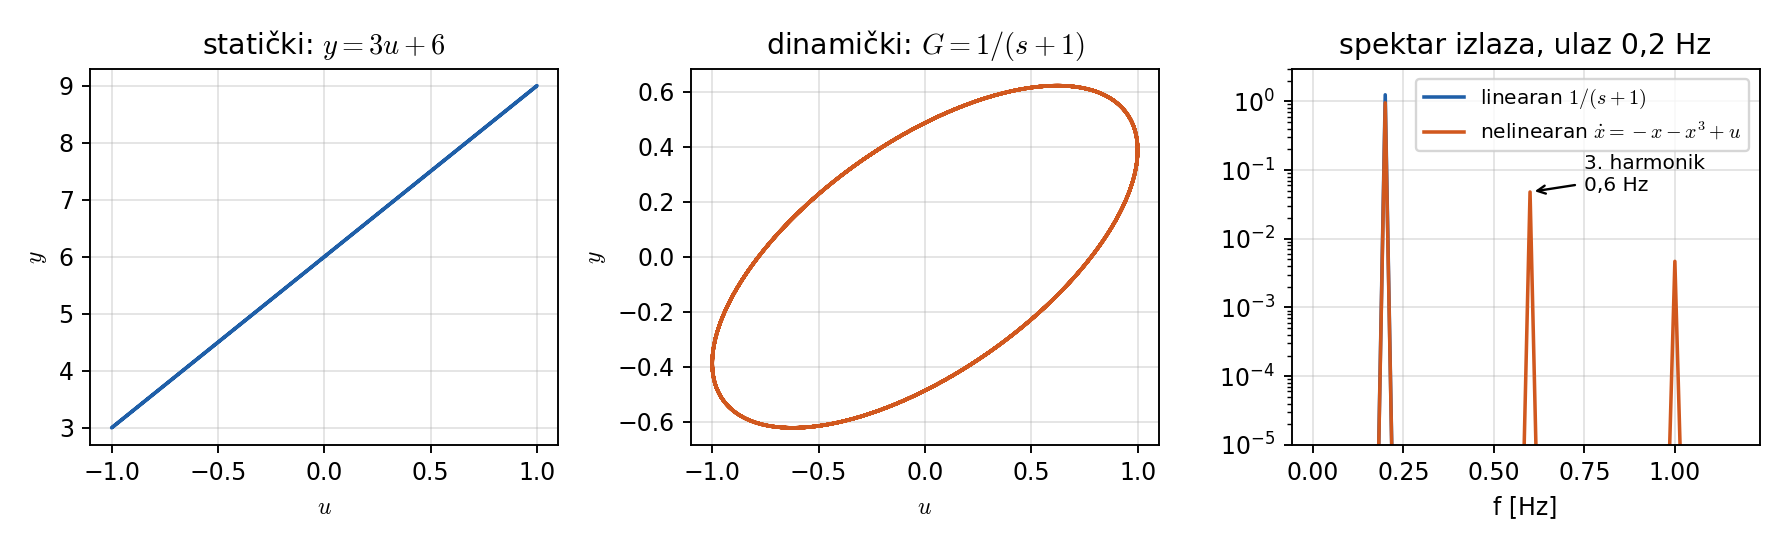
\includegraphics[width=0.95\linewidth,height=\textheight,keepaspectratio,alt={Levo: statički sistem y = 3u + 6 daje jednoznačnu krivu y(u). U sredini: dinamički sistem 1/(s+1) daje petlju, jer isti ulaz na usponu i na padu daje različit izlaz. Desno: spektar izlaza pri ulazu 0,2 Hz; linearan sistem ima samo 0,2 Hz, a nelinearan i 3. harmonik na 0,6 Hz}]{figures/modelovanje_staticki_dinamicki.png}
\caption{Levo: statički sistem y = 3u + 6 daje jednoznačnu krivu y(u). U sredini: dinamički sistem 1/(s+1) daje petlju, jer isti ulaz na usponu i na padu daje različit izlaz. Desno: spektar izlaza pri ulazu 0,2 Hz; linearan sistem ima samo 0,2 Hz, a nelinearan i 3. harmonik na 0,6 Hz}
\end{figure}

Drugi jednostavan test je odskočni ulaz: statički sistem skoči u istom trenutku, a dinamički ima prelazni proces. Tako je urađeno u tvom \texttt{zad1\_\allowbreak{}staticki\_\allowbreak{}dinamicki.m} (odziv na \(h(t-2)\) za \(y = 3u+6\) i za sistem trećeg reda).

\subsection{Linearnost}

\textbf{Definicija.} Sistem \(\mathcal M\) je linearan ako važi \textbf{superpozicija}, tj. i aditivnost i homogenost:

\[\mathcal M\{\alpha u_1 + \beta u_2\} = \alpha\,\mathcal M\{u_1\} + \beta\,\mathcal M\{u_2\}\]

Zašto dva testa: ako smeš da eksperimentišeš na postrojenju, radi se superpozicija (test a); ako imaš samo već snimljene podatke \(u\), \(y\), ostaje frekventni test (test b) \izvor{P01 snimak, 54.--56. min}.

\textbf{Test a) superpozicijom.} Simuliraju se tri odziva: \(y_1 = \mathcal M\{u_1\}\), \(y_2 = \mathcal M\{u_2\}\) i \(y_{12} = \mathcal M\{u_1 + u_2\}\), pa se proveri da li je \(y_{12} = y_1 + y_2\).

Kako se to proveri u praksi: nacrta se razlika \(e(t) = y_{12} - (y_1 + y_2)\). Kod linearnog sistema \(e\) je na nivou numeričke greške solvera (npr. \(10^{-6}\) od amplitude izlaza), a kod nelinearnog je istog reda veličine kao sam izlaz. Za \(u_1\) i \(u_2\) uzeti dva različita signala (npr. odskok i sinus), jer se nelinearnost ne vidi uvek na jednom obliku.

Na šta paziti:

\begin{itemize}
\item \textbf{Početni uslovi moraju biti nulti.} Odziv je zbir slobodnog i prinudnog. Sa \(x_0 \ne 0\) slobodni odziv se u \(y_1 + y_2\) pojavi dva puta, a u \(y_{12}\) jednom, pa bi i linearan sistem „pao'' test.
\item \textbf{\(y = 3u + 6\) nije linearan}, iako je statički. Proverimo: \(\mathcal M\{u_1\} + \mathcal M\{u_2\} = 3u_1 + 3u_2 + 12\), a \(\mathcal M\{u_1 + u_2\} = 3(u_1 + u_2) + 6\). Razlika je 6. Takav sistem se zove \textbf{afin}. Postaje linearan tek u odstupanjima od radne tačke (\(\Delta y = 3\Delta u\)).
\item Nestabilan sistem (\(\dot x = 3x + u\)) prolazi test superpozicije. Stabilnost i linearnost su nezavisne osobine.
\end{itemize}

\textbf{Test b) frekventno.} Linearan sistem ne stvara nove frekvencije. Za ulaz \(\sin\omega t\) izlaz je u ustaljenom stanju \(A\sin(\omega t + \varphi)\), iste učestanosti, samo sa drugom amplitudom i fazom. Nelinearan sistem pravi \textbf{harmonike}. Na primer, za \(\dot x = -x - x^3 + u\) član \(x^3\) od \(\sin\omega t\) daje i \(\sin 3\omega t\), jer je

\[\sin^3\omega t = \tfrac34\sin\omega t - \tfrac14\sin 3\omega t .\]

Zato se na izlazu pojavi linija na \(3\omega\) (desni grafik na slici gore). Konstanta \(+6\) kod afinog sistema daje novu liniju na 0 Hz.

Na šta paziti:

\begin{itemize}
\item analizira se samo \textbf{ustaljeno stanje}, jer prelazni proces sadrži sopstvene modove sistema, koji izgledaju kao „nove'' frekvencije;
\item test nema smisla za nestabilan sistem (nema ustaljenog stanja);
\item ulaz treba da bude \textbf{„dovoljno bogat''} (više učestanosti ili neperiodičan signal); zaključak na osnovu jedne sinusoide može biti nepouzdan \izvor{P01 snimak, 63.--65. min}. Isti zahtev se kasnije vraća kao uslov pobude kod MNK i RLS-a;
\item \textbf{nelinearnost zavisi od amplitude}: za mali ulaz je \(x^3\) zanemarljivo i nelinearan sistem izgleda linearno. Test treba ponoviti za više amplituda;
\item u FFT prozoru treba da bude ceo broj perioda, inače linija „curi'' u susedne učestanosti (leakage) i izgleda kao nova frekvencija.
\end{itemize}

\begin{zasto}
Zašto nelinearan sistem pravi nove frekvencije? Proizvod dve sinusoide je zbir sinusoida na zbiru i razlici učestanosti (\(\sin a\sin b = \tfrac12[\cos(a-b) - \cos(a+b)]\)). Svaki stepen \(x^2, x^3, \dots\) zato „meša'' učestanosti. Linearan sistem samo množi i sabira signale konstantama, pa ne može da napravi učestanost koje nije bilo na ulazu.
\end{zasto}

Vremenska invarijantnost je treća osobina iz beleški: ako \(u(t)\) daje \(y(t)\), onda \(u(t-\tau)\) daje \(y(t-\tau)\). Svi sistemi na kursu su linearni vremenski invarijantni (LTI) dok se parametri ne promene. Upravo zbog promene parametara kasnije uvodimo adaptivno upravljanje.

\subsection{Funkcija prenosa iz Bodeovog dijagrama}

\textbf{Ideja.} Kod linearnog sistema svaka učestanost prolazi nezavisno. Zato jedan eksperiment sa \textbf{zbirom sinusoida} daje ceo Bodeov dijagram odjednom.

\textbf{Postupak.}

\begin{enumerate}
\def\labelenumi{\arabic{enumi}.}
\item Na ulaz se dovede
  \[u(t) = \sum_{i=1}^{N}\sin(\omega_i t + \phi_i),\]
  sa učestanostima \(\omega_i\) raspoređenim logaritamski (dekadu ispod najnižeg i iznad najvišeg očekivanog preloma).
\item Sačeka se da prelazni proces nestane, pa se izračuna FFT ulaza i izlaza.
\item Na svakoj učestanosti \(\omega_i\) izračuna se amplitudska karakteristika
  \[|G(j\omega_i)|_{dB} = 20\log_{10}\frac{|Y(j\omega_i)|}{|U(j\omega_i)|}.\]
\item Kroz tačke se povuku asimptote. Iz \textbf{nagiba} i \textbf{prelomnih učestanosti} se čitaju polovi i nule, a iz \textbf{nivoa na niskim učestanostima} pojačanje.
\end{enumerate}

\textbf{Pravila za čitanje.} Racionalna funkcija prenosa ima nagibe samo \(\pm n\cdot 20\) dB/dek:

\begin{longtable}[]{@{}ll@{}}
\caption{Čitanje strukture iz asimptota amplitudske karakteristike}\tabularnewline
\toprule\noalign{}
Promena nagiba na \(\omega_b\) & Značenje \\
\midrule\noalign{}
\endfirsthead
\toprule\noalign{}
Promena nagiba na \(\omega_b\) & Značenje \\
\midrule\noalign{}
\endhead
\bottomrule\noalign{}
\endlastfoot
\(-20\) dB/dek & realan pol u \(s = -\omega_b\) \\
\(+20\) dB/dek & realna nula u \(s = -\omega_b\) \\
\(-40\) dB/dek & dvostruki pol (ili konjugovano-kompleksni par) \\
nagib \(-20\) od najnižih učestanosti & integrator \(1/s\) \\
konačni nagib \(-20(n-m)\) & relativni red \(n - m\) \\
\end{longtable}

Amplitudska karakteristika ne razlikuje pol u \(-a\) od pola u \(+a\) (isti moduo). Znak se čita iz \textbf{faze}: stabilan pol spušta fazu, a nestabilan je podiže. Primer sa predavanja \izvor{P01 snimak, 76.--79. min}: \(\frac{1}{s+2}\) i \(\frac{1}{s-2}\) imaju isti moduo \(1/\sqrt{\omega^2+4}\), ali je \(\arg\frac{1}{j\omega+2} = -\operatorname{arctg}\frac{\omega}{2}\) (od \(0\) pada ka \(-90°\)), a \(\arg\frac{1}{j\omega-2} = -\pi + \operatorname{arctg}\frac{\omega}{2}\) (od \(-180°\) raste ka \(-90°\)). Ako faza nije merena, pretpostavlja se minimalno-fazni stabilan sistem.

Iracionalna funkcija prenosa (npr. sistem sa raspodeljenim parametrima) ima „frakcione'' nagibe, na primer \(-8\) dB/dek. I takav sistem je linearan, samo nije konačnog reda.

\textbf{Primer.} Izmerena karakteristika na slici ispod ima: ravno do \(\omega = 0{,}2\), pa \(-20\) dB/dek, na \(\omega = 1\) ponovo ravno, a od \(\omega = 10\) opet \(-20\) dB/dek.

\begin{figure}
\centering
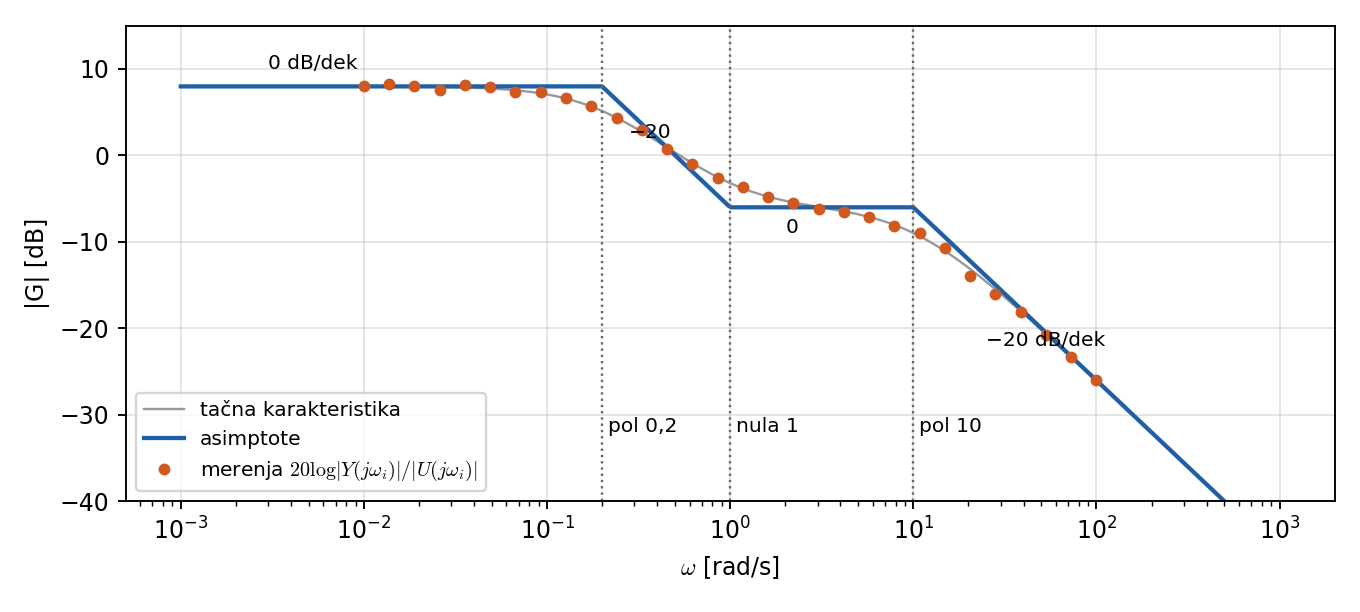
\includegraphics[width=0.85\linewidth,height=\textheight,keepaspectratio,alt={Identifikacija iz asimptota: prelomi na 0,2 (pol), 1 (nula) i 10 (pol). Nivo na niskim učestanostima je 7,96 dB, tj. statičko pojačanje 2,5}]{figures/bode_identifikacija.png}
\caption{Identifikacija iz asimptota: prelomi na 0,2 (pol), 1 (nula) i 10 (pol). Nivo na niskim učestanostima je 7,96 dB, tj. statičko pojačanje 2,5}
\end{figure}

Čitanje korak po korak:

\begin{enumerate}
\def\labelenumi{\arabic{enumi}.}
\item \(\omega = 0{,}2\): nagib \(0 \to -20\), znači pol u \(s = -0{,}2\);
\item \(\omega = 1\): nagib \(-20 \to 0\), znači nula u \(s = -1\);
\item \(\omega = 10\): nagib \(0 \to -20\), znači pol u \(s = -10\);
\item struktura je \(G(s) = K\dfrac{s+1}{(s+0{,}2)(s+10)}\);
\item nivo na niskim učestanostima je 7,96 dB, tj. \(|G(0)| = 10^{7{,}96/20} = 2{,}5\). Iz \(G(0) = K\cdot\dfrac{1}{0{,}2\cdot 10} = \dfrac{K}{2}\) sledi \(K = 5\).
\end{enumerate}

Rezultat: \(G(s) = \dfrac{5(s+1)}{(s+0{,}2)(s+10)}\). Isti rezultat daje automatsko fitovanje (\(\hat G = \frac{4{,}999(s+1)}{(s+0{,}2)(s+9{,}999)}\)).

Praktični detalji za MATLAB:

\begin{itemize}
\item učestanosti birati kao celobrojne umnoške osnovne \(2\pi/T_w\) (\(T_w\) je dužina prozora), da svaka sinusoida ima ceo broj perioda;
\item faze sinusoida birati različito (slučajno ili Schroeder-ove faze \(\phi_i = \pi i^2/N\)), inače se u \(t = 0\) sve sinusoide saberu u ogroman vrh \(N\);
\item odbaciti prvih nekoliko vremenskih konstanti (prelazni proces);
\item amplituda u dB je \(20\log_{10}\), ne prirodni logaritam;
\item najviša učestanost mora biti ispod Nikvistove, \(f_{max} < \frac{1}{2T_s}\), a praktično bar 5 puta ispod \(1/T_s\); inače se sinusoida preslika (aliasing) na nižu učestanost i pokvari Bode;
\item kako se nađe tačka na \(\omega_i\): za prozor od \(N\) odbiraka (\texttt{Y\ =\ fft(\allowbreak{}y)}, \(T_w = NT_s\)) element \texttt{Y(k+1)} odgovara učestanosti \(f = k/T_w\). Ako je \(\omega_i = 2\pi k_i/T_w\), amplituda je \texttt{abs(\allowbreak{}Y(\allowbreak{}ki+1)/\allowbreak{}U(\allowbreak{}ki+1))}, a faza \texttt{angle(\allowbreak{}Y(\allowbreak{}ki+1)/\allowbreak{}U(\allowbreak{}ki+1))}.
\end{itemize}

Provera rezultata: preko izmerenih tačaka nacrtaj \texttt{bode} dobijenog \(G(s)\). Tačke treba da leže na krivoj i u amplitudi i u fazi; ako faza odstupa sistematski, znak nekog pola ili nule je pogrešan.

\begin{ispit}
Na odbrani prvog domaćeg: statički znači bez memorije (\(y(u)\) je kriva, ne petlja). Linearnost se proverava superpozicijom uz \textbf{nulte početne uslove} i frekventno, samo u ustaljenom stanju stabilnog sistema. \(y = 3u + 6\) je statički, ali afin, pa \textbf{nije} linearan. Iz Bodeovog dijagrama: nagibi daju red, prelomi daju polove i nule, nivo na niskim učestanostima daje pojačanje, a faza daje znak.
\end{ispit}

\section{Identifikacija parametara i metod najmanjih kvadrata}

\subsection{Ideja}

Kada znamo strukturu modela (red, broj polova i nula), ostaje da odredimo brojeve u njemu. Trik je da se diferencijalna (ili diferencna) jednačina zapiše tako da bude \textbf{linearna po nepoznatim parametrima}. Tada je svako merenje jedna linearna jednačina, a sa dovoljno merenja parametri se dobijaju rešavanjem sistema linearnih jednačina. Isti oblik \(\eta = \varphi^T\theta\) kasnije koriste i RLS i gradijentni algoritam, pa je ovo osnova celog adaptivnog dela.

Identifikacija je u suštini optimizacija (traži se \(\theta\) koje minimizuje grešku modela). Mogli bi se koristiti i opšti algoritmi (PSO, genetski), ali oni ne garantuju globalni optimum; kada parametri ulaze \textbf{linearno}, namenski MNK daje tačan optimum u jednom koraku \izvor{P02 snimak, 0.--7. min}. Oznake: kapica je procena (\(\hat\theta\)), tilda je greška, \textbf{stvarno minus procenjeno} (\(\tilde\eta = \eta - \hat\eta\)).

\subsection{\texorpdfstring{Linearna parametrizacija \(\eta = \varphi^T\theta\)}{Linearna parametrizacija \textbackslash eta = \textbackslash varphi\^{}T\textbackslash theta}}

\textbf{Postavka.}

\[\eta = \varphi_1\theta_1 + \varphi_2\theta_2 + \dots + \varphi_n\theta_n = \varphi^T\theta\]

\begin{itemize}
\item \(\eta\) je merljiva veličina, po dogovoru \textbf{najviši izvod} izlaza (ili najnoviji odbirak);
\item \(\varphi = [\varphi_1 \dots \varphi_n]^T\) je \textbf{regresioni vektor}: merljive veličine koje se menjaju u vremenu;
\item \(\theta = [\theta_1 \dots \theta_n]^T\) su nepoznati parametri, konstantni u vremenu.
\end{itemize}

\textbf{Kontinualni sistem, korak po korak.} Neka je

\[G(s) = \frac{Y(s)}{U(s)} = \frac{b_1 s + b_0}{s^2 + a_1 s + a_0}.\]

\begin{enumerate}
\def\labelenumi{\arabic{enumi}.}
\item Pomnožimo unakrsno: \(s^2Y + a_1 sY + a_0 Y = b_1 sU + b_0 U\).
\item Inverzna Laplasova transformacija (nulti početni uslovi): \(\ddot y + a_1\dot y + a_0 y = b_1\dot u + b_0 u\).
\item Najviši izvod ostavimo levo:
  \[\ddot y = -a_1\dot y - a_0 y + b_1\dot u + b_0 u .\]
\item Očitamo:
  \[\eta = \ddot y,\qquad \varphi = [-\dot y\;\; -y\;\; \dot u\;\; u]^T,\qquad \theta = [a_1\;\; a_0\;\; b_1\;\; b_0]^T .\]
\end{enumerate}

Minus ispred \(\dot y\) i \(y\) stoji u \(\varphi\) da bi u \(\theta\) bili koeficijenti imenioca sa istim znakom kao u \(G(s)\). (U nekim zapisima znak stoji jednom uz \(\theta\), a jednom uz \(\varphi\); oba izbora su ispravna ako se dosledno koriste.)

\textbf{Diskretni sistem.} Neka je \(G(z) = \dfrac{b_1 z + b_0}{z^2 + a_1 z + a_0}\). Brojilac i imenilac podelimo sa \(z^2\) i koristimo \(z^{-1}y(k) = y(k-1)\):

\[y(k) = -a_1 y(k-1) - a_0 y(k-2) + b_1 u(k-1) + b_0 u(k-2),\]

\[\eta = y(k),\qquad \varphi = [-y(k-1)\;\; -y(k-2)\;\; u(k-1)\;\; u(k-2)]^T .\]

U diskretnom slučaju nema izvoda, nego samo prošlih odbiraka, a njih već imamo u memoriji. Zato diskretna identifikacija ne mora da filtrira signale. Ako se ipak filtrira zbog šuma, najprostiji niskopropusni filter je \(\frac{1-\alpha}{z-\alpha}\), \(0 < \alpha < 1\) (jedinično statičko pojačanje), isti za \(u\) i \(y\) \izvor{P02 snimak, 104.--107. min}.

\textbf{Kako se \(\Phi\) složi u MATLAB-u.} Za kolone \texttt{y}, \texttt{u} sa \(N\) odbiraka (perioda \(T_s\)) svaka vrsta je jedno \(k\). Prva upotrebljiva vrsta je \(k = 3\), jer tek tada postoji \(y(k-2)\):

\begin{verbatim}
eta = y(3:N);
Phi = [-y(2:N-1), -y(1:N-2), u(2:N-1), u(1:N-2)];   % k-1 i k-2
theta = Phi \ eta;
\end{verbatim}

Svi vektori moraju imati \(N-2\) vrsta i biti pomereni za isti \(k\). U Simulinku isto daju blokovi \emph{Unit Delay} (\(z^{-1}\)): \(y \to z^{-1} \to y(k-1) \to z^{-1} \to y(k-2)\).

Ako se ovako identifikuje \textbf{kontinualni} proces iz odbiraka, dobijeni \(\theta\) su koeficijenti od \texttt{c2d(\allowbreak{}G,\allowbreak{}\ Ts)} (ZOH), a ne od \(G(s)\). Nazad se ide sa \texttt{d2c(\allowbreak{}tf(\allowbreak{}{[}b1\ b0{]},\allowbreak{}\ {[}1\ a1\ a0{]},\allowbreak{}\ Ts))}.

\subsection{Filtriranje: zašto i kako}

\textbf{Problem.} U kontinualnom slučaju \(\eta = \ddot y\) i \(\varphi\) sadrže izvode, a izvodi se ne mere. Numeričko diferenciranje pojačava šum, a \(sY(s)\) nije kauzalna funkcija prenosa, pa ne može biti blok u Simulinku.

\textbf{Rešenje.} Celu jednačinu podelimo istim stabilnim polinomom \((T_f s + 1)^n\), gde je \(n\) red sistema:

\[\frac{s^2}{(T_fs+1)^2}Y = -a_1\frac{s}{(T_fs+1)^2}Y - a_0\frac{1}{(T_fs+1)^2}Y + b_1\frac{s}{(T_fs+1)^2}U + b_0\frac{1}{(T_fs+1)^2}U .\]

Svaki razlomak je sada kauzalan, pa je svaki član izlaz nekog filtra oblika

\[F_m(s) = \frac{s^m}{(T_f s + 1)^n},\qquad m = 0, 1, \dots, n,\]

gde je \(m\) red izvoda te promenljive. Dobija se ista jednačina, samo sa filtriranim signalima:

\[\ddot y_f = -a_1\dot y_f - a_0 y_f + b_1\dot u_f + b_0 u_f .\]

\begin{figure}
\centering
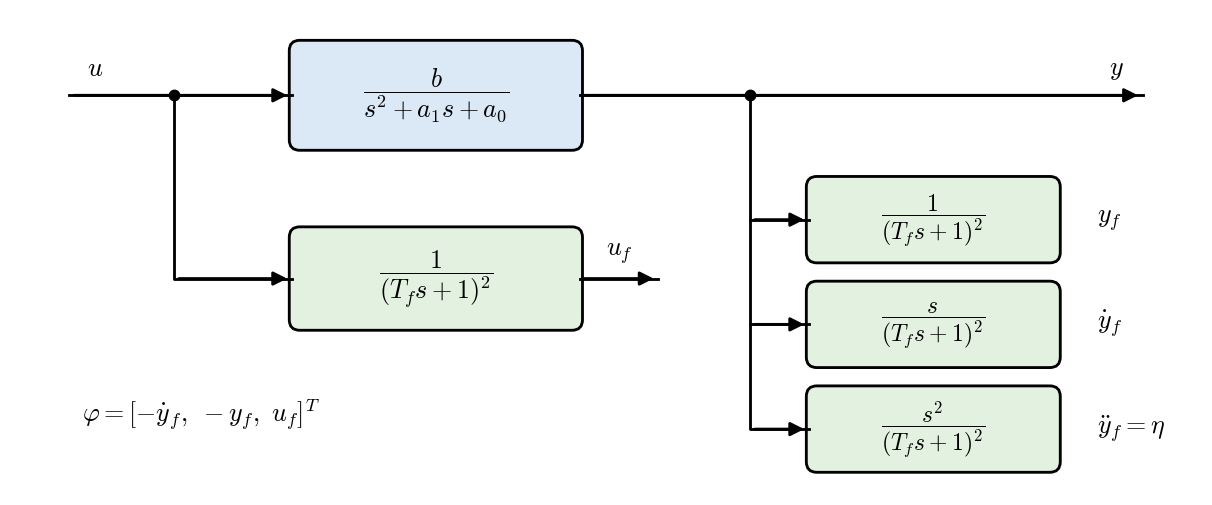
\includegraphics[width=0.85\linewidth,height=\textheight,keepaspectratio,alt={Filtri za identifikaciju procesa drugog reda: isti imenilac (Tf·s + 1)² za sve signale, a brojilac s\^{}m daje filtrirani m-ti izvod. Ulaz mora da prođe kroz isti filter kao izlaz}]{figures/blok_filtri.png}
\caption{Filtri za identifikaciju procesa drugog reda: isti imenilac (Tf·s + 1)² za sve signale, a brojilac s\^{}m daje filtrirani m-ti izvod. Ulaz mora da prođe kroz isti filter kao izlaz}
\end{figure}

\begin{kljucna}
Isti filter na obe strane jednačine \textbf{ne menja} \(\theta\), jer je filter linearan i vremenski nepromenljiv. Zato i \(u\) mora proći kroz filter sa istim imeniocem. Stepen imenioca \(n\) mora biti bar jednak najvišem izvodu, da bi \(s^n/(T_fs+1)^n\) bio kauzalan.
\end{kljucna}

U Simulinku je svaki filter jedan blok \emph{Transfer Fcn}, npr. za \(n = 2\): brojilac \texttt{{[}1\ 0\ 0{]}}, \texttt{{[}1\ 0{]}} ili \texttt{1}, imenilac \texttt{conv(\allowbreak{}{[}Tf\ 1{]},\allowbreak{}{[}Tf\ 1{]})}; izlazi idu u \emph{To Workspace}. Bez Simulinka isto radi \texttt{lsim(\allowbreak{}tf(\allowbreak{}{[}1\ 0{]},\allowbreak{}{[}Tf\ 1{]}),\allowbreak{}\ y,\allowbreak{}\ t)}. Filtri kreću iz nultih početnih uslova, pa je potrebno i da proces kreće iz nule, ili da se odbaci prvih nekoliko \(T_f\).

Izbor \(T_f\): filter treba da bude brži od procesa (npr. \(T_f\) nekoliko puta manje od najmanje vremenske konstante procesa), ali ne previše. \(\ddot y_f\) na visokim učestanostima ima pojačanje do \(1/T_f^2\), pa malo \(T_f\) jako pojačava merni šum. Bez šuma, u simulaciji, radi i sporiji filter (u tvom \texttt{kontinualan\_\allowbreak{}sistem.m} je \(T_f = 1\) za proces sa polom u \(-2\)).

Uslov sa predavanja: filter \textbf{ne sme da odseče korisne učestanosti ulaza}, tj. \(1/T_f\) treba da bude iznad najviše učestanosti u \(u\) \izvor{P02 snimak, 79.--81. min}. Kompromis je pokazan uživo \izvor{P02 snimak, 91.--104. min}: ulaz je zbir sinusoida 0,1 do 5 rad/s, proces drugog reda sa 4 parametra; bez šuma \(T_f = 0{,}05\) daje tačne parametre, a sa šumom \(\pm 0{,}05\) na izlazu procene primetno odstupaju od tačnih (dobijeno je 2,19; 5,54; 0,94; 3,38). Sa \(T_f = 0{,}5\) (sporiji filter, jače guši šum, a još propušta ulazne učestanosti) procene su tačne na drugu decimalu.

Alternativa filtrima je blok \emph{Derivative} u Simulinku, ali on pojačava šum, pa se na kursu koriste filtri \izvor{P02 snimak, 71.--78. min}.

\subsection{\texorpdfstring{Osnovni algoritam: tačno \(n\) merenja}{Osnovni algoritam: tačno n merenja}}

Za \(n\) nepoznatih uzmemo \(n\) merenja u trenucima \(1, \dots, n\):

\[
\begin{aligned}
\eta^{(1)} &= \varphi_1^{(1)}\theta_1 + \dots + \varphi_n^{(1)}\theta_n\\
&\;\;\vdots\\
\eta^{(n)} &= \varphi_1^{(n)}\theta_1 + \dots + \varphi_n^{(n)}\theta_n
\end{aligned}
\qquad\Longrightarrow\qquad
\boldsymbol\eta_{n\times 1} = \Phi_{n\times n}\,\theta,\qquad \theta = \Phi^{-1}\boldsymbol\eta .
\]

Svaka vrsta matrice \(\Phi\) je \(\varphi^T\) u jednom trenutku. Inverzija postoji samo ako je \(\Phi\) \textbf{punog ranga} (kolone linearno nezavisne).

\textbf{Kada \(\Phi\) nije punog ranga.} Primer: \(u = \text{const}\). Posle smirenja je \(u(k-1) = u(k-2)\) i \(y(k-1) = y(k-2)\), pa su po dve kolone jednake i rang pada. U kontinualnom slučaju kolona \(\dot u\) postaje nula. Za diskretni primer se dobija rang 1 od 4.

\begin{kljucna}
Ulaz mora \textbf{dovoljno da pobudi} sistem (persistent excitation). \textbf{Pravilo kursa:} za \(n\) nepoznatih parametara ulaz mora imati \textbf{bar \(n\) različitih učestanosti}, „jednako, a bolje i više od broja parametara''; za 4 parametra zbir bar četiri sinusoide \izvor{P02 snimak, 29.--37. min}. U praksi: zbir sinusoida, pseudoslučajni \(\pm 1\) signal ili šum.
\end{kljucna}

\textbf{Teorijski minimum} (matematička činjenica, ne pravilo sa predavanja): jedna sinusoida daje dve nezavisne kolone (amplituda i faza), pa je strogo potrebno \(\lceil n/2\rceil\) različitih učestanosti, a ako \(\theta\) sadrži i konstantni član (offset), još i konstanta na ulazu. Sa samo \(\lceil n/2\rceil\) sinusoida je \(\Phi\) na granici ranga i loše uslovljena čim ima šuma, pa se na domaćem i na odbrani drži pravila kursa (\(\ge n\)).

\subsection{Metod najmanjih kvadrata (MNK)}

\textbf{Postavka.} U praksi merenja imaju šum, pa se uzima \(N \gg n\) merenja. Tada je \(\Phi\) dimenzija \(N\times n\), nije kvadratna i nema inverz. Traži se \(\hat\theta\) koje \textbf{najbolje} objašnjava sva merenja:

\[\hat\eta^{(i)} = \varphi^{(i)T}\hat\theta,\qquad \tilde\eta^{(i)} = \eta^{(i)} - \hat\eta^{(i)},\qquad J = \frac12\sum_{i=1}^{N}\big(\tilde\eta^{(i)}\big)^2 \to \min .\]

\textbf{Izvođenje.}

\begin{enumerate}
\def\labelenumi{\arabic{enumi}.}
\item Uslov minimuma je da je izvod po svakom parametru nula, \(j = 1,\dots,n\):
  \[\frac{\partial J}{\partial\hat\theta_j} = \frac12\sum_{i=1}^N 2\,\tilde\eta^{(i)}\,\frac{\partial\tilde\eta^{(i)}}{\partial\hat\theta_j} = \sum_{i=1}^N \tilde\eta^{(i)}\big(-\varphi_j^{(i)}\big) = 0 .\]
\item Zamenimo \(\tilde\eta^{(i)} = \eta^{(i)} - \sum_k\varphi_k^{(i)}\hat\theta_k\) i prebacimo članove sa \(\hat\theta\) na desnu stranu:
  \[\sum_{i=1}^N\varphi_j^{(i)}\eta^{(i)} = \sum_{k=1}^n\Big(\sum_{i=1}^N\varphi_j^{(i)}\varphi_k^{(i)}\Big)\hat\theta_k,\qquad j = 1,\dots,n .\]
\item Leva strana je \(j\)-ti element vektora \(\Phi^T\boldsymbol\eta\), a zagrada na desnoj strani je element \((j,k)\) matrice \(\Phi^T\Phi\). Svih \(n\) jednačina zajedno su \textbf{normalne jednačine}:
  \[\Phi^T\Phi\,\hat\theta = \Phi^T\boldsymbol\eta .\]
\item \(\Phi^T\Phi\) je kvadratna \(n\times n\). Ako je \(\Phi\) punog ranga po kolonama, ona je invertibilna:
\end{enumerate}

\[\hat\theta = (\Phi^T\Phi)^{-1}\Phi^T\boldsymbol\eta\]

Matrica \((\Phi^T\Phi)^{-1}\Phi^T\) je \textbf{pseudoinverzija} matrice \(\Phi\). U MATLAB-u: \texttt{theta\ =\ Phi\textbackslash{}eta} ili \texttt{pinv(\allowbreak{}Phi)*eta}. Operator \texttt{\textbackslash{}} koristi QR dekompoziciju i numerički je bolji od \texttt{inv(\allowbreak{}Phi\textquotesingle{}*Phi)*Phi\textquotesingle{}*eta}, jer ne kvadrira uslovljenost matrice.

\begin{zasto}
Zašto više merenja pomaže? Kriterijum \(J\) sabira kvadrate grešaka, pa se nezavisni šumovi u različitim merenjima delimično poništavaju (usrednjavaju). Sa tačno \(n\) merenja \(\Phi^{-1}\) prenosi šum direktno u \(\theta\). Sa šumom \(\sigma = 0{,}05\) i 4 merenja dobija se \([0{,}45;\ 0{,}63;\ 0{,}07;\ 0{,}15]\) umesto \([0{,}2;\ 0{,}3;\ 0{,}1;\ 0{,}2]\), a sa \(N \approx 5000\) merenja \([0{,}19;\ 0{,}28;\ 0{,}10;\ 0{,}20]\).
\end{zasto}

\textbf{Pristrasnost (bias).} Ako je šum u izlazu, a prošli izlazi su u \(\varphi\), onda je regresor korelisan sa greškom. Tada greška procene ne pada na nulu ni za veliko \(N\), nego se zaustavi na nekoj vrednosti (slika). To je poznato ograničenje običnog MNK. Za kurs je dovoljno znati \textbf{zašto} se dešava. (Druga vrsta pristrasnosti, od konstantnog poremećaja na ulazu, i njen lek sa predavanja, propusnik opsega na signalima za identifikaciju, opisani su u poglavlju o projektu.)

\begin{figure}
\centering
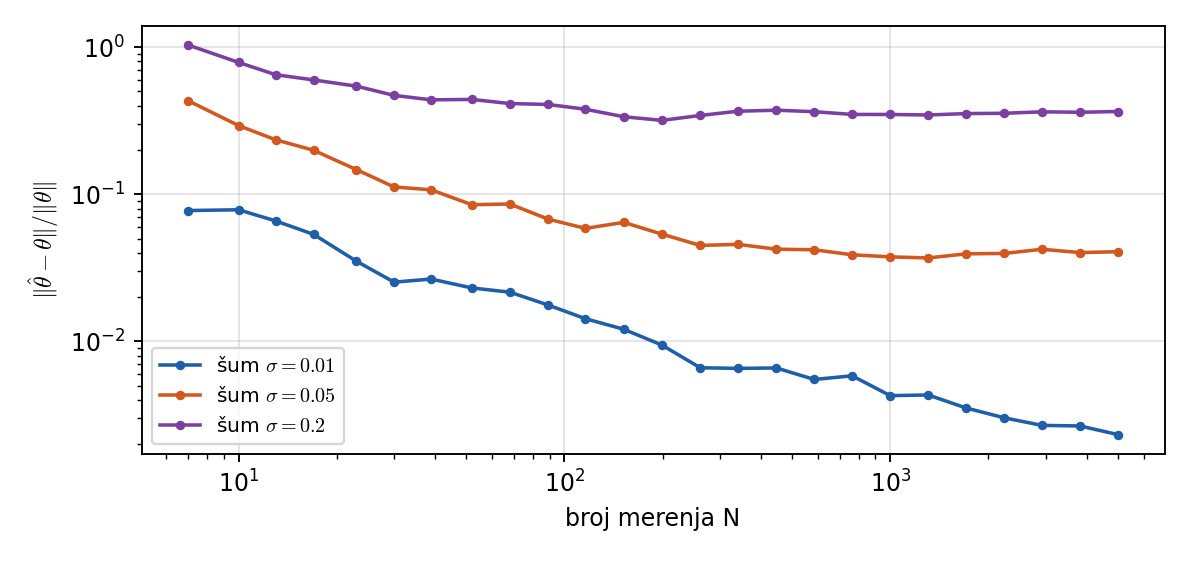
\includegraphics[width=0.75\linewidth,height=\textheight,keepaspectratio,alt={Relativna greška MNK procene u zavisnosti od broja merenja N (diskretni sistem iz domaćeg, ulaz ±1). Za mali šum greška pada sa N. Za veći šum (σ = 0,2) opadanje prestaje, jer je šum i u regresoru φ}]{figures/mnk_greska_N.png}
\caption{Relativna greška MNK procene u zavisnosti od broja merenja N (diskretni sistem iz domaćeg, ulaz ±1). Za mali šum greška pada sa N. Za veći šum (σ = 0,2) opadanje prestaje, jer je šum i u regresoru φ}
\end{figure}

\subsection{Primer: proces prvog reda (pojednostavljenje domaćeg 2)}

Domaći 2 diktiran na predavanju je proces \textbf{drugog reda sa 4 parametra}, \(G(s) = \frac{b_1s + b_0}{s^2 + a_1s + a_0}\) (parametrizacija iz odeljka gore), sa filtrima \(s^m/(T_fs+1)^2\), bar 4 sinusoide, bez i sa šumom, pa isto diskretno \izvor{P02 snimak, 67.--81. i 104.--106. min}; tekst je u mapi domaćih. Tvoje rešenje radi pojednostavljenu varijantu prvog reda, pa je ona ovde primer; za predaju uradi zadatak drugog reda.

Proces \(G(s) = \dfrac{a}{s + b}\), sa \(a = 1\), \(b = 2\).

\begin{enumerate}
\def\labelenumi{\arabic{enumi}.}
\item \(sY + bY = aU\), pa je \(\dot y = -b\,y + a\,u\).
\item Filter prvog reda (\(n = 1\)): \(\dot y_f = \dfrac{s}{T_fs+1}y\), \(y_f = \dfrac{1}{T_fs+1}y\), \(u_f = \dfrac{1}{T_fs+1}u\).
\item \(\eta = \dot y_f\), \(\varphi = [-y_f\;\; u_f]^T\), \(\theta = [b\;\; a]^T\).
\item Ulaz: zbir sinusoida. Za 2 parametra je teorijski dovoljna jedna sinusoida, a po pravilu kursa uzeti bar dve.
\item \texttt{Theta\ =\ {[}-y\_\allowbreak{}f,\allowbreak{}\ u\_\allowbreak{}f{]}\ \textbackslash{}\ y\_\allowbreak{}p}, gde je \texttt{y\_p} \(= \dot y_f\), pa \texttt{b\ =\ Theta(\allowbreak{}1)}, \texttt{a\ =\ Theta(\allowbreak{}2)}.
\end{enumerate}

U tvom skriptu \texttt{kontinualan\_\allowbreak{}sistem.m} je \(\varphi = [-y_f,\ u_f]\) i posle toga \texttt{b\_\allowbreak{}hat\ =\ -Theta(\allowbreak{}1)}. Sa minusom već u \(\varphi\), \(\theta_1\) je direktno \(b\), pa dodatni minus daje \(\hat b = -2\) umesto \(2\). Proveri znak kad budeš radio domaći (vidi i spisak otvorenih pitanja).

\textbf{Diskretni primer (domaći).} \(G(z) = \dfrac{0{,}1z + 0{,}2}{z^2 + 0{,}2z + 0{,}3}\) daje \(y(k) = -0{,}2y(k-1) - 0{,}3y(k-2) + 0{,}1u(k-1) + 0{,}2u(k-2)\), pa je \(\theta = [0{,}2;\ 0{,}3;\ 0{,}1;\ 0{,}2]\). Posle identifikacije model treba \textbf{validirati}: simulirati ga na novom ulazu, koji nije korišćen za identifikaciju, i uporediti sa merenjem.

Šta je „dobro'': bez šuma se \(\hat\theta\) poklapa sa tačnim na 3 do 4 decimale, a greška \(\boldsymbol\eta - \Phi\hat\theta\) je na nivou numeričke greške. Ako nije, najčešći uzroci su pomereni indeksi (\(k-1\) naspram \(k\)), pogrešan izvod za \(\eta\) (npr. \(\dot y_f\) umesto \(\ddot y_f\), greška viđena i uživo na času \izvor{P02 snimak, 91.--104. min}), pogrešan znak u \(\varphi\), \(u\) bez istog filtra kao \(y\), ili siromašan ulaz (proveri \texttt{rank(Phi)} i \texttt{cond(Phi)}).

\begin{ispit}
Znati izvesti \(\hat\theta = (\Phi^T\Phi)^{-1}\Phi^T\eta\) iz \(\partial J/\partial\hat\theta = 0\) i objasniti: \(\eta\) je najviši izvod ili najnoviji odbirak, \(\varphi\) je merljivo, \(\theta\) je nepoznato. Kontinualno se filtrira sa \(s^m/(T_fs+1)^n\), i to \textbf{isti imenilac za \(u\) i \(y\)}. \(\Phi\) mora biti punog ranga, pa ulaz mora biti bogat. Na odbrani navesti \textbf{pravilo sa predavanja: bar \(n\) učestanosti za \(n\) parametara}, a tek zatim napomenu da je teorijski minimum \(\lceil n/2\rceil\). Česta zamka: konstantan ulaz ili samo jedna sinusoida za 3 ili više parametara.
\end{ispit}

\section{Regulator po stanjima, observer i regulator po izlazima}

\subsection{Ideja}

Indirektno adaptivno upravljanje u projektu koristi \textbf{regulator po stanjima sa observerom}. Kada se parametri procesa promene, ponovo se računaju pojačanja \(K\), \(L\) i \(k_r\). Zato ovde treba potpuno razumeti kako se ta pojačanja dobijaju iz matrica \(A\), \(B\), \(C\). Tri koraka su:

\begin{enumerate}
\def\labelenumi{\arabic{enumi}.}
\item regulator po stanjima \(u = -Kx + k_r r\) postavlja polove zatvorene sprege gde želimo;
\item observer procenjuje stanja koja ne merimo;
\item regulator po izlazima je spoj ta dva, a princip separacije kaže da se \(K\) i \(L\) projektuju nezavisno.
\end{enumerate}

\subsection{Motivacija: servo sistem i P/PD regulator}

Motor sa upravljanjem pozicijom ima model:

\[\dot x_1 = x_2,\qquad \dot x_2 = -\frac{1}{T_p}x_2 + \frac{K}{T_p}u,\qquad y = x_1,\qquad G(s) = \frac{K}{s(T_ps+1)} .\]

Ovo je \textbf{primer koji se vuče do kraja semestra} \izvor{P03 snimak, 0.--5. min}: isti motor se koristi za regulator po stanjima, observer, estimator poremećaja, RST i projekat, pa ga treba znati napamet. Redosled zahteva je: prvo stabilnost, pa nulta greška u ustaljenom stanju. Motor već ima integrator (astatizam), pa za konstantnu referencu bez poremećaja već P regulator daje nultu grešku; nepotreban dodatni integrator samo smanjuje pretek stabilnosti \izvor{P03 snimak, 8.--10. min}.

\textbf{P regulator} \(u = K_p(r - y)\): karakteristični polinom zatvorene sprege je

\[f(s) = s(T_ps+1) + KK_p = T_p\Big(s^2 + \frac{1}{T_p}s + \frac{KK_p}{T_p}\Big).\]

Sistem je drugog reda, a imamo jedan parametar. Zbir polova je uvek \(-1/T_p\), pa polove ne možemo postaviti proizvoljno. (Česta greška: propustiti \(1/T_p\) uz \(s\).)

\textbf{PD regulator} \(u = K_pe + K_d\dot e\): \(f(s) = T_p\big(s^2 + \frac{1 + KK_d}{T_p}s + \frac{KK_p}{T_p}\big)\). Sada imamo dva parametra za dva koeficijenta, pa je raspored polova proizvoljan. Ali idealni PD nije realizabilan (stepen brojioca veći od imenioca) i diferencira šum. Realni PD je \(K_p\frac{1 + T_ds}{T_fs+1}\), sa preporukom \(T_d/T_f = 4\) do \(20\) \izvor{P03 snimak, 39.--50. min}. On podiže red na 3, a \(T_f\) nije slobodan parametar (određuje ga koliko šuma treba filtrirati), pa ostaju 2 parametra za 3 pola.

\begin{zasto}
Zašto ne izabrati \(T_d = T_p\), pa „skratiti'' pol procesa nulom regulatora? Na papiru se pol skrati, ali fizički ostaje: na njega se više ne može uticati (grana GMK se zatvara sama u sebe), pa lako postane dominantan. Ako je taj pol nestabilan (npr. \(\frac{1}{s(s-3)}\)), skraćivanje je potpuno pogrešno: nestabilan mod ostaje u sistemu, a \(T_d\) bi bila i negativna \izvor{P03 snimak, 29.--35. min}.
\end{zasto}

Zaključak: \textbf{za proces reda \(n\) treba \(n\) podesivih parametara}. Regulator po stanjima to daje direktno: po jedno pojačanje za svako stanje. PD je u stvari regulator po stanjima za \(x_1 = e\), \(x_2 = \dot e\).

\subsection{Regulator po stanjima}

\textbf{Postavka.}

\[\dot x = Ax + Bu,\qquad y = Cx,\qquad u = -Kx + k_r r = -k_1x_1 - \dots - k_nx_n + k_r r .\]

\textbf{Izvođenje zatvorene sprege.} Zamenimo \(u\) u jednačinu stanja:

\[\dot x = Ax + B(-Kx + k_r r) = (A - BK)x + Bk_r r .\]

Polovi zatvorene sprege su koreni karakterističnog polinoma

\[f_{cl}(s) = \det\big(sI - (A - BK)\big).\]

Izjednačimo \(f_{cl}(s)\) sa željenim polinomom (npr. \((s+p)^n\)) i dobijemo \(n\) jednačina za \(k_1,\dots,k_n\). MATLAB to radi Akermanovom formulom: \texttt{K\ =\ acker(\allowbreak{}A,\allowbreak{}\ B,\allowbreak{}\ polovi)} (ili \texttt{place}, koji traži različite polove).

\textbf{Primer (motor iz vežbi).} \(T_p = 0{,}5\), \(K = 2\), pa je \(A = \begin{bmatrix}0 & 1\\ 0 & -2\end{bmatrix}\), \(B = \begin{bmatrix}0\\ 4\end{bmatrix}\). Željeni polovi su \(-1, -1\).

\begin{enumerate}
\def\labelenumi{\arabic{enumi}.}
\item \(BK = \begin{bmatrix}0 & 0\\ 4k_1 & 4k_2\end{bmatrix}\), pa je \(A - BK = \begin{bmatrix}0 & 1\\ -4k_1 & -2 - 4k_2\end{bmatrix}\).
\item \(\det\begin{bmatrix}s & -1\\ 4k_1 & s + 2 + 4k_2\end{bmatrix} = s^2 + (2 + 4k_2)s + 4k_1\).
\item Željeno: \((s+1)^2 = s^2 + 2s + 1\).
\item Izjednačavanje: \(2 + 4k_2 = 2 \Rightarrow k_2 = 0\) i \(4k_1 = 1 \Rightarrow k_1 = 0{,}25\).
\end{enumerate}

Za opšti motor važi \(p_1 + p_2 = \frac{1}{T_p}(1 + Kk_2)\) i \(p_1p_2 = \frac{K}{T_p}k_1\).

\textbf{Kako izabrati polove regulatora.} Polaziš od polova procesa i od zahteva za brzinu:

\begin{itemize}
\item dvostruki pol u \(-p\) daje odziv bez preskoka, koji se smiri (u 2 \%) za oko \(5{,}8/p\) sekundi, jer je odskočni odziv \(1 - e^{-pt}(1 + pt)\);
\item brži polovi traže veća pojačanja. Za motor je \(k_1 = p^2T_p/K\), a u trenutku skoka reference (uz \(x = 0\)) je \(u = k_rr = k_1r\). Dvostruko brži polovi znače četiri puta veći skok upravljanja: za \(p = 1\) je \(k_1 = 0{,}25\), a za \(p = 5\) već \(6{,}25\);
\item razuman početak: polovi istog reda kao najbrži pol procesa, do oko 3 puta brži (u primeru proces ima pol u \(-2\), a regulator \(-1\) do \(-3\)). Ovo je standardna praksa, nije rečeno na predavanju. Pogledaj \(u(t)\): ako je nerealno veliko, uspori polove.
\end{itemize}

\subsection{Upravljivost (kontrolabilnost)}

\textbf{Primer gde ne radi}: \(\dot x_1 = x_1 + u\), \(\dot x_2 = x_2\), polovi treba da budu u \(-1\).

\[A - BK = \begin{bmatrix}1 - k_1 & -k_2\\ 0 & 1\end{bmatrix},\qquad \det(sI - A + BK) = (s - 1 + k_1)(s - 1).\]

\(k_2\) uopšte ne figuriše, a pol \(s = 1\) ostaje gde je, šta god izabrali. Razlog se vidi iz modela: na \(x_2\) ne utiče ni \(u\) ni \(x_1\). Ovakva „vizuelna'' provera iz jednačina (prati se lanac \(u \to x_i \to x_j\)) je dobar prvi korak na odbrani, pre računanja ranga \izvor{P04 snimak, 23.--29. min}.

\textbf{Definicija.} Sistem je upravljiv ako ulaz utiče na sva stanja (direktno ili preko drugih stanja) tako da im se vrednosti mogu nezavisno podešavati. Test:

\[W_c = [B\;\; AB\;\; A^2B\;\; \dots\;\; A^{n-1}B],\qquad \text{sistem je upravljiv} \iff \operatorname{rang}W_c = n .\]

U MATLAB-u: \texttt{rank(\allowbreak{}ctrb(\allowbreak{}A,\allowbreak{}B))}. Za primer: \(W_c = \begin{bmatrix}1 & 1\\ 0 & 0\end{bmatrix}\), rang 1 \textless{} 2. Ako bi bilo \(\dot x_2 = x_1\), \(x_2\) bi se upravljao posredno preko \(x_1\), i rang bi bio 2.

\begin{kljucna}
Polovi se mogu proizvoljno postaviti \textbf{ako i samo ako} je par \((A, B)\) upravljiv. Posledica u adaptivnoj šemi (\(\hat b \to 0\)): vidi Uvod u adaptivno upravljanje.
\end{kljucna}

\subsection{\texorpdfstring{Pojačanje reference \(k_r\)}{Pojačanje reference k\_r}}

Bez \(k_r r\) regulator samo vraća stanje u nulu. To je dovoljno kod linearizovanog modela oko radne tačke. Kod servo sistema izlaz treba da prati referencu, pa se \(k_r\) bira tako da \textbf{statičko pojačanje} od \(r\) do \(y\) bude 1.

\textbf{Opšte izvođenje.} U ustaljenom stanju je \(\dot x = 0\):

\[0 = (A - BK)x_{ss} + Bk_r r \;\Rightarrow\; x_{ss} = -(A - BK)^{-1}Bk_r r \;\Rightarrow\; y_{ss} = -C(A - BK)^{-1}B\,k_r r .\]

Iz \(y_{ss} = r\) sledi

\[k_r = \frac{1}{C(BK - A)^{-1}B} = \frac{1}{G_{cl}(0)},\qquad G_{cl}(s) = C(sI - A + BK)^{-1}B .\]

U MATLAB-u (kao u tvojim skriptama): \texttt{kr\ =\ 1/\allowbreak{}dcgain(\allowbreak{}ss(\allowbreak{}A-B*K,\allowbreak{}\ B,\allowbreak{}\ C,\allowbreak{}\ 0))}.

\textbf{Za motor} je \(G_{cl}(s) = \dfrac{\frac{K}{T_p}}{s^2 + \frac{1}{T_p}(1+Kk_2)s + \frac{K}{T_p}k_1}\), pa je \(G_{cl}(0) = 1/k_1\) i \(k_r = k_1\). U primeru iznad \(k_r = 0{,}25\).

\textbf{Diskretno} (\(x(k+1) = A_dx(k) + B_du(k)\)): ustaljeno stanje je \(x_{ss} = (A_d - B_dK)x_{ss} + B_dk_r r\), pa je \(k_r = 1/\big(C(I - A_d + B_dK)^{-1}B_d\big)\), tj. \(z \to 1\) umesto \(s \to 0\). Diskretni željeni polovi su \(z_i = e^{p_iT_s}\).

\begin{ispit}
\(k_r\) zavisi od \(K\), pa se u adaptivnoj šemi preračunava \textbf{svaki put kad i \(K\)}. Ako se to zaboravi, posle promene procesa ostaje statička greška.
\end{ispit}

\subsection{Observer (estimator) stanja}

\textbf{Problem.} Obično se meri samo izlaz \(y = Cx\), a regulator po stanjima traži celo \(x\).

\textbf{Naivni estimator} je kopija modela: \(\dot{\hat x} = A\hat x + Bu\). Greška \(\tilde x = x - \hat x\) se ponaša ovako:

\[\dot{\tilde x} = (Ax + Bu) - (A\hat x + Bu) = A\tilde x .\]

Greška nestaje samo ako je \(A\) stabilna, i to brzinom koju diktira sam proces. Za nestabilan proces greška raste. Na brzinu ne možemo da utičemo.

A regulator se često pravi baš zato što proces nije stabilan.

\textbf{Luenbergerov observer} (na predavanju: \textbf{„linearni estimator sa podesivim parametrima''} \izvor{P03 snimak, 105.--107. min}) dodaje korekciju izmerenom greškom izlaza:

\[\dot{\hat x} = \underbrace{A\hat x + Bu}_{\text{prediktor}} + \underbrace{L(y - C\hat x)}_{\text{korektor}} .\]

Dinamika greške:

\[\dot{\tilde x} = Ax + Bu - A\hat x - Bu - L(Cx - C\hat x) = (A - LC)\tilde x .\]

Sada polove greške biramo preko \(L\) (\(n\times p\), za \(p\) merenih izlaza). \(\det\big(sI - (A - LC)\big)\) ima isti oblik kao kod regulatora, samo transponovan: \((A - LC)^T = A^T - C^TL^T\). Zato se koristi isti \texttt{acker}, na dualnom sistemu:

\[L = \texttt{acker}(A', C', \text{polovi\_observera})' .\]

Transpozicija na kraju je obavezna. Bez nje se dobija \(L^T\) (vrsta umesto kolone).

\textbf{Uslov: osmotrivost.} Polovi observera se mogu proizvoljno postaviti ako i samo ako je sistem osmotriv:

\[W_o = \begin{bmatrix}C\\ CA\\ \vdots\\ CA^{n-1}\end{bmatrix},\qquad \operatorname{rang}W_o = n \quad(\texttt{rank(obsv(A,C))}).\]

To je dual upravljivosti: iz merenja \(y\) mora da se „vidi'' svako stanje.

\textbf{Primer (motor, \(C = [1\;\; 0]\), polovi observera \(-8, -8\)).}

\begin{enumerate}
\def\labelenumi{\arabic{enumi}.}
\item \(LC = \begin{bmatrix}l_1 & 0\\ l_2 & 0\end{bmatrix}\), \(A - LC = \begin{bmatrix}-l_1 & 1\\ -l_2 & -2\end{bmatrix}\).
\item \(\det\big(sI - (A - LC)\big) = (s + l_1)(s + 2) + l_2 = s^2 + (l_1 + 2)s + 2l_1 + l_2\).
\item Željeno: \((s+8)^2 = s^2 + 16s + 64\).
\item \(l_1 = 14\), \(l_2 = 64 - 28 = 36\).
\end{enumerate}

\textbf{Implementacija u Simulinku (konvencija sa vežbi).} Observer se zapiše kao sistem sa dva ulaza, \(u\) i \(y\):

\[\dot{\hat x} = \underbrace{(A - LC)}_{A_o}\hat x + \underbrace{[B\;\; L]}_{B_o}\begin{bmatrix}u\\ y\end{bmatrix},\qquad \hat x = \underbrace{I}_{C_o}\hat x .\]

To je blok \emph{State-Space} sa \texttt{Ao\ =\ A-L*C}, \texttt{Bo\ =\ {[}B\ L{]}}, \texttt{Co\ =\ eye(\allowbreak{}n)}, \texttt{Do\ =\ zeros(\allowbreak{}n,\allowbreak{}2)}. Izlaz \(C_o = I\) daje sva procenjena stanja. Ulazi se spoje blokom \emph{Mux} redom \([u;\ y]\), isto kao kolone \([B\;\; L]\). Proces je takođe \emph{State-Space} blok, ali sa \(C = I\), da bi se stvarna stanja mogla porediti sa procenama; \(y = x_1\) se izdvoji blokom \emph{Demux} ili \emph{Selector}.

\textbf{Kako proveriti da radi.} U polje \emph{Initial conditions} procesa upiši npr. \([1;\ 0]\), a observera \([0;\ 0]\). Na grafiku \(x_i\) i \(\hat x_i\) greška treba da nestane za oko \(5{,}8/q\) sekundi (dvostruki pol observera u \(-q\)), dakle brže od odziva regulatora. U konzoli proveri \texttt{eig(\allowbreak{}A-B*K)} i \texttt{eig(\allowbreak{}A-L*C)}: moraju izaći tačno zadati polovi.

\subsection{Regulator po izlazima i princip separacije}

Regulator po izlazima = observer + regulator po stanjima koji koristi procene: \(u = -K\hat x + k_r r\).

\textbf{Izvođenje separacije.} Zamenimo \(\hat x = x - \tilde x\):

\[u = -K(x - \tilde x) + k_r r = -Kx + K\tilde x + k_r r .\]

Proces i greška zajedno (uz \(r = 0\)):

\[\begin{bmatrix}\dot x\\ \dot{\tilde x}\end{bmatrix} = \begin{bmatrix}A - BK & BK\\ 0 & A - LC\end{bmatrix}\begin{bmatrix}x\\ \tilde x\end{bmatrix}.\]

Matrica je blok-trougaona, a determinanta blok-trougaone matrice je proizvod determinanti dijagonalnih blokova:

\[\det(sI - A_{uk}) = \det\big(sI - (A - BK)\big)\cdot\det\big(sI - (A - LC)\big).\]

\begin{kljucna}
\textbf{Princip separacije:} polovi zatvorene sprege su polovi regulatora (\(K\)) i polovi observera (\(L\)), i ne utiču jedni na druge. \(K\) i \(L\) se zato računaju odvojeno. Pravilo \textbf{potvrđeno na predavanju}: polovi observera bar \textbf{4 puta dalje levo} (brži) od polova regulatora (regulator \(-1\), observer \(-4\)), jer ne smemo regulisati brže nego što procenjujemo \izvor{P03 snimak, 118.--121. min}.
\end{kljucna}

Zašto ne još brži observer? Veliki polovi daju veliko \(L\), a \(L\) množi \(y - C\hat x\), pa se merni šum iz \(y\) pojačan prenosi u \(\hat x\) i dalje u \(u\). Zato 3 do 5 puta, ne 50.

U nekim beleškama piše „4 puta manji'', a misli se na 4 puta brži, tj. dalje levo u \(s\)-ravni.

\begin{figure}
\centering
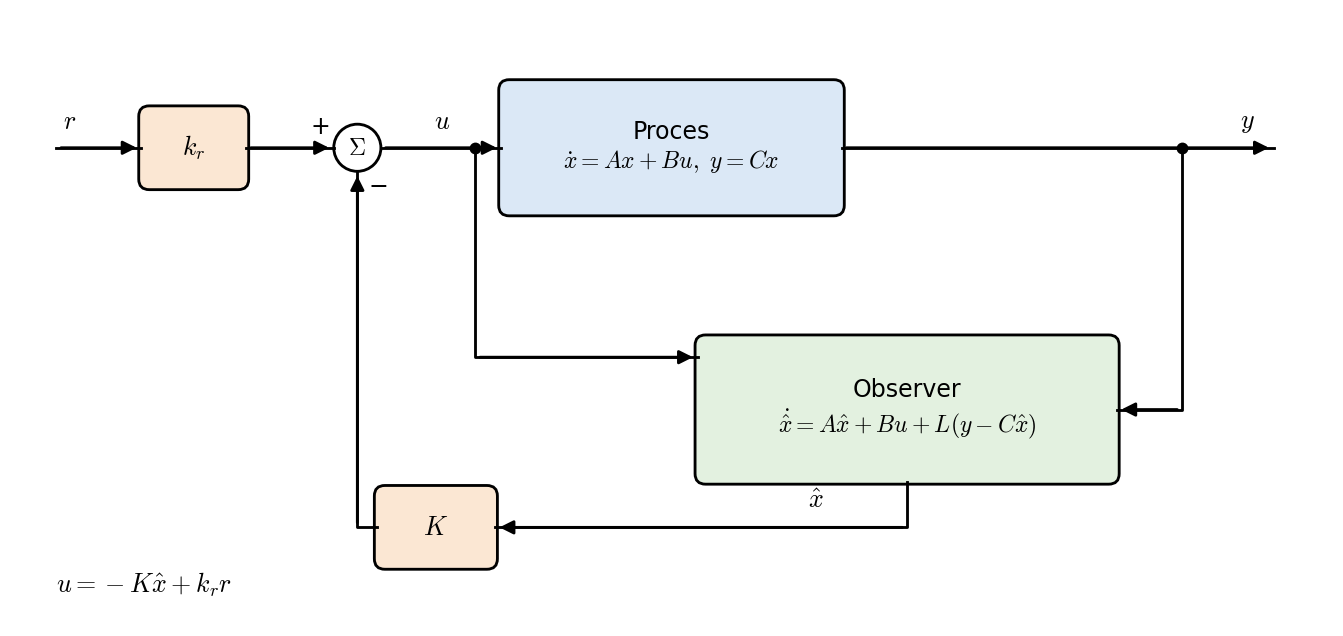
\includegraphics[width=0.8\linewidth,height=\textheight,keepaspectratio,alt={Regulator po izlazima: observer dobija u i y i daje procenu stanja x̂, a zakon upravljanja je u = −K·x̂ + kr·r}]{figures/blok_stanja_observer.png}
\caption{Regulator po izlazima: observer dobija u i y i daje procenu stanja x̂, a zakon upravljanja je u = −K·x̂ + kr·r}
\end{figure}

\textbf{Red regulatora.} Regulator po izlazima ima onoliko stanja koliko observer procenjuje. Red regulatora = red sistema − broj direktno merljivih stanja. Ako se \(x_1 = y\) meri, može se koristiti direktno (\(u = -k_1y - k_2\hat x_2 + k_rr\)), ali predavač \textbf{preporučuje procenjeno \(\hat x_1\)} i kad je \(x_1\) merljivo: merenje nosi šum, a observer ne može da prati šum i brze promene, pa daje osnovnu komponentu signala \izvor{P06 snimak, 16.--20. min}. Tada je red regulatora jednak redu sistema. Pitanje „kog je reda ovaj regulator?'' je postavljeno na času \izvor{P06 snimak, 17.--23. min}.

\begin{ispit}
Pitanja na odbrani domaćeg 3 i 4: zašto \texttt{acker(\allowbreak{}A\textquotesingle{},\allowbreak{}C\textquotesingle{},\allowbreak{}p)\textquotesingle{}} (dualnost), zašto observer brži (separacija važi samo za polove, ali regulator koristi procene), kako je dobijen \(k_r\) i šta se desi sa \(k_r\) ako se promeni \(K\). Proveri \texttt{rank(\allowbreak{}ctrb)} i \texttt{rank(\allowbreak{}obsv)} pre projektovanja. Početni uslovi observera i procesa neka budu različiti, da bi se na grafiku videlo kako \(\hat x \to x\).
\end{ispit}

\section{Estimacija i kompenzacija poremećaja}

\subsection{Ideja}

\textbf{Poremećaj} \(d\) deluje na ulazu procesa, pre njega (npr. opterećenje motora), a \textbf{šum} \(n\) deluje na merenju, posle procesa:

\[u_0 = u + d,\qquad y_0 = y + n .\]

Termini sa predavanja \izvor{P06 snimak, 4.--9. min}: \textbf{pasivni kompenzator} (filter) guši ceo deo spektra, bez obzira na oblik signala; \textbf{aktivni kompenzator} uklanja tačno određen signal poznatog oblika. Šum (mala amplituda, visoka učestanost) se uklanja \textbf{pasivno}, niskopropusnim filtrom \(\frac{1}{T_fs+1}\), koji guši ceo visokofrekventni deo spektra. Poremećaj se uklanja \textbf{aktivno}: procenimo ga (\(\hat d\)) i oduzmemo od upravljanja, \(u = u_{reg} - \hat d\). Tada je \(u_0 = u_{reg} + (d - \hat d) \approx u_{reg}\). Da bismo procenili \(d\), pretpostavimo \textbf{oblik} poremećaja (konstanta, rampa, sinus poznate učestanosti), zapišemo ga kao izlaz malog dinamičkog sistema, \textbf{generatora poremećaja}, i njegova stanja procenjujemo observerom, zajedno sa stanjima procesa.

\subsection{Primer: motor sa poremećajem}

\[\dot x_1 = x_2,\qquad \dot x_2 = -\frac1T x_2 + \frac KT(u + d),\qquad y = x_1 .\]

Tri slučaja:

\begin{enumerate}
\def\labelenumi{\arabic{enumi}.}
\item \(d = 0\), mere se \(x_1\) i \(x_2\): \(u = -k_1x_1 - k_2x_2 + k_rr\).
\item \(d = 0\), meri se samo \(x_1\): observer za \(\hat x_2\), regulator drugog reda.
\item \(d \ne 0\), meri se samo \(x_1\):
  \[u = -k_1\hat x_1 - k_2\hat x_2 + k_rr - \hat d,\]
  \[\dot{\hat x}_1 = \hat x_2 + l_1(y - \hat x_1),\qquad \dot{\hat x}_2 = -\frac1T\hat x_2 + \frac KT(u + \hat d) + l_2(y - \hat x_1),\]
  plus jednačina za \(\hat d\), koja zavisi od oblika poremećaja.
\end{enumerate}

U observeru stoji \(u + \hat d\), jer model mora da opisuje ono što stvarno ulazi u proces.

\subsection{Generator poremećaja}

Poremećaj zamišljamo kao odziv sistema \(D(s)\) na Dirakov impuls. Stanja generatora su \(w\).

\textbf{Konstanta}, \(d = d_0h(t)\), \(D(s) = \frac1s\): sistem prvog reda.

\[\dot w_1 = 0,\qquad d = w_1 .\]

Observer dobija jednu jednačinu više: \(\dot{\hat w}_1 = 0 + l_3(y - \hat x_1)\), \(\hat d = \hat w_1\). Regulator je trećeg reda.

\textbf{Rampa}, \(d = t\,h(t)\), \(D(s) = \frac{1}{s^2}\): izvod rampe je konstanta, a izvod konstante je nula.

\[\dot w_1 = 0,\qquad \dot w_2 = w_1,\qquad d = w_2 .\]

Observer: \(\dot{\hat w}_1 = l_3(y - \hat x_1)\), \(\dot{\hat w}_2 = \hat w_1 + l_4(y - \hat x_1)\). Regulator je četvrtog reda. Konstanta i rampa su oblici poremećaja najavljeni za kurs na prvom predavanju \izvor{P01 snimak, 17.--20. min}.

\textbf{Sinus poznate učestanosti} \(\omega\), nepoznate amplitude i faze. \(D(s) = \frac{1}{s^2 + \omega^2}\), pa \(d\) zadovoljava \(\ddot d = -\omega^2 d\). Izaberemo \(d = w_2\), \(w_1 = \dot w_2\):

\[\dot w_1 = -\omega^2w_2,\qquad \dot w_2 = w_1,\qquad d = w_2 .\]

(U nekim prepisima stoji „\(-w_2W_2\)„; tačno je \(-\omega^2w_2\).) Regulator je četvrtog reda.

\begin{longtable}[]{@{}
  >{\raggedright\arraybackslash}p{(\linewidth - 6\tabcolsep) * \real{0.2105}}
  >{\centering\arraybackslash}p{(\linewidth - 6\tabcolsep) * \real{0.2632}}
  >{\centering\arraybackslash}p{(\linewidth - 6\tabcolsep) * \real{0.2632}}
  >{\centering\arraybackslash}p{(\linewidth - 6\tabcolsep) * \real{0.2632}}@{}}
\caption{Modeli generatora poremećaja, \(\dot w = A_ww\), \(d = C_ww\) (stanja poređana kao \(w = [w_1\;\; w_2]^T\))}\tabularnewline
\toprule\noalign{}
\begin{minipage}[b]{\linewidth}\raggedright
Poremećaj
\end{minipage} & \begin{minipage}[b]{\linewidth}\centering
\(D(s)\)
\end{minipage} & \begin{minipage}[b]{\linewidth}\centering
\(A_w\)
\end{minipage} & \begin{minipage}[b]{\linewidth}\centering
\(C_w\)
\end{minipage} \\
\midrule\noalign{}
\endfirsthead
\toprule\noalign{}
\begin{minipage}[b]{\linewidth}\raggedright
Poremećaj
\end{minipage} & \begin{minipage}[b]{\linewidth}\centering
\(D(s)\)
\end{minipage} & \begin{minipage}[b]{\linewidth}\centering
\(A_w\)
\end{minipage} & \begin{minipage}[b]{\linewidth}\centering
\(C_w\)
\end{minipage} \\
\midrule\noalign{}
\endhead
\bottomrule\noalign{}
\endlastfoot
konstanta & \(\frac1s\) & \(0\) & \(1\) \\
rampa & \(\frac1{s^2}\) & \(\begin{bmatrix}0 & 0\\ 1 & 0\end{bmatrix}\) & \([0\;\;1]\) \\
sinus \(\omega\) & \(\frac{1}{s^2+\omega^2}\) & \(\begin{bmatrix}0 & -\omega^2\\ 1 & 0\end{bmatrix}\) & \([0\;\;1]\) \\
\end{longtable}

U diskretnom vremenu konstanta je \(w(k+1) = w(k)\), tj. \(A_w = 1\) (tako je u referentnom rešenju projekta).

\subsection{Opšti oblik: prošireni observer}

\textbf{Postavka}:

\[\dot x = Ax + B(u + d),\qquad \dot w = A_ww,\qquad d = C_ww,\qquad y = Cx .\]

\textbf{Izvođenje.} Spojimo \(x\) i \(w\) u jedan prošireni vektor stanja. Pošto je \(Bd = BC_ww\):

\[\begin{bmatrix}\dot x\\ \dot w\end{bmatrix} = \underbrace{\begin{bmatrix}A & BC_w\\ 0 & A_w\end{bmatrix}}_{AA}\begin{bmatrix}x\\ w\end{bmatrix} + \underbrace{\begin{bmatrix}B\\ 0\end{bmatrix}}_{BB}u,\qquad y = \underbrace{\begin{bmatrix}C & 0\end{bmatrix}}_{CC}\begin{bmatrix}x\\ w\end{bmatrix}.\]

Za ovaj prošireni sistem pravimo običan observer:

\[\begin{bmatrix}\dot{\hat x}\\ \dot{\hat w}\end{bmatrix} = AA\begin{bmatrix}\hat x\\ \hat w\end{bmatrix} + BB\,u + LL\,(y - C\hat x),\qquad LL = \begin{bmatrix}L\\ L_w\end{bmatrix} = \texttt{acker}(AA', CC', \text{polovi})' .\]

Za Simulink: \(A_o = AA - LL\cdot CC\), \(B_o = [BB\;\; LL]\), \(C_o = I\). Iz izlaza se uzmu \(\hat x\) (prvih \(n\)) i \(\hat d = C_w\hat w\). Upravljanje je

\[u = -K\hat x + k_rr - \hat d .\]

\(K\) i \(k_r\) se računaju kao ranije, samo za \((A, B)\). Observer ima \(n + n_w\) polova, a svi treba da budu brži od regulatora.

Praktični detalji:

\begin{itemize}
\item \textbf{Koje \(u\) ide u observer:} ono koje stvarno ulazi u proces, tj. \(u = u_{reg} - \hat d\) (posle oduzimanja). Model \(AA\) već sam dodaje \(BC_w\hat w\), pa observer tako „vidi'' \(u + \hat d\), kao u primeru sa motorom.
\item \textbf{Polovi:} npr. svih \(n + n_w\) u istoj tački, oko 4 puta brže od regulatora (u primeru ispod regulator \(-2\), observer \(-8\)). \texttt{acker} prima višestruke polove; \texttt{place} traži različite (npr. \(-8, -8{,}5, -9\)). Brži polovi poremećaja daju brže \(\hat d\), ali više šuma u \(\hat d\).
\item \textbf{Diskretno:} generator se diskretizuje tačno, \(A_{w,d} = e^{A_wT_s}\) (\texttt{expm(\allowbreak{}Aw*Ts)}); za konstantu je to \(1\). Proces sa \texttt{c2d}, a polovi observera \(z = e^{pT_s}\).
\item \textbf{Provera:} pre simulacije \texttt{rank(\allowbreak{}obsv(\allowbreak{}AA,\allowbreak{}CC))}; posle simulacije grafik \(d\) i \(\hat d\) (\(\hat d\) treba da stigne \(d\) za vreme reda \(5/q\) za polove u \(-q\)) i grafik \(y\) bez trajne greške.
\end{itemize}

\begin{kljucna}
Prošireni sistem mora biti \textbf{osmotriv}: \texttt{rank(\allowbreak{}obsv(\allowbreak{}AA,\allowbreak{}CC))\ =\ n\ +\ n\_\allowbreak{}w}. Intuicija: poremećaj se „vidi'' samo kroz svoj uticaj na \(y\). Ako bi proces imao nulu tačno na učestanosti poremećaja (npr. nulu u \(s = 0\) za konstantni \(d\)), poremećaj ne bi uticao na izlaz u ustaljenom stanju i ne bi mogao da se proceni.
\end{kljucna}

\textbf{Upozorenje o \(CC\).} Česta greška: \(CC = [C\;\; C_w]\). To odgovara drugom modelu: poremećaj koji se \textbf{dodaje na izlaz} (\(y = Cx + d\)), a ne na ulaz. Tada ni \(AA\) ne sme da ima \(BC_w\) u gornjem desnom bloku. Za poremećaj na ulazu procesa, koji se kompenzuje sa \(u - \hat d\), dosledan izbor je \(AA = \begin{bmatrix}A & BC_w\\ 0 & A_w\end{bmatrix}\) i \(CC = [C\;\; 0]\). Tako rade referentno rešenje domaćeg 4, tvoj \texttt{Vezbe3/\allowbreak{}Observer/\allowbreak{}estimator.m} i referentno rešenje projekta.

Tvoji \texttt{Domaci5} i \texttt{Vezbe3} odstupaju od ovog izbora: vidi mapu domaćih (Domaći 5).

\subsection{Primer i poređenje}

Proces sa slike: \(A = \begin{bmatrix}0 & 1\\ 0 & -2\end{bmatrix}\), \(B = \begin{bmatrix}0\\ 4\end{bmatrix}\), \(C = [1\;\; 0]\), regulator \(K = [1\;\; 0{,}5]\) (polovi \(-2, -2\)), \(k_r = k_1 = 1\), svi polovi observera u \(-8\).

\begin{figure}
\centering
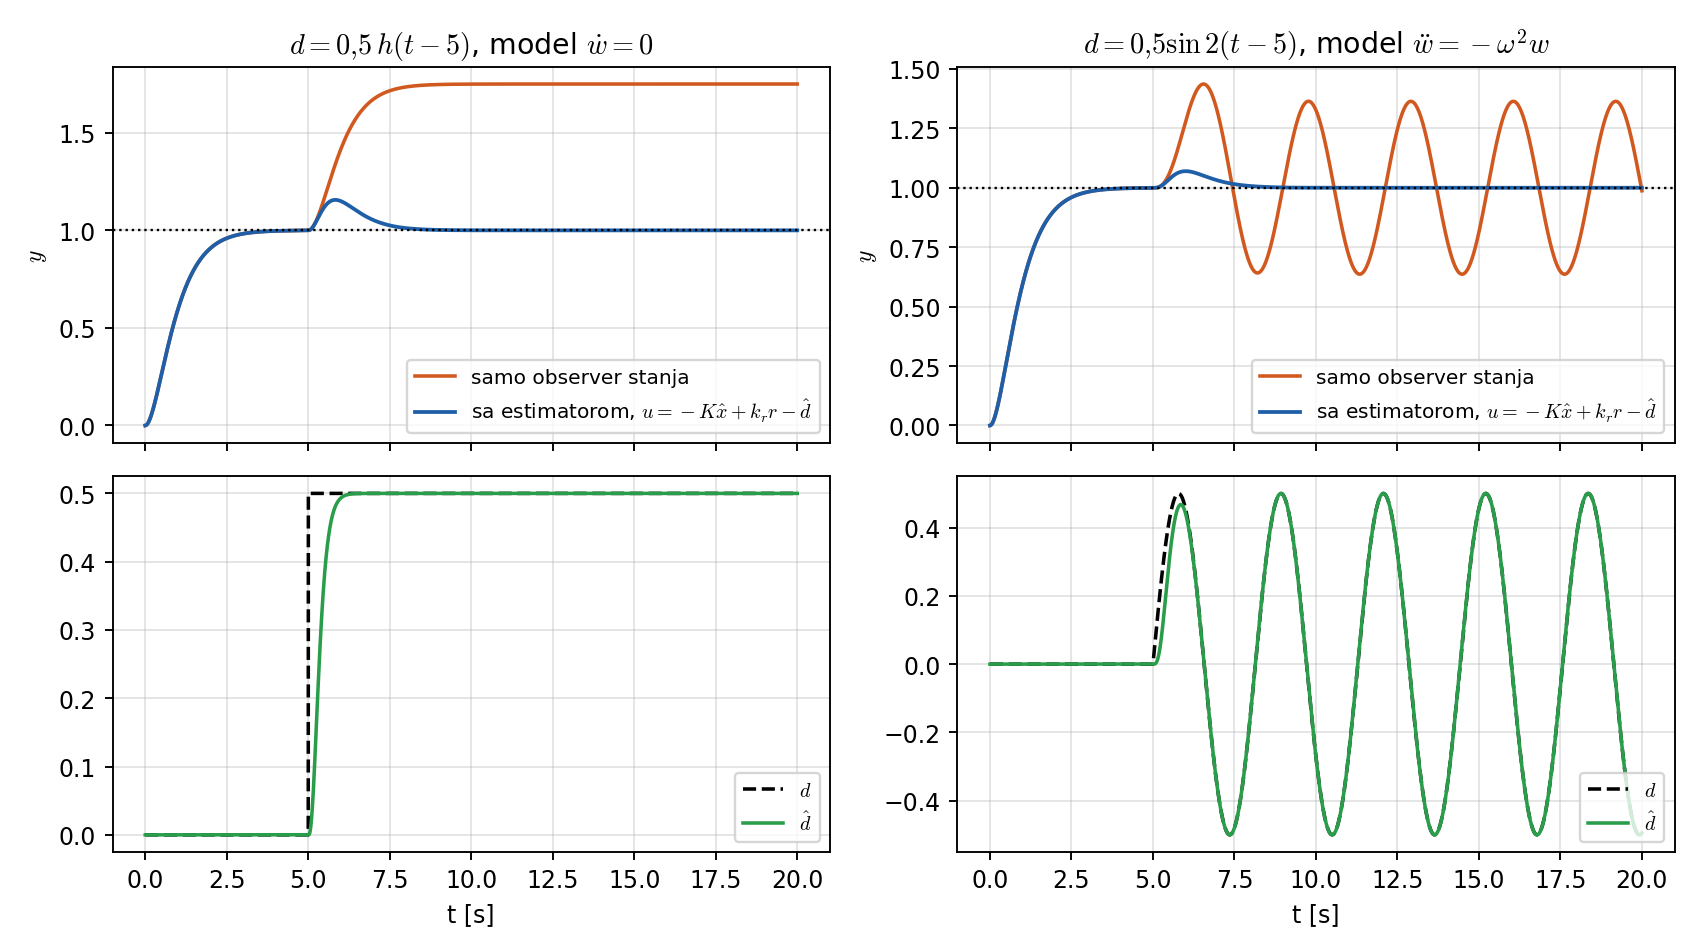
\includegraphics[width=0.95\linewidth,height=\textheight,keepaspectratio,alt={Gore: izlaz sa običnim observerom (narandžasto) i sa proširenim observerom i kompenzacijom u = −K·x̂ + kr·r − d̂ (plavo). Dole: stvarni i procenjeni poremećaj. Levo konstanta, desno sinus. Samo observer stanja ostavlja trajnu grešku, odnosno trajnu oscilaciju; sa modelom poremećaja procena d̂ prati d, a y prati r}]{figures/poremecaj_estimator.png}
\caption{Gore: izlaz sa običnim observerom (narandžasto) i sa proširenim observerom i kompenzacijom u = −K·x̂ + kr·r − d̂ (plavo). Dole: stvarni i procenjeni poremećaj. Levo konstanta, desno sinus. Samo observer stanja ostavlja trajnu grešku, odnosno trajnu oscilaciju; sa modelom poremećaja procena d̂ prati d, a y prati r}
\end{figure}

Zašto bez estimatora ostaje greška? U ustaljenom stanju sa merenim stanjima i konstantnim \(d\): \(\dot x_2 = 0\) i \(x_2 = 0\) daju \(u + d = 0\), tj. \(-k_1x_1 + k_rr = -d\). Odatle je

\[y_{ss} = x_1 = \frac{k_rr + d}{k_1} = r + \frac{d}{k_1}\qquad(k_r = k_1).\]

Greška je \(d/k_1\). Sa estimatorom je \(u + d = -k_1x_1 + k_rr + (d - \hat d)\), a kad \(\hat d \to d\), greška nestaje.

\begin{zasto}
Veza sa integralnim dejstvom: za konstantni poremećaj je \(\dot{\hat w} = l_3(y - \hat x_1)\), tj. \(\hat d\) je \textbf{integral} greške procene izlaza. Estimator konstantnog poremećaja je zato skriveni integrator. Isto kaže i princip unutrašnjeg modela kod RST regulatora (sledeće poglavlje): regulator mora u sebi da ima model poremećaja.
\end{zasto}

\textbf{Kombinovani poremećaj} (konstanta + sinus): generator je zbir, \(A_w = \operatorname{diag}\big(0,\ \begin{bmatrix}0 & -\omega^2\\ 1 & 0\end{bmatrix}\big)\), \(C_w = [1\;\; 0\;\; 1]\). Prošireni sistem je tada reda \(n + 3\).

\begin{ispit}
Za domaći sa estimatorom poremećaja treba znati: razliku poremećaja i šuma, kako se iz \(D(s)\) dobijaju \(A_w\) i \(C_w\), zašto je \(AA\) gornje-trougaona sa \(BC_w\) i zašto \(CC = [C\;\; 0]\), da se \(\hat d\) \textbf{oduzima} od upravljanja, a u observer ulazi \(u + \hat d\). Za sinus mora biti poznata učestanost \(\omega\). Pokazati grafik \(d\) i \(\hat d\) i grafik \(y\) sa i bez kompenzacije.
\end{ispit}

\section{RST regulator}

\subsection{Ideja}

Realni PID ne deluje samo na grešku \(e = r - y\): referenca se množi težinom \(b\), a D dejstvo deluje samo na filtrirani izlaz. Takav regulator je opšti linearni regulator sa \textbf{dva ulaza}, \(r\) i \(y\), sa posebnom funkcijom prenosa za svaki. Zapisan preko tri polinoma, \(R\), \(S\) i \(T\), daje sistematski postupak: polovi zatvorene sprege se postavljaju rešavanjem jedne polinomske (Diofantove) jednačine, a poremećaj se potiskuje tako što se njegov model ugradi u \(R\).

\subsection{Od PID-a do RST strukture}

\textbf{Modifikovano P dejstvo:} \(u_P = K_p(b\,r - y)\). Skok reference daje skok upravljanja, pa se referenca množi sa \(b \le 1\).

\textbf{Modifikovano D dejstvo:} izvod odskočne reference je Dirakov impuls, pa se D deo na referenci izbaci. Izvod izlaza pojačava šum, pa se diferencira filtrirani izlaz:

\[u = K_p(b\,r - y) - K_D\frac{s}{T_fs+1}\,y .\]

Ovde više ne ulazi samo greška. Opšti oblik je

\[u = G_{ff}(s)\,r - G_{fb}(s)\,y,\qquad G_{ff} = \frac{T}{R},\qquad G_{fb} = \frac{S}{R},\]

odnosno, kada se pomnoži sa \(R\):

\[R\,u = T\,r - S\,y .\]

\textbf{Najprostiji primer: modifikovani PI} sa \(b = 0\) \izvor{P07 snimak, 3.--12. min}:

\[u = K_p(0\cdot r - y) + \frac{K_i}{s}(r - y) = \frac{K_i}{s}\,r - \Big(K_p + \frac{K_i}{s}\Big)y .\]

Množenjem sa \(s\): \(s\,u = K_i\,r - (K_ps + K_i)\,y\), pa je \(R = s\), \(T = K_i\), \(S = K_ps + K_i\). Vidi se i da integrator stoji u \(R\). Na predavanju je rečeno da je ovakva struktura „čak mnogo realnija od one tipične'' (sa \(e\) na ulazu).

\begin{figure}
\centering
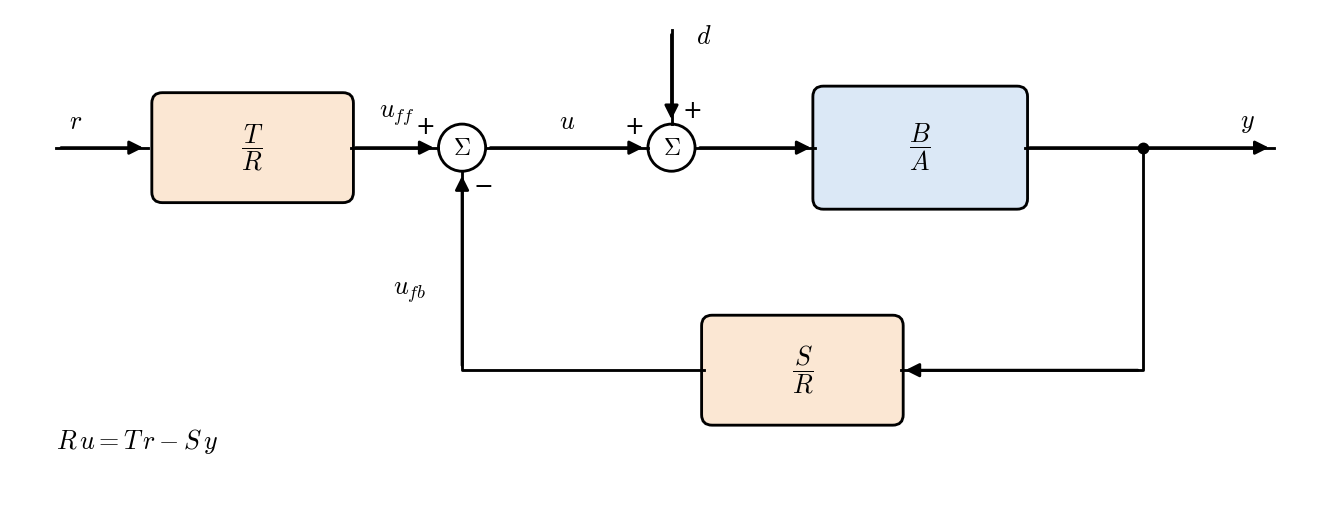
\includegraphics[width=0.85\linewidth,height=\textheight,keepaspectratio,alt={RST struktura: T/R deluje na referencu, S/R na izmereni izlaz, a poremećaj d ulazi pre procesa B/A}]{figures/blok_rst.png}
\caption{RST struktura: T/R deluje na referencu, S/R na izmereni izlaz, a poremećaj d ulazi pre procesa B/A}
\end{figure}

\subsection{Funkcija prenosa zatvorene sprege}

\textbf{Izvođenje} (proces \(y = \frac{B}{A}(u + d)\)):

\begin{enumerate}
\def\labelenumi{\arabic{enumi}.}
\item Iz \(Ru = Tr - Sy\) sledi \(u = \frac{T}{R}r - \frac{S}{R}y\).
\item Zamenimo u \(Ay = B(u + d)\) i pomnožimo sa \(R\): \(ARy = BTr - BSy + BRd\).
\item Članove sa \(y\) prebacimo levo: \((AR + BS)\,y = BT\,r + BR\,d\).
\end{enumerate}

\[y = \frac{BT}{AR + BS}\,r + \frac{BR}{AR + BS}\,d\]

\begin{kljucna}
Karakteristični polinom zatvorene sprege je
\[A_{cl} = AR + BS .\]
Česta greška: u izvođenju ispadne \(AR - SB\) (greška u znaku pri prebacivanju \(-ySB\) na levu stranu). Ispravno je, npr. za \(A = s(s+1)\), \(B = 1\): \(f_{cl} = s(s+1)R + S\). Sa znakom minus bi svi dobijeni koeficijenti \(S\) imali pogrešan znak.
\end{kljucna}

Iz izraza se vidi podela uloga:

\begin{itemize}
\item \(R\) i \(S\) određuju \textbf{polove} (\(A_{cl}\)), dakle stabilnost i brzinu;
\item \(R\) je u \textbf{brojiocu} prenosa od \(d\) do \(y\), pa \(R\) potiskuje poremećaj;
\item \(T\) utiče samo na referencu, pa se bira za jedinično statičko pojačanje.
\end{itemize}

\subsection{Postupak projektovanja}

\begin{enumerate}
\def\labelenumi{\arabic{enumi}.}
\item \textbf{Zadamo željeni polinom} \(A_{cl}^*\), npr. sve polove u \(-p\): \((s + p)^{n_{cl}}\).
\item \textbf{Izaberemo stepene} \(R\) i \(S\):

  \begin{itemize}
  \tightlist
  \item \(R\) je moni (vodeći koeficijent 1), jer se \(R\), \(S\) i \(T\) mogu podeliti istim brojem;
  \item \(\deg S \le \deg R\), da bi \(S/R\) bio kauzalan;
  \item broj nepoznatih koeficijenata mora biti jednak broju koeficijenata \(A_{cl}\) koje treba izjednačiti.
  \end{itemize}
\item \textbf{Rešimo Diofantovu jednačinu} \(AR + BS = A_{cl}^*\) izjednačavanjem koeficijenata uz iste stepene \(s\). Jednačina je \textbf{linearna} po koeficijentima \(R\) i \(S\).
\item \textbf{Odredimo \(T\)} (konstanta) iz uslova \(\lim_{s\to 0}\frac{BT}{A_{cl}} = 1\):
  \[T = \frac{A_{cl}(0)}{B(0)},\qquad\text{diskretno}\qquad T = \frac{A_{cl}(1)}{B(1)} .\]
\end{enumerate}

\textbf{Brojanje stepeni.} Neka je \(\deg A = n\), \(R\) moni stepena \(n_R\) i \(\deg S = n_R\). Nepoznatih je \(n_R + (n_R + 1)\), a \(A_{cl}\) je stepena \(n + n_R\) i moni, pa ima \(n + n_R\) slobodnih koeficijenata. Iz \(2n_R + 1 = n + n_R\) sledi

\[n_R = n - 1 \qquad(\text{bez modela poremećaja}).\]

Za proces 2. reda \(R\) je 1. stepena, za proces 3. reda 2. stepena. Izvori to rade „pokušajima'' (pokušaj sa \(R = 1\) ne uspe, pa se podiže stepen), a pravilo daje isti rezultat. Primer sa predavanja \izvor{P07 snimak, 35.--39. min}, \(\frac{1}{(s+1)^3}\) (\(n = 3\)): \(R\) 1. stepena i \(S\) 1. stepena daju \(A_{cl}\) 4. reda, a samo 3 parametra, pa ne ide; \(R\) 2. stepena i \(S\) 2. stepena daju \(A_{cl}\) 5. reda i \(2 + 3 = 5\) parametara, pa ide (\(n_R = n - 1 = 2\)).

\textbf{Uslov rešivosti.} Diofantova jednačina ima rešenje za proizvoljan \(A_{cl}^*\) ako \(A\) i \(B\) \textbf{nemaju zajednički koren} (proces nema skraćivanje pola i nule). To je polinomski oblik uslova upravljivosti.

\subsection{\texorpdfstring{Primer: \(G(s) = \dfrac{1}{s(s+1)}\)}{Primer: G(s) = \textbackslash dfrac\{1\}\{s(s+1)\}}}

\(A = s(s+1)\), \(B = 1\), \(n = 2\), pa je \(R = s + \sigma\), \(S = \rho_1 s + \rho_0\).

\begin{enumerate}
\def\labelenumi{\arabic{enumi}.}
\item \(AR + BS = (s^2 + s)(s + \sigma) + \rho_1s + \rho_0 = s^3 + (1 + \sigma)s^2 + (\sigma + \rho_1)s + \rho_0\).
\item Željeno \((s + p)^3 = s^3 + 3ps^2 + 3p^2s + p^3\).
\item Izjednačavanje: \(1 + \sigma = 3p\), \(\sigma + \rho_1 = 3p^2\), \(\rho_0 = p^3\).
\item Za \(p = 1\): \(\sigma = 2\), \(\rho_1 = 1\), \(\rho_0 = 1\).
\item \(T = A_{cl}(0)/B(0) = \rho_0 = 1\).
\end{enumerate}

Regulator \(S/R = \frac{\rho_1s + \rho_0}{s + \sigma}\) je PD sa filtriranim D dejstvom na izlazu. Pokušaj sa \(R = 1\), \(S = \rho\) (P regulator) daje \(s^2 + s + \rho\): dva koeficijenta, jedan parametar, pa ne može.

\subsection{Potiskivanje poremećaja: princip unutrašnjeg modela}

\textbf{Cilj:} za \(r = 0\) poremećaj ne sme da ostavi trag na izlazu u ustaljenom stanju. Po teoremi o konačnoj vrednosti:

\[y_{ss} = \lim_{s\to 0} s\,\frac{B(s)R(s)}{A_{cl}(s)}\,D(s) = 0 .\]

\textbf{Konstanta}, \(D = \frac{d_0}{s}\): \(y_{ss} = \frac{B(0)R(0)}{A_{cl}(0)}d_0\). Nula je ako i samo ako je \(R(0) = 0\), tj. \(R\) sadrži faktor \(s\). To je \textbf{integrator u regulatoru} (pol regulatora \(S/R\) u nuli). U svesci piše „\(R\) mora sadržati pol u \((0,0)\)„, što znači upravo ovo.

\textbf{Rampa}, \(D = \frac{1}{s^2}\): jedan \(s\) iz \(R\) se skrati sa \(s\) iz limesa, za drugi treba još jedan, pa \(R\) sadrži \(s^2\).

\textbf{Sinus}, \(D = \frac{\omega}{s^2 + \omega^2}\): da bi se imenilac skratio, \(R\) mora da sadrži \(s^2 + \omega^2\). U svesci piše „u \(R\) ide \(1/\mathcal L\{d\}\) otprilike''. Tačnije je: u \(R\) ide \textbf{imenilac} transformacije poremećaja, a brojilac nije bitan.

\begin{kljucna}
\textbf{Princip unutrašnjeg modela:} \(R = D_d\cdot R_1\), gde je \(D_d\) imenilac modela poremećaja. Regulator u sebi ima generator tog signala, pa sam može da proizvede \(u \to -d\). \(R_1\) je moni i služi da broj parametara bude dovoljan. Rečenica sa predavanja: „\(R\) uvek treba da sadrži imenilac modela poremećaja koji hoćete da potisnete'' \izvor{snimak Mirna pred snimak1\_1, 0. min}.
\end{kljucna}

\begin{zasto}
Zašto ne bi bio dovoljan filter sa polom „blizu \(\omega\)„? Faktor \(s^2 + \omega^2\) u \(R\) daje regulatoru \textbf{beskonačno pojačanje tačno na \(\omega\)}, pa prenos \(d \to y\) (sa \(R\) u brojiocu) ima nulu baš tu i sinus potpuno nestaje. Pol blizu \(\omega\) daje samo konačno pojačanje, pa ostaje oscilacija manje amplitude. Na predavanju je to nazvano „notch'' koji „čupa samo tu frekvenciju'' \izvor{P07 snimak, 52.--60. min}.
\end{zasto}

\begin{longtable}[]{@{}
  >{\raggedright\arraybackslash}p{(\linewidth - 4\tabcolsep) * \real{0.2857}}
  >{\centering\arraybackslash}p{(\linewidth - 4\tabcolsep) * \real{0.3571}}
  >{\centering\arraybackslash}p{(\linewidth - 4\tabcolsep) * \real{0.3571}}@{}}
\caption{Faktor koji \(R\) mora da sadrži}\tabularnewline
\toprule\noalign{}
\begin{minipage}[b]{\linewidth}\raggedright
Poremećaj
\end{minipage} & \begin{minipage}[b]{\linewidth}\centering
kontinualno \(D_d(s)\)
\end{minipage} & \begin{minipage}[b]{\linewidth}\centering
diskretno \(D_d(z)\)
\end{minipage} \\
\midrule\noalign{}
\endfirsthead
\toprule\noalign{}
\begin{minipage}[b]{\linewidth}\raggedright
Poremećaj
\end{minipage} & \begin{minipage}[b]{\linewidth}\centering
kontinualno \(D_d(s)\)
\end{minipage} & \begin{minipage}[b]{\linewidth}\centering
diskretno \(D_d(z)\)
\end{minipage} \\
\midrule\noalign{}
\endhead
\bottomrule\noalign{}
\endlastfoot
konstanta & \(s\) & \(z - 1\) \\
rampa & \(s^2\) & \((z-1)^2\) \\
sinus \(\omega\) & \(s^2 + \omega^2\) & \(z^2 - 2\cos(\omega T_s)z + 1\) \\
konstanta + sinus & \(s(s^2 + \omega^2)\) & \((z-1)(z^2 - 2\cos(\omega T_s)z + 1)\) \\
više sinusa \(\omega_1, \omega_2, \omega_3\) & \(\prod_i (s^2 + \omega_i^2)\) & \(\prod_i (z^2 - 2\cos(\omega_i T_s)z + 1)\) \\
periodičan, perioda \(N\) odbiraka & --- & \(z^N - 1\) \\
\end{longtable}

Diskretni sinus: polovi signala \(\sin(\omega kT_s)\) su \(e^{\pm j\omega T_s}\), pa je \((z - e^{j\omega T_s})(z - e^{-j\omega T_s}) = z^2 - 2\cos(\omega T_s)z + 1\). Česta greška (viđena i na času \izvor{P07 snimak, 62. min}): za konstantu u diskretnom slučaju reći „1'' umesto \(z - 1\); konstanti odgovara pol \(z = 1\), pa u \(R\) ide faktor \(z - 1\).

\textbf{Brojanje stepeni sa poremećajem.} Nepoznati su koeficijenti \(R_1\) (moni, stepena \(n_{R1}\)) i \(S\) (stepena \(\deg R\)). Isti račun kao gore daje \(n_{R1} = n - 1\), \textbf{nezavisno od poremećaja}. Za \(1/(s(s+1))\) je uvek \(R_1 = s + \sigma\).

\textbf{Primer: \(G = \frac{1}{s(s+1)}\), \(d\) = konstanta, svi polovi u \(-2\).}

\begin{enumerate}
\def\labelenumi{\arabic{enumi}.}
\item \(R = s(s + \sigma)\), \(S = \rho_2s^2 + \rho_1s + \rho_0\): 4 nepoznate, \(A_{cl}\) 4. reda.
\item \(AR = s^2(s+1)(s+\sigma) = s^4 + (1+\sigma)s^3 + \sigma s^2\).
\item \(AR + BS = s^4 + (1+\sigma)s^3 + (\sigma + \rho_2)s^2 + \rho_1s + \rho_0\).
\item \((s+2)^4 = s^4 + 8s^3 + 24s^2 + 32s + 16\).
\item \(\sigma = 7\), \(\rho_2 = 17\), \(\rho_1 = 32\), \(\rho_0 = 16\), \(T = 16\).
\end{enumerate}

Isti primer je rađen na predavanju \izvor{P07 snimak, 65.--75. min}, u opštem obliku: za \(A_{cl}^* = s^4 + a_3s^3 + a_2s^2 + a_1s + a_0\) je \(\sigma = a_3 - 1\), \(\rho_2 = a_2 - \sigma\), \(\rho_1 = a_1\), \(\rho_0 = a_0\), \(T = a_0\), dakle rešenje u zatvorenom obliku, bez \texttt{solve}. Željeni polinom se u MATLAB-u dobija sa \texttt{poly(\allowbreak{}{[}-2\ -2\ -2\ -2{]})} ili ugnežđenim \texttt{conv(\allowbreak{}{[}1\ 2{]},\allowbreak{}{[}1\ 2{]})}, što daje \texttt{{[}1\ 8\ 24\ 32\ 16{]}}.

\textbf{Isti proces, \(d = \sin 2t\)}, polovi u \(-2\): \(R = (s^2+4)(s+\sigma)\), \(S\) 3. stepena, \(A_{cl}\) 5. reda. Proverimo rešenje \(\sigma = 9\), \(S = 27s^3 + 40s^2 + 44s + 32\):

\[(s^2+s)(s^3 + 9s^2 + 4s + 36) = s^5 + 10s^4 + 13s^3 + 40s^2 + 36s,\]

\[AR + BS = s^5 + 10s^4 + 40s^3 + 80s^2 + 80s + 32 = (s+2)^5 .\]

Tačno. \(T = 32\). Za konstantu + sinus: \(R = s(s^2+4)(s+11)\), \(S = 45s^4 + 112s^3 + 196s^2 + 192s + 64\), \(T = 64\).

\begin{figure}
\centering
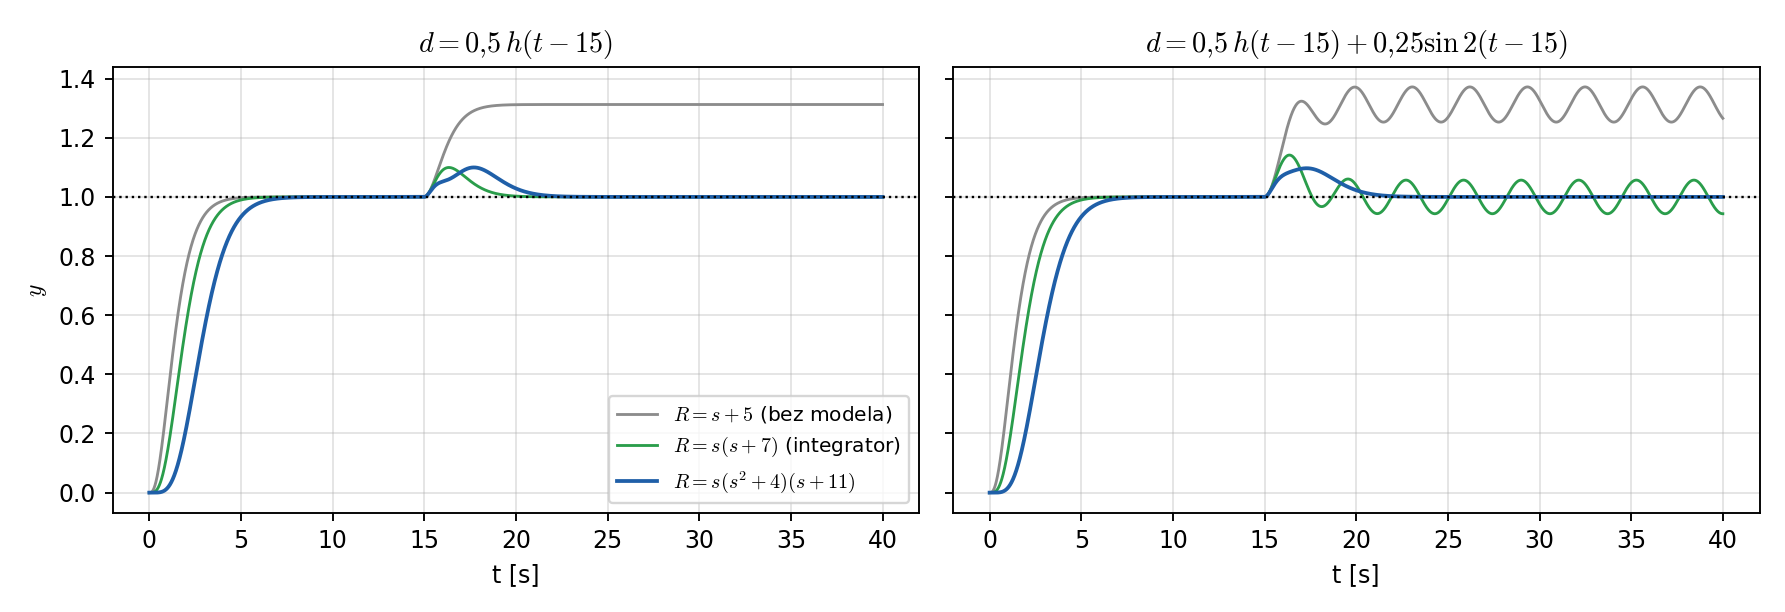
\includegraphics[width=0.95\linewidth,height=\textheight,keepaspectratio,alt={Isti proces 1/(s(s+1)) sa tri RST regulatora. Bez modela poremećaja ostaje trajna greška σ·d0/ρ0 = 5·0,5/8 ≈ 0,31. Sa integratorom nestaje konstanta, ali ostaje sinus. Sa modelom s(s² + 4) potiskuju se oba}]{figures/rst_poremecaj.png}
\caption{Isti proces 1/(s(s+1)) sa tri RST regulatora. Bez modela poremećaja ostaje trajna greška σ·d0/ρ0 = 5·0,5/8 ≈ 0,31. Sa integratorom nestaje konstanta, ali ostaje sinus. Sa modelom s(s² + 4) potiskuju se oba}
\end{figure}

Zanimljivo: proces već ima integrator, pa referenca nema grešku ni bez modela. Za poremećaj koji ulazi \textbf{pre} tog integratora to ne pomaže. Integrator mora biti u regulatoru, tj. u \(R\).

\subsection{Kontinualni i diskretni RST}

\begin{longtable}[]{@{}
  >{\raggedright\arraybackslash}p{(\linewidth - 4\tabcolsep) * \real{0.2157}}
  >{\raggedright\arraybackslash}p{(\linewidth - 4\tabcolsep) * \real{0.3039}}
  >{\raggedright\arraybackslash}p{(\linewidth - 4\tabcolsep) * \real{0.4804}}@{}}
\caption{Poređenje kontinualnog i diskretnog RST projektovanja}\tabularnewline
\toprule\noalign{}
\begin{minipage}[b]{\linewidth}\raggedright
\end{minipage} & \begin{minipage}[b]{\linewidth}\raggedright
kontinualno
\end{minipage} & \begin{minipage}[b]{\linewidth}\raggedright
diskretno
\end{minipage} \\
\midrule\noalign{}
\endfirsthead
\toprule\noalign{}
\begin{minipage}[b]{\linewidth}\raggedright
\end{minipage} & \begin{minipage}[b]{\linewidth}\raggedright
kontinualno
\end{minipage} & \begin{minipage}[b]{\linewidth}\raggedright
diskretno
\end{minipage} \\
\midrule\noalign{}
\endhead
\bottomrule\noalign{}
\endlastfoot
promenljiva & \(s\) & \(z\) \\
stabilni polovi & leva poluravan & unutar jediničnog kruga \\
željeni polovi & \((s + p)^n\) & \((z - z_p)^n\), \(z_p = e^{-pT_s}\) \\
statičko pojačanje & \(s \to 0\): \(T = A_{cl}(0)/B(0)\) & \(z \to 1\): \(T = A_{cl}(1)/B(1)\) \\
konstanta u \(R\) & \(s\) & \(z - 1\) \\
kauzalnost & \(\deg S \le \deg R\) & \(\deg S \le \deg R\) (jednako: \(u(k)\) zavisi od \(y(k)\)) \\
\end{longtable}

\textbf{Diskretni primer:} \(G(z) = \dfrac{0{,}1}{(z+0{,}3)^2}\), \(d(k) = k\,h(k)\) (rampa). \(R = (z-1)^2(z + \sigma_0)\), \(S = \rho_3z^3 + \rho_2z^2 + \rho_1z + \rho_0\): 5 nepoznatih, \(A_{cl}\) 5. reda. Z-transformacija rampe \(kT_s\) je \(\frac{T_sz}{(z-1)^2}\). U svesci piše \(T(z)\), ali \(T\) je tu perioda odabiranja, ne polinom \(T\).

\textbf{Deadbeat polovi.} U diskretnom slučaju polovi u \(z = 0\) su najbrži mogući. Kod visokog reda (npr. periodični poremećaj \(z^8 - 1\)) dobija se ogromno upravljanje (\(|u|\) do 1044) kada se svih 11 polova stavi u 0,5, a razumno (\(|u| \approx 18\)) sa 3 pola u 0,5 i 8 u nuli. Pouka: gledati i \(u\), ne samo \(y\).

\subsection{Rešavanje u MATLAB-u}

Za viši red koeficijente je lakše dobiti u MATLAB-u. Dva načina iz referentnih rešenja:

\begin{itemize}
\item \textbf{simbolički} (tvoj \texttt{rst.m}): \texttt{syms\ s\ sigma\ ro\_\allowbreak{}2\ ro\_\allowbreak{}1\ ro\_\allowbreak{}0}, \texttt{f\_\allowbreak{}cl\ =\ expand(\allowbreak{}A*R\ +\ B*S)}, \texttt{solve(\allowbreak{}coeffs(\allowbreak{}f\_\allowbreak{}cl,\allowbreak{}s,\allowbreak{}\textquotesingle{}All\textquotesingle{})\ ==\ coeffs(\allowbreak{}(\allowbreak{}s+p)\^{}n,\allowbreak{}s,\allowbreak{}\textquotesingle{}All\textquotesingle{}))};
\item \textbf{linearni sistem}: izjednačavanje koeficijenata je \(Mx = b\), pa \texttt{x\ =\ M\textbackslash{}b} (referentno rešenje \texttt{domaci5\_\allowbreak{}2\_\allowbreak{}k.m}).
\end{itemize}

Posle toga: \texttt{Gff\ =\ tf(\allowbreak{}T,\allowbreak{}\ R)}, \texttt{Gfb\ =\ tf(\allowbreak{}S,\allowbreak{}\ R)} i u Simulinku \(u = G_{ff}r - G_{fb}y\). Pošto \(R\) sada ima korene na imaginarnoj osi (integrator, sinus), \(G_{ff}\) i \(G_{fb}\) \textbf{same po sebi} nisu stabilne. To je u redu, jer je stabilna zatvorena sprega.

\textbf{Na predavanju} je RST napravljen baš kao \textbf{dva odvojena bloka} \emph{Transfer Fcn}, \texttt{T/R} na referenci i \texttt{S/R} na izlazu, sa sabiračem sa minusom, i u simulaciji je radilo: poremećaj uključen u 4. s je „odmah oboren'' \izvor{P07 snimak, 79.--84. min}. To radi jer se rastući unutrašnji signali dva bloka (npr. integral od \(r\) i integral od \(y\)) poništavaju u razlici. Čistije je ipak jedan blok \(R u = Tr - Sy\) (zajednički \(1/R\)): kod dugih simulacija ili na pravom kontroleru dva nezavisna nestabilna bloka mogu da „pobegnu'' numerički. Na odbrani umeti objasniti oba.

Kako napraviti taj jedan blok: regulator je sistem sa dva ulaza, \([r;\ y]\), i jednim izlazom \(u\). U MATLAB-u \texttt{Kreg\ =\ minreal(\allowbreak{}ss(\allowbreak{}{[}tf(\allowbreak{}T,\allowbreak{}R),\allowbreak{}\ -tf(\allowbreak{}S,\allowbreak{}R){]}))} daje minimalnu realizaciju u kojoj oba ulaza dele ista stanja, pa se nestabilni modovi iz \(R\) ne dupliraju. Matrice \texttt{Kreg.A,\allowbreak{}\ Kreg.B,\allowbreak{}\ Kreg.C,\allowbreak{}\ Kreg.D} idu u blok \emph{State-Space}, a ulazi se spoje sa \emph{Mux} redom \([r;\ y]\). Diskretno: \texttt{tf(\allowbreak{}T,\allowbreak{}R,\allowbreak{}Ts)} i blok \emph{Discrete State-Space} sa istim \(T_s\). Za diskretni RST proces se diskretizuje sa \texttt{c2d(\allowbreak{}G,\allowbreak{}\ Ts)} (ZOH), a \(A(z)\) i \(B(z)\) su imenilac i brojilac rezultata. Zašto ZOH, a ne Tustin: proces iza D/A konvertora stvarno vidi upravljanje koje je konstantno između odbiraka, pa je ZOH tačan ekvivalent; Tustin se koristi za diskretizaciju regulatora i filtara („to ti je proces, nije filter'') \izvor{P07 snimak, 84.--87. min}.

\textbf{Kako izabrati polove \(A_{cl}^*\).} \(A_{cl}\) je višeg reda od procesa (npr. 3. reda za proces 2. reda). Korisno je gledati ga kao proizvod: \(n\) „glavnih'' polova, koji određuju brzinu odziva (biraju se kao kod regulatora po stanjima), i ostatak, koji igra ulogu polova observera i stavlja se 3 do 5 puta dalje (standardna praksa, nije rečeno na predavanju; tamo je samo rečeno da RST „ima observer u sebi'' \izvor{P07 snimak, 38. min}). \textbf{Na predavanju} su svi polovi stavljani u istu tačku, što takođe radi (primeri iznad), ali tada ceo odziv diktira ta jedna brzina: polovi u \(-5\) smiruju odziv za oko 2 s, u \(-2\) za oko 5 s, a \(-1\) je „previše spor''; brži polovi brže potiskuju i poremećaj \izvor{P07 snimak, 79.--82. min}.

\textbf{Kako proveriti.} \texttt{roots(\allowbreak{}conv(\allowbreak{}A,\allowbreak{}R)\ +\ {[}0\ conv(\allowbreak{}B,\allowbreak{}S){]})} (dopuniti nulama na istu dužinu) mora dati zadate polove. Zatim simulacija: \(y\) prati \(r\) bez trajne greške, posle uključenja poremećaja \(y\) se vraća na \(r\), i \(u\) je razumne veličine.

\begin{ispit}
Na odbrani RST domaćeg: izvesti \(y/r = BT/(AR + BS)\) i \(y/d = BR/(AR + BS)\), objasniti zašto \(R\) mora da sadrži imenilac poremećaja (skraćivanje u limesu), prebrojati parametre i red, izračunati \(T\) iz statičkog pojačanja. Zamka: znak u \(A_{cl}\) (\(AR + BS\), ne \(AR - BS\)). Za sinus mora biti poznata učestanost. Pokazati grafik bez modela poremećaja (trajna greška) i sa njim.

Domaći sa predavanja \izvor{P07 snimak, 83.--84. min}: za „vaš'' motor \(\frac{K}{s(Ts+1)}\) napraviti RST koji potiskuje \textbf{konstantan + sinusni} poremećaj (\(R = s(s^2 + \omega^2)R_1\)), a diskretno kao dodatak (\texttt{c2d}, ZOH).
\end{ispit}

\section{Uvod u adaptivno upravljanje}

\subsection{Ideja}

Do sada je postupak bio: dobijemo model (npr. parametri 3, 6, 9), projektujemo regulator za taj model, simuliramo i sve radi. U stvarnom sistemu parametri se \textbf{menjaju} (habanje, temperatura, opterećenje, masa tereta). Posle nekog vremena nisu više 3, 6, 9 nego 4, 7, 8, a polovi koje smo podesili više nisu tamo gde smo ih stavili. \textbf{Adaptivni} regulator ima podesive parametre i jasno definisan algoritam koji ih menja u realnom vremenu, prema promenama u procesu. Primer sa prvog predavanja: tempomat projektovan za auto sa jednim putnikom radi, a sa pet putnika i punim gepekom parametri modela su drugi (npr. \(\frac{3}{s+2}\) postaje \(\frac{4}{s+1}\)), pa treba ponovo izračunati regulator, estimator stanja i estimator poremećaja \izvor{P01 snimak, 13.--18. min}.

\subsection{Pristupi}

\textbf{Gain scheduling} (najjednostavniji). Za nekoliko radnih tačaka (npr. referenca 1, 10, 20) model se linearizuje, projektuje se regulator i parametri se upišu u tabelu. Regulator u radu gleda radnu tačku i čita parametre iz tabele. Između dve radne tačke uzima se najbliža ili se interpolira. Na snimku je primer: za proces \(\frac{3}{s+2}\) projektuje se PID, pa još dva PID-a za slučajeve kada je pojačanje 6 i 10, i regulator se prebacuje (switch) između tri podešavanja prema tome u kom je režimu proces \izvor{P08 snimak, 3.--5. min}. Mana: pokriva samo promene koje su unapred predviđene i izmerene.

\textbf{Autotuning.} Parametri se podese automatski jednim eksperimentom (npr. relejni test za PID), pa ostaju fiksni do sledećeg podešavanja.

\textbf{Pravo adaptivno upravljanje} podešava parametre stalno. Takav sistem ima \textbf{dve petlje}: glavnu (regulator i proces) i petlju adaptacije, koja podešava regulator \izvor{P08 snimak, 9.--10. min}. Dve grupe:

\begin{longtable}[]{@{}
  >{\raggedright\arraybackslash}p{(\linewidth - 4\tabcolsep) * \real{0.2231}}
  >{\raggedright\arraybackslash}p{(\linewidth - 4\tabcolsep) * \real{0.4050}}
  >{\raggedright\arraybackslash}p{(\linewidth - 4\tabcolsep) * \real{0.3719}}@{}}
\caption{Direktno i indirektno adaptivno upravljanje}\tabularnewline
\toprule\noalign{}
\begin{minipage}[b]{\linewidth}\raggedright
\end{minipage} & \begin{minipage}[b]{\linewidth}\raggedright
Direktno
\end{minipage} & \begin{minipage}[b]{\linewidth}\raggedright
Indirektno
\end{minipage} \\
\midrule\noalign{}
\endfirsthead
\toprule\noalign{}
\begin{minipage}[b]{\linewidth}\raggedright
\end{minipage} & \begin{minipage}[b]{\linewidth}\raggedright
Direktno
\end{minipage} & \begin{minipage}[b]{\linewidth}\raggedright
Indirektno
\end{minipage} \\
\midrule\noalign{}
\endhead
\bottomrule\noalign{}
\endlastfoot
Šta se procenjuje & direktno parametri regulatora & parametri \textbf{procesa} \\
Kako se menja regulator & mehanizam adaptacije menja regulator na osnovu greške & iz procena se regulator \textbf{ponovo projektuje} \\
Model procesa & ne računa se eksplicitno & eksplicitno se identifikuje \\
Primer & MRAC sa MIT pravilom & RLS + \texttt{acker} (projekat) \\
\end{longtable}

\begin{figure}
\centering
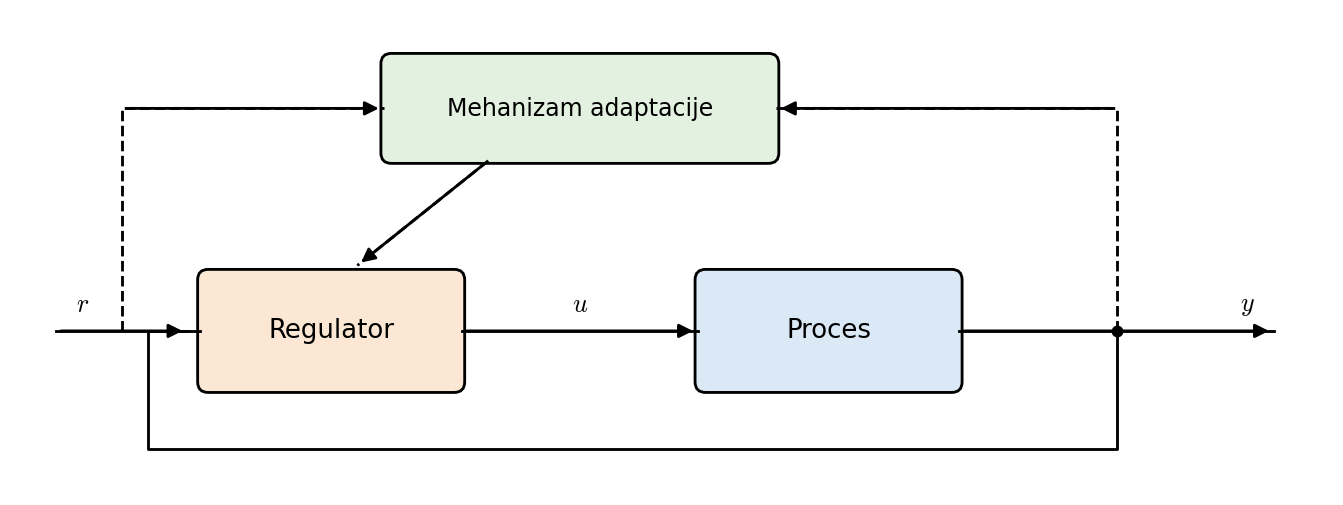
\includegraphics[width=0.8\linewidth,height=\textheight,keepaspectratio,alt={Direktno adaptivno upravljanje: mehanizam adaptacije posmatra referencu, upravljanje i izlaz i direktno podešava regulator}]{figures/blok_direktno.png}
\caption{Direktno adaptivno upravljanje: mehanizam adaptacije posmatra referencu, upravljanje i izlaz i direktno podešava regulator}
\end{figure}

\begin{figure}
\centering
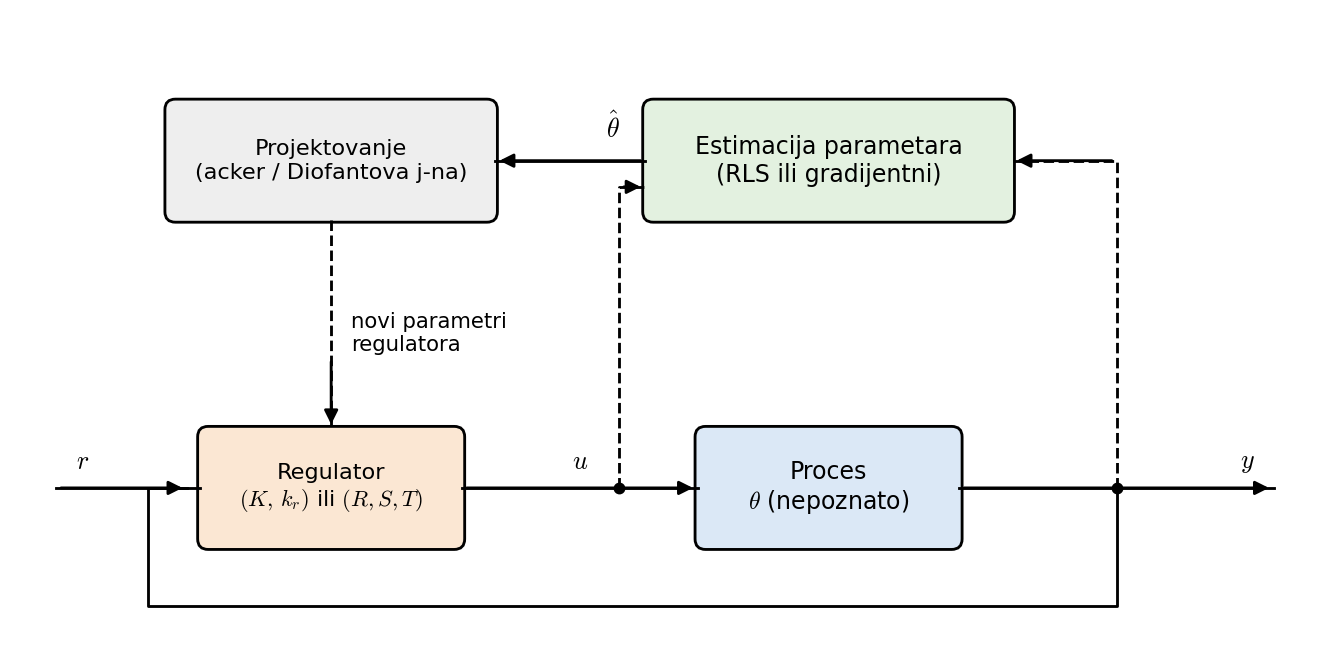
\includegraphics[width=0.8\linewidth,height=\textheight,keepaspectratio,alt={Indirektno adaptivno upravljanje: estimator iz u i y računa procenu θ̂, a blok za projektovanje iz nje računa nove parametre regulatora}]{figures/blok_indirektno.png}
\caption{Indirektno adaptivno upravljanje: estimator iz u i y računa procenu θ̂, a blok za projektovanje iz nje računa nove parametre regulatora}
\end{figure}

Na kursu se radi \textbf{indirektno} adaptivno upravljanje, i to je tema završnog projekta.

\subsection{Primer ideje}

Proces \(\frac{a}{s + b}\) i regulator čiji parametar sledi iz nekog pravila projektovanja, npr. \(K_p = f(a, b)\) (u svesci je kao ilustracija napisano \(K_p = a/b\)). U svakom trenutku:

\begin{enumerate}
\def\labelenumi{\arabic{enumi}.}
\item iz merenja \(u\) i \(y\) procenimo \(\hat a(t)\) i \(\hat b(t)\);
\item izračunamo \(K_p = f(\hat a, \hat b)\);
\item primenimo taj regulator.
\end{enumerate}

Isto za regulator po stanjima: \(K = \texttt{acker}(A(\hat\theta), B(\hat\theta), \text{polovi})\). Kada se procene promene, ponovo se zove \texttt{acker}.

\subsection{Princip izvesne ekvivalencije}

\begin{kljucna}
\textbf{Certainty equivalence:} regulator se projektuje \textbf{kao da su trenutne procene tačne}, tj. \(\hat\theta\) se ubaci u formule umesto \(\theta\). Nesigurnost procene se ne uzima u obzir. To je osnova indirektnog adaptivnog upravljanja.
\end{kljucna}

Posledice koje treba znati na odbrani:

\begin{itemize}
\item \textbf{Struktura regulatora je fiksna}, menjaju se samo parametri. Struktura modela (red, integrator) se ne procenjuje, nego se zna unapred.
\item Kvalitet upravljanja zavisi od kvaliteta procene. Male greške procene obično ne smetaju, jer je regulator dovoljno robustan („regulator pegla svašta'' \izvor{P09 snimak, 53.--54. i 67. min}). Velike greške (npr. \(\hat b \to 0\)) daju loš regulator, a u najgorem slučaju nestabilnu petlju.
\item \textbf{Pobuda.} Procena napreduje samo kad signali nose informaciju. U zatvorenoj sprezi sa konstantnom referencom, posle smirenja \(u\) i \(y\) su konstantni, i procena stoji. Zato se referenca menja (pravougaoni signal) ili se dodaje mala dodatna pobuda (dither), ili se naizmenično smenjuju faza identifikacije i faza upravljanja (kao u referentnom rešenju projekta, poglavlje o projektu). Dither je \textbf{potvrđen na predavanju} \izvor{P09 snimak, 99.--100. min}: na konstantnu referencu dodati sinusoidu ili zbir sinusoida „ne tako velike amplitude'', koje „ne smiju biti previše brze da ih filter ne ignoriše''. Konkretne brojke (1--2 sinusoide, amplituda nekoliko procenata reference, učestanosti u propusnom opsegu zatvorene sprege) su standardna praksa, nisu rečene na predavanju.
\item \textbf{Upravljivost modela.} Ako procena da model koji nije upravljiv (npr. \(\hat b \approx 0\)), \texttt{acker} ne može da postavi polove, odnosno daje beskonačna pojačanja. Procena se zato ograničava na razuman opseg (projekcija, npr. \(\hat b \ge b_{min}\)).
\item \textbf{Dve brzine.} Estimator treba da bude brži od promene procesa, a promena parametara sporija od dinamike petlje. Ako se parametri menjaju brzo kao i stanja, ideja „prvo proceni, pa projektuj'' gubi smisao.
\end{itemize}

\subsection{Šta nam treba: estimacija u realnom vremenu}

Paketni MNK (prethodno poglavlje) radi \emph{offline}: skupi sva merenja pa reši. To je njegov glavni nedostatak, naveden već na kraju predavanja o MNK \izvor{P02 snimak, 107.--108. min}. U realnom vremenu to ne ide, jer se matrica \(\Phi\) povećava sa svakim odbirkom. Posle 10 s sa \(T_s = 0{,}1\) s ima 100 vrsta, posle četiri dana milione, i svaki put bi trebalo invertovati \(\Phi^T\Phi\) i čuvati sva merenja. Potreban je \textbf{rekurzivni} zakon: nova procena = stara procena + korekcija iz novog merenja,

\[\hat\theta_{novo} = \hat\theta_{staro} + \text{pojačanje}\times(\text{izmereno} - \text{predviđeno}) .\]

Dve familije takvih algoritama rade se na kursu:

\begin{enumerate}
\def\labelenumi{\arabic{enumi}.}
\item \textbf{rekurzivni MNK (RLS)}, sa i bez faktora zaboravljanja;
\item \textbf{gradijentni algoritmi}, običan i sa integralnim kriterijumom.
\end{enumerate}

Za projekat se bira jedan od njih.

\begin{ispit}
Razlika direktno/indirektno, definicija certainty equivalence, i zašto paketni MNK ne može u realnom vremenu (rastuća matrica, inverzija, memorija). Česta potpitanja: šta se desi ako nema pobude i šta ako \(\hat b \to 0\).
\end{ispit}

\section{Rekurzivni metod najmanjih kvadrata (RLS)}

\subsection{Ideja}

RLS daje \textbf{isti rezultat kao paketni MNK} nad svim dosadašnjim merenjima, ali ga računa rekurzivno: iz prethodne procene i jednog novog merenja, bez velikih matrica i bez inverzije. Pojačanje korekcije nije konstanta, nego se samo podešava: na početku je veliko, a kako merenja stižu, smanjuje se. Mana običnog RLS-a je što posle dugog rada jedva reaguje na promenu parametara. Zato se uvodi faktor zaboravljanja \(\lambda\).

Analogija sa predavanja \izvor{P08 snimak, 73.--75. min}: odnos paketnog MNK i RLS-a je kao odnos pozicionog i inkrementalnog PID-a. Inkrementalni ne čuva sumu svih grešaka, nego računa samo promenu upravljanja. Kompromis dužine istorije \izvor{snimak rekurzivni algoritam najmanjih kvadrata, 25.--31. min}: algoritam koji gleda kratku istoriju je jako osetljiv na šum, a onaj koji gleda dugu teško primeti da se proces promenio.

\subsection{Postavka i oznake}

Merenje u trenutku \(k\): \(\eta_k = \varphi_k^T\theta\). Posle \(t\) merenja:

\[\boldsymbol\eta_t = \Phi_t\theta,\qquad \Phi_t = \begin{bmatrix}\varphi_1^T\\ \vdots\\ \varphi_t^T\end{bmatrix},\qquad \hat\theta_t = (\Phi_t^T\Phi_t)^{-1}\Phi_t^T\boldsymbol\eta_t .\]

Uvedemo oznaku

\[P_t = (\Phi_t^T\Phi_t)^{-1},\qquad P_t^{-1} = \Phi_t^T\Phi_t = \sum_{i=1}^t\varphi_i\varphi_i^T .\]

Poslednja jednakost važi jer je proizvod „kolona puta vrsta'' blok-matrica: \([\varphi_1 \dots \varphi_t]\) puta \([\varphi_1^T; \dots; \varphi_t^T]\) je zbir spoljašnjih proizvoda \(\varphi_i\varphi_i^T\).

\subsection{Izvođenje korak po korak}

\textbf{Korak 1: rekurzija za \(P^{-1}\).} \(\Phi_{t+1}\) je \(\Phi_t\) sa još jednom vrstom \(\varphi_{t+1}^T\), pa se u sumi pojavi samo jedan novi član:

\[P_{t+1}^{-1} = P_t^{-1} + \varphi_{t+1}\varphi_{t+1}^T .\]

\textbf{Korak 2: rekurzija za \(\hat\theta\).} Iz definicije je \(\Phi_t^T\boldsymbol\eta_t = P_t^{-1}\hat\theta_t\). Zato

\[\hat\theta_{t+1} = P_{t+1}\Phi_{t+1}^T\boldsymbol\eta_{t+1} = P_{t+1}\big(\Phi_t^T\boldsymbol\eta_t + \varphi_{t+1}\eta_{t+1}\big) = P_{t+1}\big(P_t^{-1}\hat\theta_t + \varphi_{t+1}\eta_{t+1}\big).\]

Iz koraka 1 zamenimo \(P_t^{-1} = P_{t+1}^{-1} - \varphi_{t+1}\varphi_{t+1}^T\):

\[\hat\theta_{t+1} = P_{t+1}\big(P_{t+1}^{-1}\hat\theta_t - \varphi_{t+1}\varphi_{t+1}^T\hat\theta_t + \varphi_{t+1}\eta_{t+1}\big) = \hat\theta_t + P_{t+1}\varphi_{t+1}\big(\eta_{t+1} - \varphi_{t+1}^T\hat\theta_t\big).\]

\begin{kljucna}
\[\hat\theta_{t+1} = \hat\theta_t + \underbrace{P_{t+1}\varphi_{t+1}}_{\text{pojačanje}}\;\underbrace{\big(\eta_{t+1} - \varphi_{t+1}^T\hat\theta_t\big)}_{\text{greška predikcije}}\]
Nova procena = stara + pojačanje × (izmereno − predviđeno starom procenom).
\end{kljucna}

\textbf{Korak 3: \(P\) bez inverzije (lema o inverziji matrice).} Za \(\hat\theta\) treba \(P_{t+1}\), a imamo rekurziju za \(P_{t+1}^{-1}\). Inverziju u svakom koraku izbegavamo jer je to jedna od najskupljih operacija i „unosi najviše greške'' (numerički) \izvor{P08 snimak, 100.--101. min}. Lema:

\[(A + UCV)^{-1} = A^{-1} - A^{-1}U\big(C^{-1} + VA^{-1}U\big)^{-1}VA^{-1} .\]

Uzmemo \(A = P_t^{-1}\) (pa je \(A^{-1} = P_t\)), \(U = \varphi_{t+1}\) (\(n\times 1\)), \(C = 1\), \(V = \varphi_{t+1}^T\) (\(1\times n\)):

\[P_{t+1} = P_t - P_t\varphi_{t+1}\big(1 + \varphi_{t+1}^TP_t\varphi_{t+1}\big)^{-1}\varphi_{t+1}^TP_t .\]

Izraz u zagradi je \(1\times n\) puta \(n\times n\) puta \(n\times 1\), dakle \textbf{skalar}. Njegova „inverzija'' je obično deljenje:

\[P_{t+1} = P_t - \frac{P_t\varphi_{t+1}\varphi_{t+1}^TP_t}{1 + \varphi_{t+1}^TP_t\varphi_{t+1}}\]

Česte greške u zapisima: imenilac \(1 + \varphi P\varphi^T\) (dimenzije ne odgovaraju) i leva strana zapisana kao \(P_{t+1}^{-1}\). Ispravno je kako stoji gore.

\begin{zasto}
Provera leme u ovom slučaju: pomnožimo \((P_t^{-1} + \varphi\varphi^T)\) sa desnom stranom i uvedemo skalar \(a = \varphi^TP_t\varphi\):
\[I - \frac{\varphi\varphi^TP_t}{1+a} + \varphi\varphi^TP_t - \frac{\varphi\,a\,\varphi^TP_t}{1+a} = I + \varphi\varphi^TP_t - \frac{(1+a)\varphi\varphi^TP_t}{1+a} = I .\]
Dakle izraz je zaista inverz.
\end{zasto}

\textbf{Rezultat:} po koraku se računa samo nekoliko proizvoda \(n\times n\) matrice i vektora. Nema rastućih matrica, nema inverzije i ne čuvaju se stara merenja.

\subsection{Inicijalizacija}

\begin{itemize}
\item \(\hat\theta_0 = 0\) ili neka razumna početna procena.
\item \(P_0 = \alpha I\) sa \textbf{velikim} \(\alpha\) (na času 9999, u referentnom rešenju projekta \(10^4\) do \(10^9\)). Veliko \(P\) znači „ne verujem početnoj proceni'', pa algoritam na početku pravi velike korake i brzo dođe blizu tačne vrednosti.
\end{itemize}

\begin{zasto}
Zašto baš veliko \(P_0\)? Rekurzija sa \(P_0 = \alpha I\) tačno minimizuje \(\alpha^{-1}\|\theta - \hat\theta_0\|^2 + \sum(\eta_k - \varphi_k^T\theta)^2\). Prvi član „vuče'' ka početnoj proceni. Za veliko \(\alpha\) taj član je zanemarljiv i dobija se čist MNK.
\end{zasto}

Na predavanju je rečeno samo „\(\alpha\) mnogo veće od 1'' \izvor{P08 snimak, 109. min}, jer algoritam treba brzo da „skoči'' sa nule \izvor{snimak rekurzivni algoritam najmanjih kvadrata, 82. min}. Preciznije pravilo ispod je standardna praksa, nije rečeno na predavanju. Koliko je „veliko''? Posle prvog koraka pojačanje je \(\frac{P_0\varphi}{\lambda + \varphi^TP_0\varphi}\). Za \(\alpha\,\varphi^T\varphi \gg 1\) ono je blizu \(\varphi/(\varphi^T\varphi)\), tj. prvi korak odmah objasni prvo merenje. Dakle \(\alpha\) se meri u odnosu na \(1/\|\varphi\|^2\): za signale reda 1 dovoljno je \(10^2\) do \(10^4\). Kod loše uslovljenih regresora (diskretni ARX sa malim \(T_s\), gde su \(y(k-1)\) i \(y(k-2)\) skoro jednaki) neki pravci u \(\sum\varphi\varphi^T\) rastu jako sporo, pa treba mnogo veće \(\alpha\); zato referentno rešenje projekta koristi \(10^9\).

Za \(\hat\theta_0\) u \textbf{adaptivnom upravljanju} nula nije dobar izbor: \(\hat b = 0\) daje neupravljiv model i \texttt{acker} puca. Uzima se nominalni model (npr. iz prethodne identifikacije) ili se regulator ne uključuje dok procena ne stigne blizu (poglavlje o projektu).

\subsection{Problem: običan RLS sporo prati promenu}

Na času je proces \(\frac{b}{s^2 + 4s + 2}\) sa \(b = 3\), a \(b\) je u toku simulacije promenjen na 9. Procena je brzo našla 3, ali je posle promene išla ka 9 veoma sporo (posle 500 s oko 8, ni posle 1000 s nije 9). Sa \(\lambda = 0{,}999\) ista promena je „uhvaćena'' za oko 200 s, a sa \(0{,}99\) još brže \izvor{snimak rekurzivni algoritam najmanjih kvadrata, 90.--105. min}.

\textbf{Zašto?} \(P^{-1} = \sum\varphi\varphi^T\) samo raste, pa \(P \to 0\) i pojačanje \(P\varphi\) opada ka nuli. Algoritam jednako veruje merenju od pre 5 minuta i merenju od pre 5 sekundi. Stara merenja, sa \(b = 3\), „drže'' procenu.

\subsection{RLS sa faktorom zaboravljanja}

\textbf{Postavka.} Stara merenja dobijaju manju težinu:

\[J_t = \sum_{k=1}^t\lambda^{t-k}\big(\eta_k - \varphi_k^T\hat\theta\big)^2,\qquad 0 < \lambda \le 1 .\]

Tekuće merenje ima težinu 1, prethodno \(\lambda\), pa \(\lambda^2\), a merenja sa početka \(\lambda^{\text{veliko}} \approx 0\). Intuicija sa predavanja: u podne više utiče greška od 11:45 nego ona od sinoć u 22 časa \izvor{P09 snimak, 6.--9. min}. Brojni primer, \(\lambda = 0{,}9\): merenje od pre 5 koraka ima težinu \(0{,}9^5 = 0{,}59\), od pre 10 koraka \(0{,}9^{10} = 0{,}35 \approx e^{-1}\), od pre 50 koraka \(0{,}005\).

\textbf{Izvođenje.} U matričnom obliku \(J_t = (\boldsymbol\eta - \Phi\hat\theta)^TW_t(\boldsymbol\eta - \Phi\hat\theta)\), \(W_t = \operatorname{diag}(\lambda^{t-1}, \dots, \lambda, 1)\). Isti postupak kao kod MNK daje

\[\hat\theta_t = (\Phi_t^TW_t\Phi_t)^{-1}\Phi_t^TW_t\boldsymbol\eta_t,\qquad P_t^{-1} = \Phi_t^TW_t\Phi_t = \sum_{k=1}^t\lambda^{t-k}\varphi_k\varphi_k^T .\]

\begin{enumerate}
\def\labelenumi{\arabic{enumi}.}
\item Kada stigne novo merenje, sve stare težine se pomnože sa \(\lambda\), a novo dobija težinu 1:
  \[P_{t+1}^{-1} = \lambda P_t^{-1} + \varphi_{t+1}\varphi_{t+1}^T .\]
\item Isto važi za \(\Phi^TW\boldsymbol\eta\): \(\Phi_{t+1}^TW_{t+1}\boldsymbol\eta_{t+1} = \lambda P_t^{-1}\hat\theta_t + \varphi_{t+1}\eta_{t+1}\). Kao u koraku 2, zamenom \(\lambda P_t^{-1} = P_{t+1}^{-1} - \varphi_{t+1}\varphi_{t+1}^T\) dobija se \textbf{isti} zakon za \(\hat\theta\):
  \[\hat\theta_{t+1} = \hat\theta_t + P_{t+1}\varphi_{t+1}\big(\eta_{t+1} - \varphi_{t+1}^T\hat\theta_t\big).\]
\item Lema sa \(A = \lambda P_t^{-1}\), tj. \(A^{-1} = P_t/\lambda\):
  \[P_{t+1} = \frac{P_t}{\lambda} - \frac{P_t}{\lambda}\varphi\Big(1 + \frac{\varphi^TP_t\varphi}{\lambda}\Big)^{-1}\varphi^T\frac{P_t}{\lambda}.\]
  Brojilac i imenilac razlomka pomnožimo sa \(\lambda\):
\end{enumerate}

\[P_{t+1} = \frac{1}{\lambda}\left[P_t - \frac{P_t\varphi_{t+1}\varphi_{t+1}^TP_t}{\lambda + \varphi_{t+1}^TP_t\varphi_{t+1}}\right]\]

Za \(\lambda = 1\) to je običan RLS. Deljenje sa \(\lambda < 1\) sprečava da \(P\) padne na nulu, pa algoritam stalno ostaje „budan''.

\textbf{Dužina memorije.} Težine \(\lambda^j\) opadaju približno kao \(e^{-j(1-\lambda)}\), pa algoritam praktično pamti poslednjih

\[N_{mem} \approx \frac{1}{1-\lambda}\ \text{odbiraka},\qquad T_{mem} \approx \frac{T_s}{1-\lambda}.\]

Za \(\lambda = 0{,}99\) to je 100 odbiraka, a za \(0{,}999\) hiljadu. Tipično je \(\lambda = 0{,}95\) do \(0{,}999\). Na snimku predavanja o RLS-u preporuka je „oko 0,9 do 0,99'': 0,999 je već trom na promene, a vrlo malo \(\lambda\) (npr. 0,2) skoro svu težinu daje trenutnoj grešci, pa reaguje na svaki šum \izvor{P09 snimak, 35. min}.

\begin{figure}
\centering
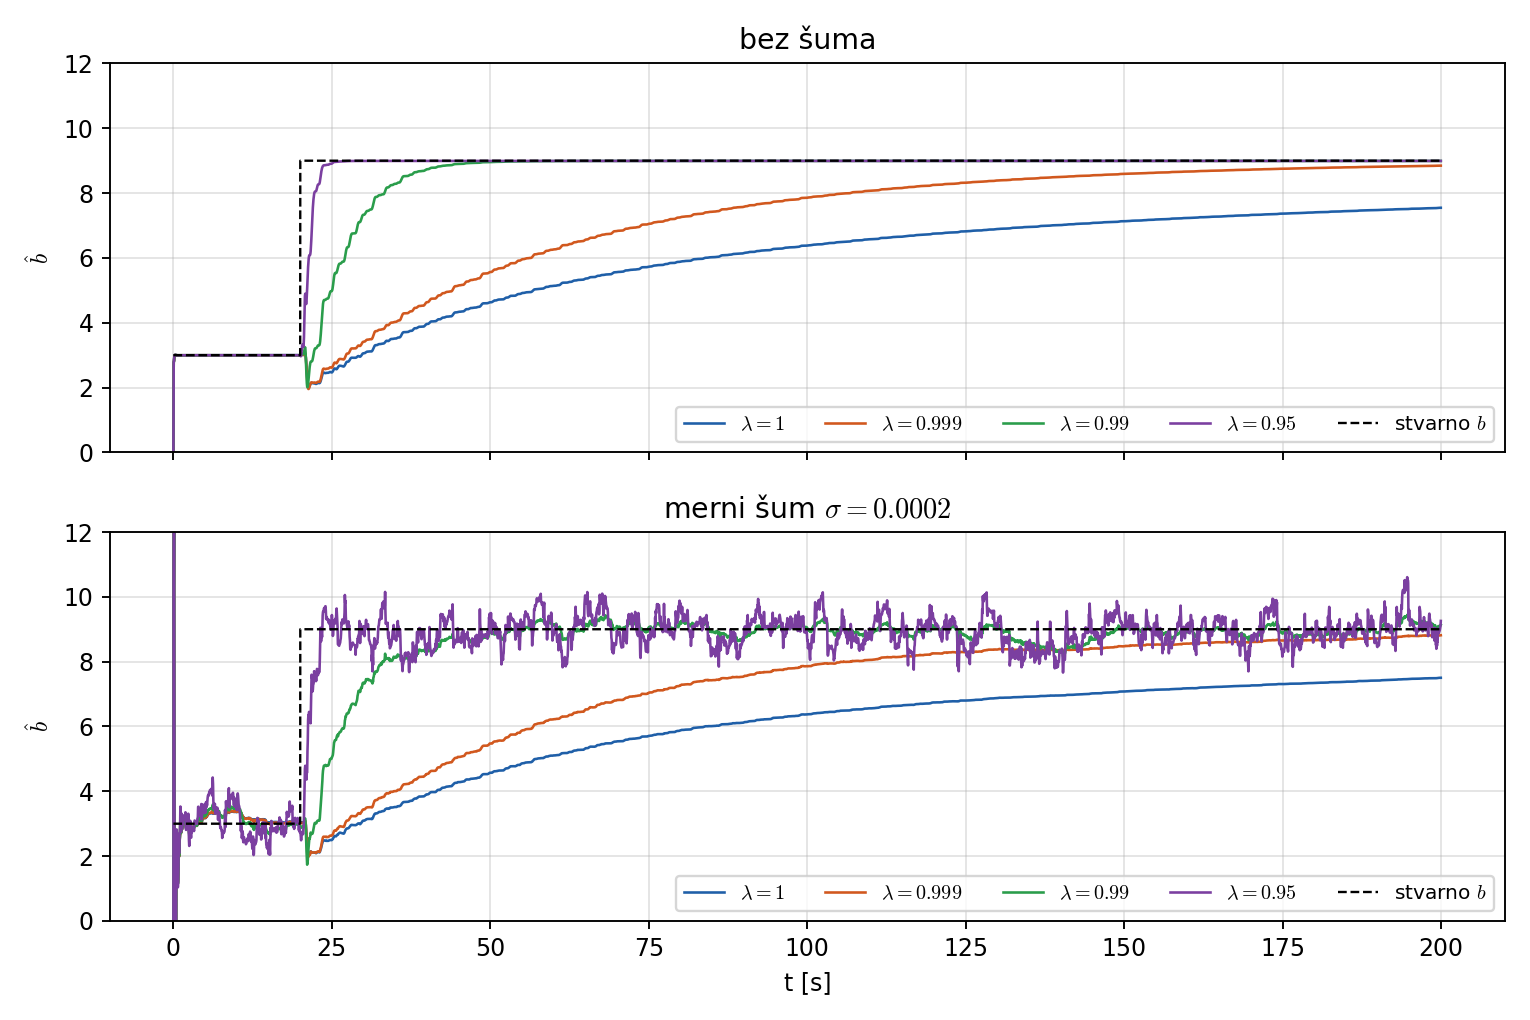
\includegraphics[width=0.9\linewidth,height=\textheight,keepaspectratio,alt={Procena b̂ posle promene b sa 3 na 9 u t = 20 s (Ts = 0,05 s). Gore bez šuma: λ = 1 ne stiže do 9 ni posle 180 s, a manje λ prati brže. Dole sa malim mernim šumom: λ = 0,95 je najbrži, ali procena najviše skače}]{figures/rls_lambda.png}
\caption{Procena b̂ posle promene b sa 3 na 9 u t = 20 s (Ts = 0,05 s). Gore bez šuma: λ = 1 ne stiže do 9 ni posle 180 s, a manje λ prati brže. Dole sa malim mernim šumom: λ = 0,95 je najbrži, ali procena najviše skače}
\end{figure}

\begin{longtable}[]{@{}lll@{}}
\caption{Kompromis pri izboru \(\lambda\)}\tabularnewline
\toprule\noalign{}
& Manje \(\lambda\) & Veće \(\lambda\) (bliže 1) \\
\midrule\noalign{}
\endfirsthead
\toprule\noalign{}
& Manje \(\lambda\) & Veće \(\lambda\) (bliže 1) \\
\midrule\noalign{}
\endhead
\bottomrule\noalign{}
\endlastfoot
praćenje promene & brzo & sporo \\
osetljivost na šum & velika, procena skače & mala, procena glatka \\
memorija \(T_s/(1-\lambda)\) & kratka & duga \\
\end{longtable}

Izbor \(\lambda\) ne ugrožava stabilnost samog estimatora, nego menja osetljivost (brzinu i šum): „ne znam da postoji \(\lambda\) za koju je algoritam nestabilan'' \izvor{snimak rekurzivni algoritam najmanjih kvadrata, 105. min}. Opasnost od premalog \(\lambda\) uz slabu pobudu je covariance windup (ispod).

U svesci je pitanje ostalo nedovršeno: „malo \(\lambda\) loše za šum; veliko \(\lambda\) loše zbog \_\_\_?''. Odgovor: veliko \(\lambda\) \textbf{sporo prati promene} parametara, pa adaptivni regulator dugo radi sa pogrešnim modelom.

\textbf{Covariance windup.} Kada signali nisu bogati (npr. konstantna referenca), \(\varphi\varphi^T\) ne donosi novu informaciju u nekim pravcima, a \(P\) se svakim korakom deli sa \(\lambda\). \(P\) tada eksponencijalno raste, i kada pobuda ponovo stigne, procena naglo skoči. Lekovi: dovoljno blizu 1 \(\lambda\), stalna pobuda ili ograničenje \(P\) (npr. reset \(P\) ili gornja granica traga). Referentno rešenje projekta resetuje \(P\) na početku svake faze identifikacije.

\textbf{Uslovno ažuriranje.} Na predavanju je predložena i jednostavna zaštita: ako je ulaz slab (npr. konstanta), \(\varphi\) je blizu nule i novo merenje ne nosi informaciju. Tada je i vektor pojačanja \(P\varphi\) mali. Umesto da se računa njegova norma, gleda se skalar \(\varphi^TP\varphi\): ako je manji od praga, ažuriranje se preskače i zadržavaju se stari \(\hat\theta\) i \(P\). Tako algoritam ne „zaboravlja'' dobra stara merenja zbog loših novih \izvor{P09 snimak, 44.--50. min}. Prag sa predavanja \izvor{P09 snimak, 50.--51. min}:

\[\varphi^TP\varphi < \varepsilon\,(1 - \lambda)\ \Rightarrow\ \text{ne ažurirati},\qquad \varepsilon \approx 0{,}5 \text{ do } 2 .\]

Obrazloženje (približno, za stacionaran režim sa pobudom): \(\varphi^TP\varphi\) se tada ustali oko veličine reda \(1 - \lambda\), pa vrednost ispod toga znači da novo merenje ne nosi informaciju.

\textbf{Robusne modifikacije: zasićenje i mrtva zona.} U zakonu za \(\hat\theta\) se umesto greške predikcije \(\tilde\eta\) može koristiti \(f(\tilde\eta)\) \izvor{P09 snimak, 54.--62. min}:

\begin{itemize}
\item \textbf{zasićenje} za velike greške (šum, slučajan skok merenja), npr. ograničenje sa \texttt{if} ili \(f = \frac{\tilde\eta}{1 + |\tilde\eta|}\) (vrednosti između \(-1\) i \(1\)), da jedno loše merenje ne pomeri procenu mnogo;
\item \textbf{mrtva zona} za vrlo male greške: kad je greška mala, sistem je ustaljen i ažuriranje se preskače, da šum ne „šeta'' procenu;
\item u normalnom opsegu \(f(\tilde\eta) = \tilde\eta\).
\end{itemize}

Predlog „uzimati samo 50--70 \% nove procene'' je na času odbijen: on usporava i razumne promene.

\textbf{RLS kao observer.} Parametri se ne menjaju, pa je „model'' za \(\theta\) sistem nultog reda: \(\theta(k+1) = \theta(k)\), sa „izlazom'' \(\eta = \varphi^T\theta\). Diskretni observer za takav sistem je \(\hat\theta(k+1) = \hat\theta(k) + L\big(\eta - \varphi^T\hat\theta(k)\big)\), što je tačno oblik RLS-a sa \(L = P\varphi\). Moglo bi se uzeti i konstantno \(L\), ali „matrica \(C\)„ je ovde \(\varphi^T\), koja se stalno menja, pa je teško naći konstantno pojačanje koje uvek daje stabilnu grešku. RLS to rešava tako što \(P\) računa u svakom koraku \izvor{P09 snimak, 37.--43. min}. Ista veza objašnjava zašto je RLS blizak Kalmanovom filtru.

\textbf{Šta pokazati u simulaciji.} Preporuka sa predavanja: u modelu napraviti opciju da se parametar procesa u jednom trenutku promeni (\emph{Clock} + \emph{Switch}), pa uporediti koliko brzo običan RLS i RLS sa \(\lambda\) „uhvate'' novu vrednost. \(\lambda\) je jedini dodatni ulazni parametar, a njegov uticaj se najbolje vidi tako što se menja i posmatra \izvor{P09 snimak, 35.--36. min}.

Domaći sa predavanja \izvor{P09 snimak, 97.--99. min}: (1) RLS iz prethodnog domaćeg dopuniti sa \(\lambda\) i uslovnim ažuriranjem; (2) skok parametra, poređenje \(\lambda = 1\) i \(\lambda < 1\); (3) dodati konstantan poremećaj na ulaz i pokazati da je procena pogrešna (pristrasna); (4) signale za identifikaciju filtrirati \textbf{propusnikom opsega} i pokazati da je procena ponovo tačna (poglavlje o projektu).

\subsection{Implementacija u Simulinku}

RLS je diskretan algoritam. U Simulinku se piše u \textbf{MATLAB Function} bloku, a memorija se čuva u \texttt{persistent} promenljivim. Blok se podesi da radi diskretno: desni klik, \emph{Explore} (Model Explorer), \emph{Update method: Discrete}, \emph{Sample time} \(T_s\).

\begin{verbatim}
function theta = rls(uf, yf, yf_dot, yf_2dot)
    lambda = 0.99;  alpha = 9999;
    persistent th P
    if isempty(th), th = zeros(3,1); P = alpha*eye(3); end
    eta = yf_2dot;
    phi = [-yf_dot; -yf; uf];                    % theta = [a1; a0; b]
    P  = (P - (P*(phi*phi')*P)/(lambda + phi'*P*phi))/lambda;
    th = th + P*phi*(eta - phi'*th);             % phi' (transponovano!)
    theta = th;
end
\end{verbatim}

Ulazi su filtrirani signali iz poglavlja o MNK (kontinualni proces), ili zakašnjeni odbirci \(y(k-1)\), \(y(k-2)\), \(u(k-1)\), \(u(k-2)\) (diskretni ARX model, varijanta B projekta). Česta greška (i u nekim prepisima sa table): \texttt{eta\ -\ phi*theta\_\allowbreak{}p}, a mora biti \texttt{phi\textquotesingle{}}. Redosled je bitan: prvo se računa novo \(P_{t+1}\), pa se ono koristi u zakonu za \(\hat\theta\).

Kako se ulazi dobijaju u Simulinku:

\begin{itemize}
\item \textbf{Kontinualni model:} filtri su kontinualni blokovi \emph{Transfer Fcn} (poglavlje o MNK), a diskretni MATLAB Function blok ih sam „uzorkuje'' na svakih \(T_s\). Ovde \(T_s\) treba da bude bar nekoliko puta manje od \(T_f\) (u primeru sa časa \(T_f = 0{,}01\), u jednom rešenju domaćeg \(T_f = 0{,}05\) uz \(T_s = 0{,}01\)).
\item \textbf{Diskretni ARX:} \(y\) i \(u\) prolaze kroz lanac blokova \emph{Unit Delay} sa istim \(T_s\); \(\eta = y(k)\), \(\varphi = [-y(k-1);\ -y(k-2);\ u(k-1);\ u(k-2)]\). Pošto \(\varphi\) sadrži samo prošle odbirke, nema algebarske petlje.
\item U \(\varphi\) ide \(u\) koje \textbf{stvarno ulazi u proces} (posle oduzimanja \(\hat d\), posle zasićenja ako postoji), inače estimator uči pogrešan odnos \(u \to y\).
\end{itemize}

\textbf{Kako proveriti da RLS radi.} Prvo ga testiraj u otvorenoj sprezi, na procesu sa poznatim parametrima i bogatim ulazom (npr. 3 sinusoide za 3 parametra, kao na času). Grafici:

\begin{enumerate}
\def\labelenumi{\arabic{enumi}.}
\item \(\hat\theta(t)\) i tačne vrednosti isprekidano: posle nekoliko sekundi procena treba da legne na tačnu (bez šuma do na 3 decimale), a posle promene procesa da stigne novu za vreme reda \(T_{mem}\);
\item greška predikcije \(\eta - \varphi^T\hat\theta\) (pre ažuriranja): posle početka treba da padne na nivo šuma;
\item \texttt{trace(P)}: posle početnog pada treba da ostane ograničen. Ako eksponencijalno raste, to je covariance windup (nema pobude).
\end{enumerate}

Ako procena ne ide na tačne vrednosti, a greška predikcije je mala, problem je pobuda (proveri broj sinusoida); ako je i greška predikcije velika, problem je u \(\eta\) i \(\varphi\) (znak, kašnjenje, filter).

\begin{ispit}
Izvođenje RLS-a \textbf{se ne traži napamet}: na predavanju je rečeno „ne očekuje se da znate ovako nešto na pamet \ldots{} možete koristiti svu literaturu'' \izvor{P08 snimak, 112.--113. min}, a i sama predavačica formulu „ne zna napamet, zna da izvede'' \izvor{P09 snimak, 2.--3. min}. Treba umeti objasniti tri koraka (rekurzija za \(P^{-1}\), zakon za \(\hat\theta\), lema o inverziji), šta su \(P\), \(\varphi\), \(\eta\), i objasniti \(\lambda\): modifikovan kriterijum sa \(\lambda^{t-k}\), formula za \(P\), memorija \(1/(1-\lambda)\), kompromis brzina/šum. Zamke: \(P_0\) mora biti veliko, imenilac \(\lambda + \varphi^TP\varphi\) je skalar, i bez pobude nema učenja (covariance windup).
\end{ispit}

\section{Stabilnost po Ljapunovu i gradijentni algoritam}

\subsection{Ideja}

Gradijentni algoritam menja procenu \(\hat\theta\) u smeru u kome kvadrat trenutne greške najbrže opada. Zakon adaptacije je diferencijalna jednačina, dakle dinamički sistem. Da je taj sistem „dobar'', tj. da greška zaista nestaje, ne dokazujemo simulacijom nego \textbf{Ljapunovljevom funkcijom}. Obrnuto se isto koristi za projektovanje: izabere se \(V\), pa se zakon adaptacije izabere tako da je \(\dot V \le 0\).

\subsection{Stabilnost po Ljapunovu (koliko treba za ovaj deo)}

Kratak podsetnik; pun pregled (LaSalle, globalna stabilnost, indirektna metoda) je u beleškama za Nelinearno upravljanje, poglavlje „Ljapunovljeva stabilnost''. Za \(\dot x = f(x)\) sa ravnotežom \(x_0\):

\begin{itemize}
\item \textbf{stabilnost:} za svako \(\varepsilon > 0\) postoji \(\delta > 0\) tako da iz \(\|x(0) - x_0\| < \delta\) sledi \(\|x(t) - x_0\| < \varepsilon\) za \textbf{svako} \(t \ge 0\) (ostaje blizu, ne mora da stigne u \(x_0\));
\item \textbf{asimptotska:} stabilnost i još \(x(t) \to x_0\); \textbf{eksponencijalna:} \(\|x(t) - x_0\| \le M\|x(0) - x_0\|e^{-\lambda t}\) (stabilni linearni sistemi su uvek takvi).
\end{itemize}

Hijerarhija: eksponencijalna \(\Rightarrow\) asimptotska \(\Rightarrow\) stabilnost. Asimptotska dozvoljava da stanje osciluje pre nego što stigne u ravnotežu, a eksponencijalna traži da odstupanje bude ograničeno opadajućom eksponencijalom \izvor{snimak stabilnost i gradijentni algoritam 1, 10.--14. min}.

Na predavanju i u svesci su uloge \(\varepsilon\) i \(\delta\) zamenjene („ako je \(\|x_0 - x_r\| < \varepsilon\), sledi \(\|x(t) - x_r\| < \delta\)„) \izvor{snimak stabilnost i gradijentni algoritam 1, 4.--8. min}. Ispravno je kako stoji gore: za \textbf{svako} \(\varepsilon\) (dozvoljeno odstupanje, zadaje se prvo) postoji \(\delta\) (dovoljno blizak početak). U obrnutom redosledu („za svaki početni \(\varepsilon\) postoji neko \(\delta\)„) definicija bi tvrdila samo da putanja ostaje \textbf{ograničena}, ne i da ostaje proizvoljno blizu ravnoteže.

\textbf{Teorema Ljapunova.} Ako je \(V(x_0) = 0\), \(V(x) > 0\) za \(x \ne x_0\) i

\[\dot V = \frac{\partial V}{\partial x}f(x) \le 0\ \Rightarrow\ \text{stabilna},\qquad \dot V < 0\ (x \ne x_0)\ \Rightarrow\ \text{asimptotski stabilna}.\]

\(V\) je uopštena energija. Uslov je \textbf{dovoljan, ne i potreban}. Primer: za \(\dot x_1 = -x_1^3 + 2x_2^3\), \(\dot x_2 = -2x_1x_2^2\) i \(V = \frac12(x_1^2 + x_2^2)\) je \(\dot V = -x_1^4 + 2x_1x_2^3 - 2x_1x_2^3 = -x_1^4 \le 0\): stabilna, a ovaj \(V\) ne dokazuje asimptotsku (\(\dot V = 0\) na osi \(x_1 = 0\)).

Kako birati \(V\): nema tačnog pravila; u \(V\) se stavlja \textbf{ono što želimo da iščezne}, najčešće kao zbir kvadrata (ako ravnoteža nije u nuli, pomeri se: \(x - x_r\)). Ako za izabrano \(V\) uslov ne prođe, to \textbf{ne dokazuje nestabilnost}, nego samo da kandidat nije dobar \izvor{snimak stabilnost i gradijentni algoritam 1, 20.--28. min}. Kod adaptacije treba da iščezne greška procene, pa je \(V\) funkcija od \(\tilde\theta\).

\subsection{Gradijentni algoritam: jedan parametar (MIT pravilo)}

\textbf{Postavka.} Proces \(y = \theta u\) i model sa procenom \(\hat y = \hat\theta u\). Greška izlaza je \(\tilde y = y - \hat y\).

\begin{figure}
\centering
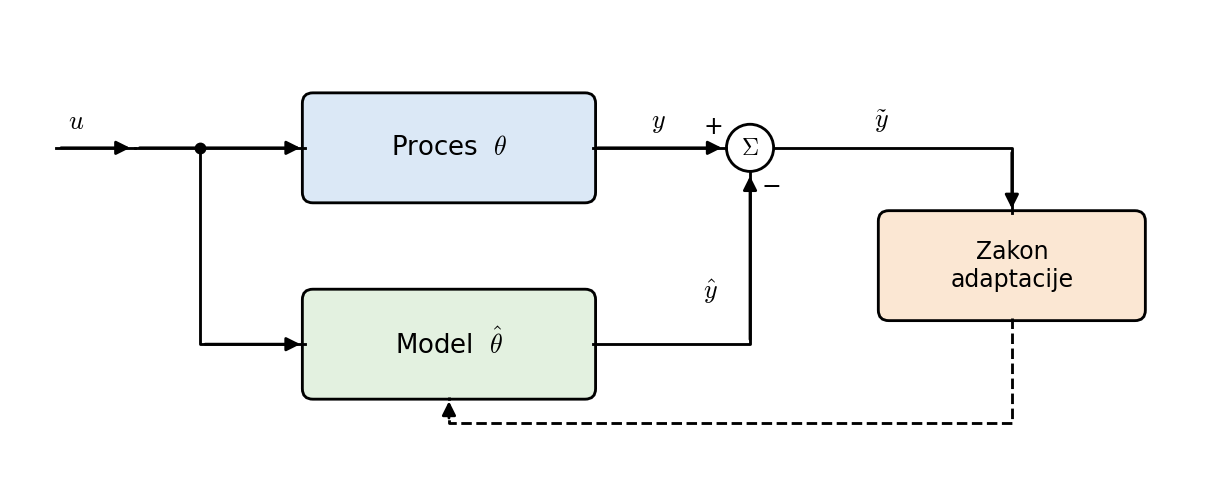
\includegraphics[width=0.75\linewidth,height=\textheight,keepaspectratio,alt={Opšta šema estimacije: isti ulaz ide na proces i na model sa procenjenim parametrima, a greška izlaza pokreće zakon adaptacije}]{figures/blok_model_proces.png}
\caption{Opšta šema estimacije: isti ulaz ide na proces i na model sa procenjenim parametrima, a greška izlaza pokreće zakon adaptacije}
\end{figure}

\textbf{Izvođenje.} Kriterijum je trenutni kvadrat greške, \(J = \frac12\tilde y^2\). Parametar se menja \textbf{suprotno od gradijenta} (MIT pravilo):

\[\dot{\hat\theta} = -\gamma\frac{\partial J}{\partial\hat\theta} = -\gamma\,\tilde y\,\frac{\partial\tilde y}{\partial\hat\theta} = -\gamma\,\tilde y\,(-u)\qquad\Rightarrow\qquad \dot{\hat\theta} = \gamma\,u\,\tilde y .\]

\(\gamma > 0\) je korak (brzina učenja). U Simulinku je to lanac blokova \izvor{snimak stabilnost i gradijentni algoritam 2, 0.--3. min}: \(\tilde y\) se pomnoži sa \(u\) (\emph{Product}) i sa \(\gamma\) (\emph{Gain}), prođe kroz \emph{Integrator} i daje \(\hat\theta\), a \(\hat\theta\) pomnoženo sa \(u\) je izlaz modela \(\hat y\).

\textbf{Dokaz konvergencije.} Želimo da iščezne \(\tilde\theta = \theta - \hat\theta\). \(\theta\) je konstanta, pa je \(\dot{\tilde\theta} = -\dot{\hat\theta}\). Kandidat (sa \(\gamma\) unapred, da bi se skratilo):

\[V = \frac{1}{2\gamma}\tilde\theta^2,\qquad \dot V = \frac1\gamma\tilde\theta\dot{\tilde\theta} = -\frac1\gamma\tilde\theta\,\gamma u\tilde y = -(u\tilde\theta)\tilde y = -\tilde y^2 \le 0,\]

jer je \(\tilde y = \theta u - \hat\theta u = u\tilde\theta\).

\begin{kljucna}
\(\dot V = -\tilde y^2 \le 0\), a ne \(< 0\) (u svesci piše \(< 0\)). \(\dot V = 0\) kad je \(\tilde y = 0\), a to se dešava i kad je \(u = 0\), iako je \(\tilde\theta \ne 0\). Garantovano je da greška \textbf{izlaza} ide ka nuli. Da bi i \textbf{parametar} konvergirao, ulaz mora stalno da pobuđuje sistem (persistent excitation).
\end{kljucna}

\textbf{Uticaj \(\gamma\).} Veće \(\gamma\) daje bržu konvergenciju. U diskretnoj implementaciji (Ojler, korak \(h\)), \(\hat\theta_{k+1} = \hat\theta_k + h\gamma u\tilde y\), pa je greška \(\tilde\theta_{k+1} = (1 - h\gamma u^2)\tilde\theta_k\). Za \(h\gamma u^2 > 2\) faktor je po modulu veći od 1 i algoritam divergira („preskače'' minimum). Manje \(\gamma\) je sporije, ali sigurnije. Na snimku je dodatno objašnjeno da je fiksni korak loš na oba kraja: gde je kriterijum strm, gradijent je veliki i procena skače (može da preskoči minimum i ide „cik-cak''), a blizu minimuma kriterijum je ravan, gradijent mali i konvergencija spora. Zato postoje varijante sa promenljivim (adaptivnim) korakom \izvor{P08 snimak, 41.--45. min}. Van Simulinka (npr. kod u MATLAB-u ili C-u) zakon se \textbf{mora} pisati diskretno, Ojlerom unapred: \(\hat\theta_{novo} = \hat\theta_{staro} + T\gamma\tilde yu\); to je sam parametar, a ne njegov priraštaj \izvor{P08 snimak, 56.--59. min}.

\begin{figure}
\centering
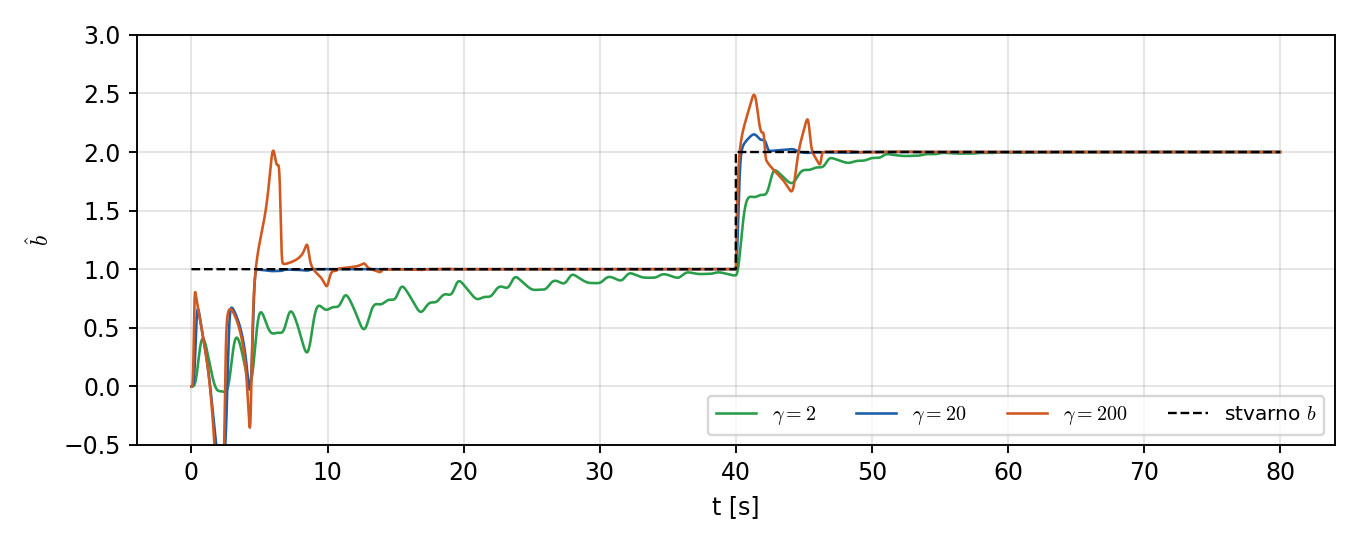
\includegraphics[width=0.8\linewidth,height=\textheight,keepaspectratio,alt={Uticaj koraka γ na procenu b̂ (proces b/(s+a), b skače sa 1 na 2 u t = 40 s). γ = 2 sporo konvergira, γ = 20 brzo i mirno, a γ = 200 preskače i osciluje posle svake promene}]{figures/gradijent_gama.png}
\caption{Uticaj koraka γ na procenu b̂ (proces b/(s+a), b skače sa 1 na 2 u t = 40 s). γ = 2 sporo konvergira, γ = 20 brzo i mirno, a γ = 200 preskače i osciluje posle svake promene}
\end{figure}

\subsection{Više parametara}

\textbf{Postavka:} \(\eta = \varphi^T\theta\), \(\hat\eta = \varphi^T\hat\theta\), \(\tilde\eta = \eta - \hat\eta = \varphi^T\tilde\theta\) (skalar, jedno merenje u trenutku).

\textbf{Izvođenje.} \(J = \frac12\tilde\eta^2\), a \(\frac{\partial\tilde\eta}{\partial\hat\theta} = -\varphi\):

\[\dot{\hat\theta} = -\Gamma\frac{\partial J}{\partial\hat\theta} = -\Gamma\,(-\varphi)\,\tilde\eta\qquad\Rightarrow\qquad \dot{\hat\theta} = \Gamma\,\varphi\,\tilde\eta .\]

\(\Gamma\) je pozitivno definitna \(n\times n\) matrica, obično dijagonalna, pa svaki parametar ima svoj korak (npr. \(\Gamma = \operatorname{diag}(1, 4, 5)\); skalar \(\gamma = 3\) je isto što i \(\Gamma = 3I\)) \izvor{snimak stabilnost i gradijentni algoritam 2, 7.--9. min}. To je korisno kad su parametri različitog reda veličine. Dimenzije: \((n\times n)(n\times 1)(1\times 1)\). U nekim prepisima uz \(\tilde\eta\) stoji \(n\times 1\), a tačno je \(1\times 1\).

\textbf{Konvergencija.} \(V = \frac12\tilde\theta^T\Gamma^{-1}\tilde\theta\):

\[\dot V = \tilde\theta^T\Gamma^{-1}\dot{\tilde\theta} = -\tilde\theta^T\Gamma^{-1}\Gamma\varphi\tilde\eta = -(\tilde\theta^T\varphi)\tilde\eta = -\tilde\eta^2 \le 0 .\]

\subsection{Ljapunovljev pristup projektovanju zakona adaptacije}

Isti račun može da se okrene. Umesto da prvo izaberemo gradijent pa proverimo stabilnost, izaberemo \(V = \frac12\tilde\theta^T\Gamma^{-1}\tilde\theta\) i tražimo zakon \(\dot{\hat\theta}\) takav da je \(\dot V \le 0\):

\[\dot V = -\tilde\theta^T\Gamma^{-1}\dot{\hat\theta} .\]

Izbor \(\dot{\hat\theta} = \Gamma\varphi\tilde\eta\) daje \(\dot V = -\tilde\theta^T\varphi\,\varphi^T\tilde\theta = -\tilde\eta^2\). Za ovaj problem Ljapunovljev dizajn i MIT pravilo daju \textbf{isti} zakon. Razlika je što Ljapunovljev pristup garantuje stabilnost po konstrukciji, dok MIT pravilo u opštem slučaju (npr. kod direktnog MRAC-a) može da bude nestabilno za veliko \(\gamma\).

\subsection{Uslov dovoljne pobude (persistent excitation)}

Iz \(\tilde\eta = \varphi^T\tilde\theta \to 0\) sledi \(\tilde\theta \to 0\) samo ako \(\varphi\) „obilazi'' sve pravce u prostoru parametara. Formalno, \(\varphi\) je \textbf{dovoljno pobudan} ako postoje \(T > 0\) i \(\alpha > 0\) tako da je za svako \(t\)

\[\int_t^{t+T}\varphi(\tau)\varphi^T(\tau)\,d\tau \ \ge\ \alpha I .\]

To je vremenski kontinualna verzija uslova da je \(\Phi\) punog ranga kod MNK. Praktično (pravilo kursa, poglavlje o MNK): ulaz mora imati bar \(n\) različitih učestanosti za \(n\) parametara; teorijski minimum je \(\lceil n/2\rceil\). Sa jednom sinusoidom i tri parametra \(\tilde\eta \to 0\), ali parametri ne idu na tačne vrednosti.

\subsection{Problem: sve zavisi od trenutnih vrednosti}

Običan gradijent koristi samo trenutne \(\varphi\) i \(\tilde\eta\). Brzo reaguje na promenu parametra, ali je \textbf{jako osetljiv na šum}: svaki skok u signalu shvati kao promenu parametra. Ostale mane sa predavanja \izvor{P08 snimak, 62.--64. min}: fiksan korak (spor gde je nagib mali) i osetljivost na \textbf{izbor početne procene}. Kod MNK na procenu utiču sva prethodna merenja. Zato se uvodi uticaj prošlosti, slično I dejstvu kod PID-a.

\subsection{Gradijentni algoritam sa integralnim kriterijumom}

\textbf{Postavka.} Kriterijum je integral kvadrata grešaka sa eksponencijalno opadajućom težinom:

\[J(\hat\theta) = \frac12\int_0^te^{-\beta(t-\tau)}\,\tilde\eta^2(\tau, t)\,d\tau,\qquad \tilde\eta(\tau, t) = \eta(\tau) - \varphi^T(\tau)\hat\theta(t),\qquad \beta > 0 .\]

\(\tilde\eta(\tau, t)\) je greška koju bi \textbf{današnja} procena napravila na \textbf{starom} merenju iz trenutka \(\tau\). Blizu \(\tau = t\) težina je 1, a starija merenja imaju sve manju težinu. (U prepisu sveske stoji \(\varphi(t)\), a mora biti \(\varphi(\tau)\).)

\textbf{Izvođenje gradijenta.} \(\hat\theta(t)\) ne zavisi od \(\tau\), pa izlazi ispred integrala:

\[\frac{\partial J}{\partial\hat\theta} = -\int_0^te^{-\beta(t-\tau)}\varphi(\tau)\big[\eta(\tau) - \varphi^T(\tau)\hat\theta(t)\big]d\tau = R(t)\,\hat\theta(t) - Q(t),\]

\[R(t) = \int_0^te^{-\beta(t-\tau)}\varphi(\tau)\varphi^T(\tau)\,d\tau,\qquad Q(t) = \int_0^te^{-\beta(t-\tau)}\varphi(\tau)\eta(\tau)\,d\tau .\]

Zakon adaptacije:

\[\dot{\hat\theta} = -\Gamma\big[R(t)\hat\theta - Q(t)\big]\]

\textbf{Kako računati \(R\) i \(Q\) bez čuvanja istorije.} Rešenje sistema \(\dot x = -\beta x + v\) sa \(x(0) = 0\) je \(x(t) = \int_0^te^{-\beta(t-\tau)}v(\tau)\,d\tau\). To je upravo oblik \(R\) i \(Q\), pa:

\[\dot R = -\beta R + \varphi\varphi^T,\quad R(0) = 0,\qquad \dot Q = -\beta Q + \varphi\,\eta,\quad Q(0) = 0 .\]

\(R\) i \(Q\) su izlazi niskopropusnih filtara prvog reda. (U prepisu stoji \(\dot Q = -\beta Q + \eta\), bez \(\varphi\); dimenzije pokazuju da mora \(\varphi\eta\).)

\textbf{Stabilnost.} Bez šuma je \(\eta = \varphi^T\theta\), pa je \(Q = R\theta\) i

\[\dot{\hat\theta} = -\Gamma R(\hat\theta - \theta) = \Gamma R\tilde\theta,\qquad V = \tfrac12\tilde\theta^T\Gamma^{-1}\tilde\theta,\qquad \dot V = -\tilde\theta^TR\,\tilde\theta \le 0,\]

jer je \(R\) zbir (integral) matrica \(\varphi\varphi^T \ge 0\), dakle pozitivno semidefinitna. Uz dovoljnu pobudu \(R\) je pozitivno definitna i \(\tilde\theta \to 0\) eksponencijalno.

\begin{figure}
\centering
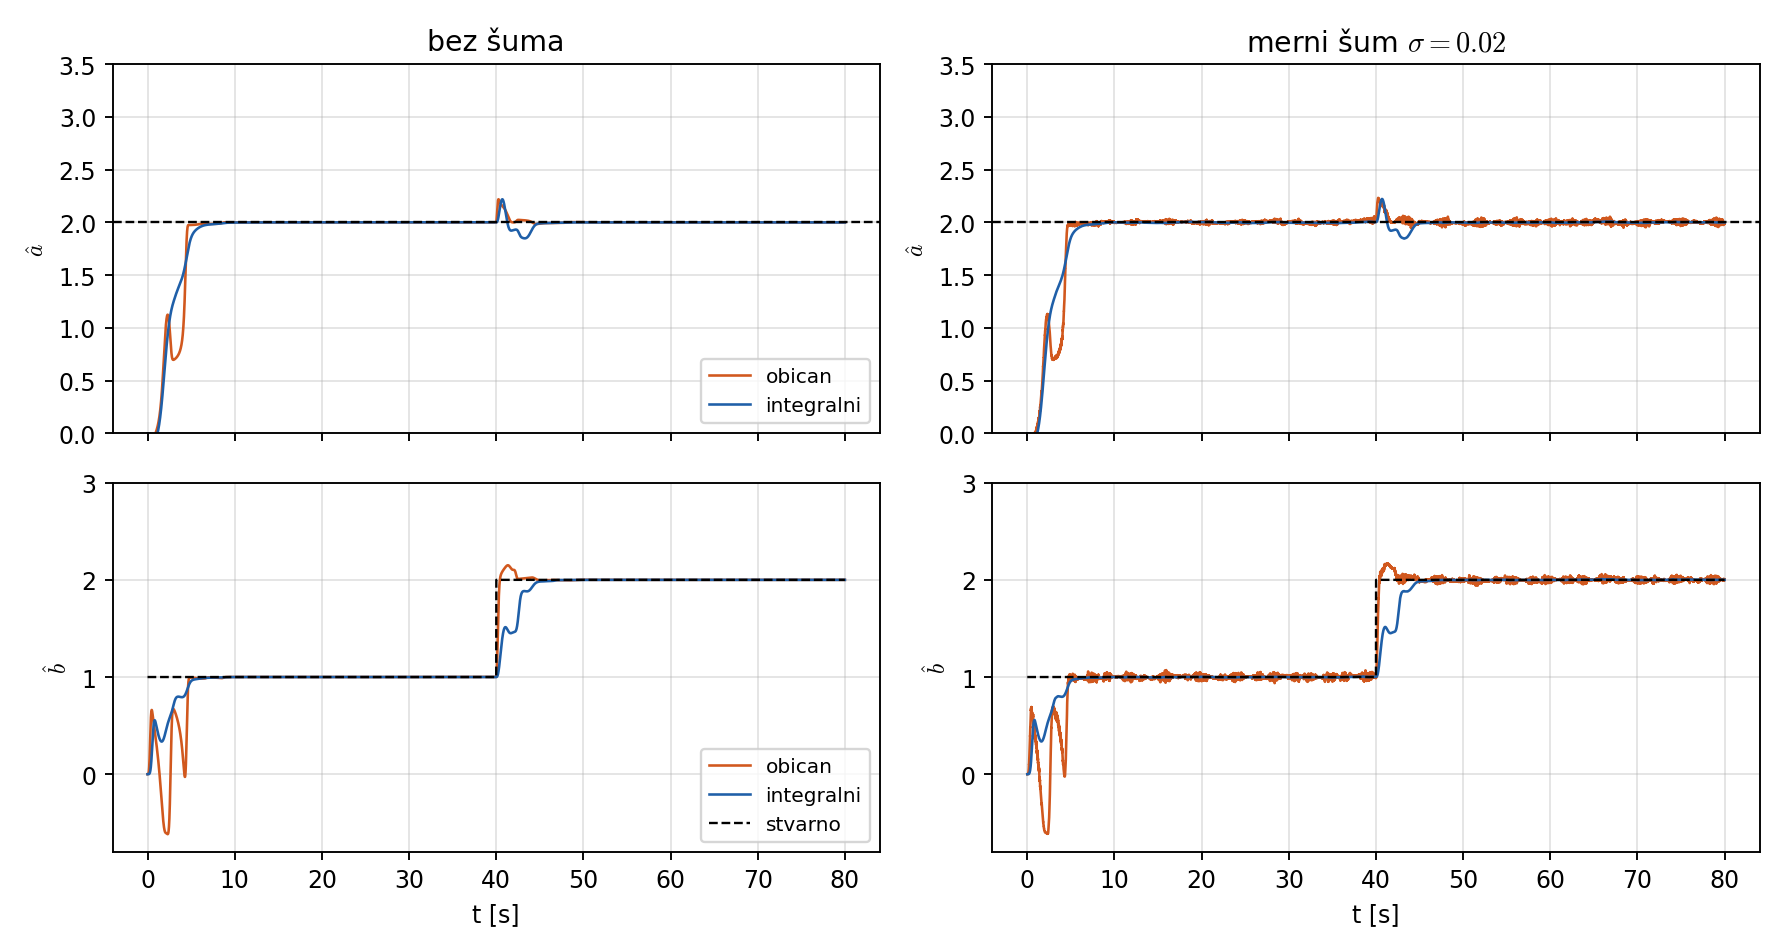
\includegraphics[width=0.95\linewidth,height=\textheight,keepaspectratio,alt={Poređenje običnog i integralnog gradijenta (Γ = 20I, β = 1), proces b/(s+a), b skače sa 1 na 2 u t = 40 s. Običan brže reaguje na promenu, ali ima cik-cak prelaz na početku i jače prenosi šum. Integralni ima glatku putanju i skoro ne vidi šum}]{figures/gradijent_poredjenje.png}
\caption{Poređenje običnog i integralnog gradijenta (Γ = 20I, β = 1), proces b/(s+a), b skače sa 1 na 2 u t = 40 s. Običan brže reaguje na promenu, ali ima cik-cak prelaz na početku i jače prenosi šum. Integralni ima glatku putanju i skoro ne vidi šum}
\end{figure}

\begin{longtable}[]{@{}
  >{\raggedright\arraybackslash}p{(\linewidth - 6\tabcolsep) * \real{0.1716}}
  >{\raggedright\arraybackslash}p{(\linewidth - 6\tabcolsep) * \real{0.1865}}
  >{\raggedright\arraybackslash}p{(\linewidth - 6\tabcolsep) * \real{0.3162}}
  >{\raggedright\arraybackslash}p{(\linewidth - 6\tabcolsep) * \real{0.3257}}@{}}
\caption{Poređenje algoritama za estimaciju (rezultati sa slike: std(\(\hat b\)) sa šumom 0,014 za običan i 0,002 za integralni)}\tabularnewline
\toprule\noalign{}
\begin{minipage}[b]{\linewidth}\raggedright
\end{minipage} & \begin{minipage}[b]{\linewidth}\raggedright
Običan gradijent
\end{minipage} & \begin{minipage}[b]{\linewidth}\raggedright
Integralni gradijent
\end{minipage} & \begin{minipage}[b]{\linewidth}\raggedright
RLS sa \(\lambda\)
\end{minipage} \\
\midrule\noalign{}
\endfirsthead
\toprule\noalign{}
\begin{minipage}[b]{\linewidth}\raggedright
\end{minipage} & \begin{minipage}[b]{\linewidth}\raggedright
Običan gradijent
\end{minipage} & \begin{minipage}[b]{\linewidth}\raggedright
Integralni gradijent
\end{minipage} & \begin{minipage}[b]{\linewidth}\raggedright
RLS sa \(\lambda\)
\end{minipage} \\
\midrule\noalign{}
\endhead
\bottomrule\noalign{}
\endlastfoot
kriterijum & trenutni \(\tilde\eta^2\) & \(\int e^{-\beta(t-\tau)}\tilde\eta^2\) & \(\sum\lambda^{t-k}\tilde\eta_k^2\) \\
pojačanje & konstantno \(\Gamma\) & \(\Gamma R\) & adaptivno \(P\varphi\) \\
reakcija na promenu & najbrža & sporija & zavisi od \(\lambda\) \\
osetljivost na šum & velika & mala & zavisi od \(\lambda\) \\
memorija & nema & oko \(1/\beta\) s & oko \(T_s/(1-\lambda)\) \\
\end{longtable}

Integralni gradijent je blizak RLS-u sa zaboravljanjem: \(R \leftrightarrow P^{-1}\), \(\beta \leftrightarrow 1 - \lambda\).

\textbf{Implementacija u Simulinku.} Običan: MATLAB Function računa \(\Gamma\varphi(\eta - \varphi^T\hat\theta)\), a blok \emph{Integrator} daje \(\hat\theta\) (gotova rešenja: mapa domaćih). Integralni: dodatni integratori za \(R\) (\(n\times n\)) i \(Q\) (\(n\times 1\)), sa povratnom spregom \(-\beta\). Jednostavnije je sve napisati diskretno u jednom MATLAB Function bloku sa \texttt{persistent} promenljivim (Ojler, korak \(T_s\)):

\[R \leftarrow R + T_s(-\beta R + \varphi\varphi^T),\qquad Q \leftarrow Q + T_s(-\beta Q + \varphi\eta),\qquad \hat\theta \leftarrow \hat\theta - T_s\Gamma(R\hat\theta - Q).\]

\textbf{Kako izabrati \(\Gamma\) i \(\beta\).} Iz diskretne analize iznad: za običan gradijent mora biti \(T_s\gamma\,\varphi^T\varphi < 2\), pa se \(\gamma\) bira prema tipičnoj veličini \(\|\varphi\|^2\). Na primer, za \(\|\varphi\|^2 \approx 1\) i \(T_s = 10\) ms granica je \(\gamma < 200\), a razumno je \(\gamma \approx 10\) do \(50\), sa rezervom (slika sa tri \(\gamma\) gore pokazuje oba kraja). Ako signali jako menjaju veličinu, koristi se normalizovan korak \(\dot{\hat\theta} = \Gamma\varphi\tilde\eta/(1 + \varphi^T\varphi)\), kod kog je granica ista za svaku amplitudu (standardna praksa, nije rečeno na predavanju; tamo je samo rečeno da korak može biti promenljiv i da postoji „milion modifikacija''). Za integralni važi isto sa \(\lambda_{max}(\Gamma R)\) umesto \(\gamma\varphi^T\varphi\). \(\beta\) određuje memoriju od oko \(1/\beta\) sekundi: \(\beta = 1\) pamti oko 1 s.

Provera je ista kao kod RLS-a: \(\hat\theta(t)\) naspram tačnih vrednosti, greška \(\tilde\eta\) i reakcija na promenu parametra.

\begin{ispit}
Izvesti MIT pravilo \(\dot{\hat\theta} = \Gamma\varphi\tilde\eta\) i dokaz \(\dot V = -\tilde\eta^2 \le 0\) (znati zašto \(\le\), a ne \(<\), i šta je persistent excitation). Za integralni algoritam: kriterijum sa \(e^{-\beta(t-\tau)}\), gradijent \(R\hat\theta - Q\) i trik da su \(R\) i \(Q\) izlazi filtara. Uporediti sa RLS: \(\beta\) igra ulogu \(1-\lambda\).

Domaći sa predavanja \izvor{P08 snimak, 59.--62. min}: u Simulinku (kontinualno, sa integratorima) proceniti \(\theta\) za \(y = 3u\), pa dva parametra procesa prvog reda. U ranijoj generaciji: poređenje običnog i integralnog gradijenta na primeru sa dva parametra \izvor{snimak stabilnost i gradijentni algoritam 2, 37.--38. min}.
\end{ispit}

\section{Indirektno adaptivno upravljanje: završni projekat}

\subsection{Zadatak}

Individualno implementirati šemu \textbf{indirektnog adaptivnog upravljanja} koja radi u realnom vremenu. Estimacija parametara je \textbf{po izboru RLS ili gradijentni algoritam}, a projekat se brani \izvor{snimak rekurzivni algoritam najmanjih kvadrata, 112.--114. min}. Iz procena se formiraju matrice modela, u svakom trenutku se preračunavaju pojačanja regulatora po stanjima i observera, a \(k_r\) obezbeđuje jedinično statičko pojačanje. Treba pokazati šta se dešava kada se parametri procesa promene tokom simulacije.

\textbf{Recept sa predavanja} \izvor{P09 snimak, 87.--101. min}, „sklopiti sve što smo radili od početka u jednom projektu'':

\begin{enumerate}
\def\labelenumi{\arabic{enumi}.}
\item iz merenja \(u\), \(y\) proceniti parametre (proces drugog reda iz domaćeg);
\item od procena formirati \(\hat A\), \(\hat B\), \(\hat C\);
\item \textbf{dva poziva \texttt{acker}}: jedan za \(K\), drugi za pojačanje observera \(L\);
\item \textbf{observer stanja i poremećaja} (prošireni observer iz poglavlja o poremećajima) daje \(\hat x\) i \(\hat d\);
\item zakon upravljanja
  \[u = -K\hat x - \hat d + k_r r .\]
\end{enumerate}

Zahtevi za implementaciju \izvor{P09 snimak, 94.--97. i 104. min}:

\begin{itemize}
\item \textbf{minimum:} Simulink, može kontinualno, sklopljen od blokova sa domaćih;
\item \textbf{„top'' varijanta:} cela petlja (estimacija, projektovanje, observer, zakon upravljanja) kao \textbf{jedna diskretna MATLAB funkcija} koja na ulazu dobija \(r\) i \(y\), a na izlazu daje \(u\), jer se tako kod piše i na pravom kontroleru (u C-u);
\item predavačica pominje „template'' MATLAB funkcije iz prethodnih godina, sa spiskom šta funkcija treba da ima: vredi ga tražiti kod predmetnog nastavnika.
\end{itemize}

\textbf{Sklapati korak po korak}, „nemojte odjednom sve da sklapate pa ne znate gde vam je greška'' \izvor{P09 snimak, 96.--97. min}: (1) regulator po stanjima sa poznatim modelom; (2) dodati observer stanja i poremećaja; (3) tek onda u observer i regulator umesto fiksnih \(A\), \(B\), \(C\) dovesti procenjene matrice.

U ranijoj generaciji (audio snimak prof. Radović) šema je imala samo observer stanja i \(u = -K\hat x + k_rr\), bez \(\hat d\) \izvor{snimak rekurzivni algoritam najmanjih kvadrata, 108.--112. min}; P09 traži i estimator poremećaja, pa ga ove beleške uzimaju kao deo zadatka.

\begin{figure}
\centering
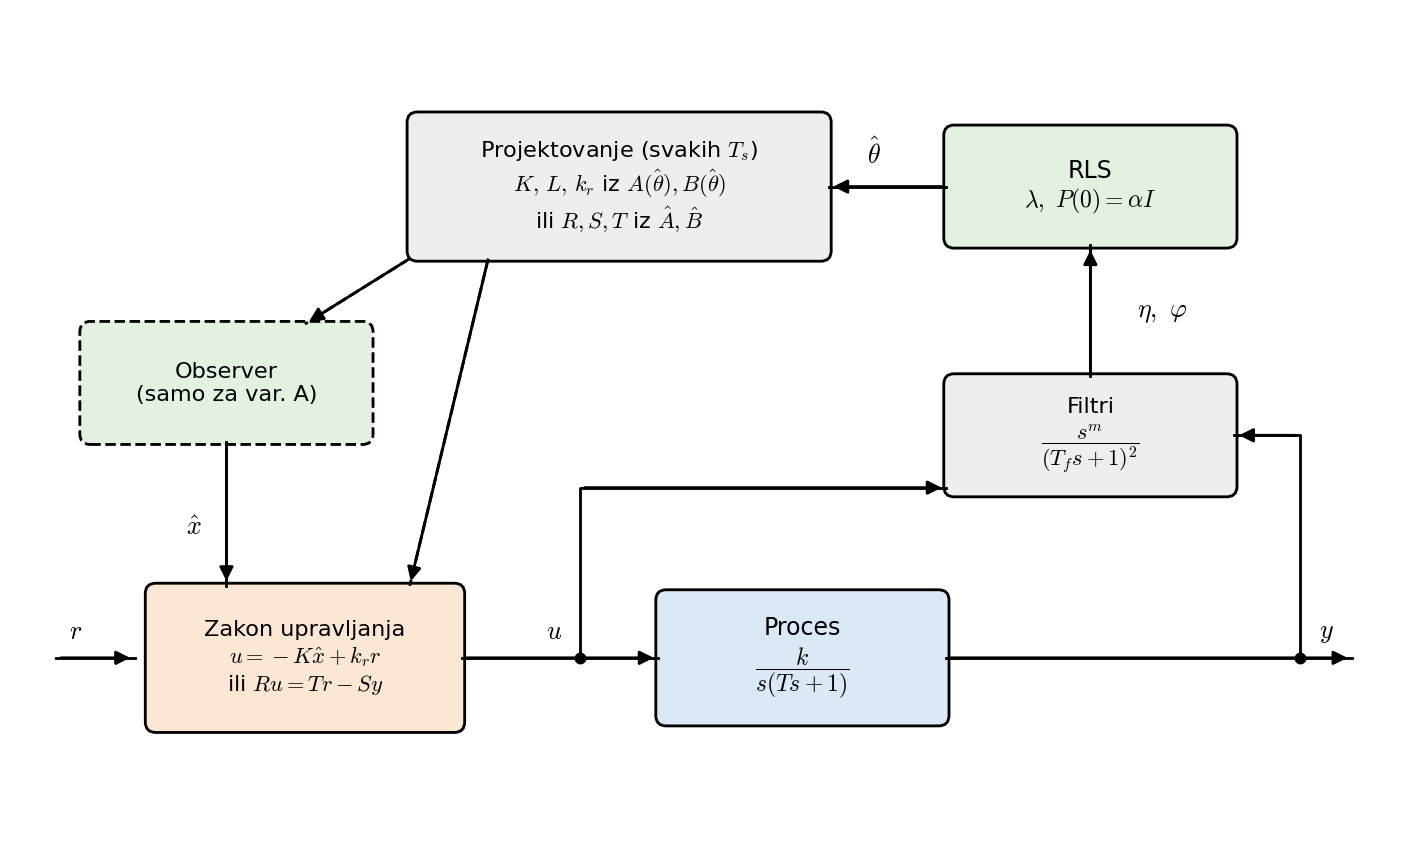
\includegraphics[width=0.9\linewidth,height=\textheight,keepaspectratio,alt={Šema projekta. Filtri i RLS daju procenu θ̂. Iz nje se svakih Ts računaju K, L i kr (ili R, S, T). Observer daje x̂, a zakon upravljanja je u = −K·x̂ + kr·r; po zadatku sa predavanja observer procenjuje i poremećaj, pa se oduzima još d̂}]{figures/blok_projekat.png}
\caption{Šema projekta. Filtri i RLS daju procenu θ̂. Iz nje se svakih Ts računaju K, L i kr (ili R, S, T). Observer daje x̂, a zakon upravljanja je u = −K·x̂ + kr·r; po zadatku sa predavanja observer procenjuje i poremećaj, pa se oduzima još d̂}
\end{figure}

\subsection{Algoritam korak po korak}

U svakom trenutku odabiranja \(t_k = kT_s\):

\begin{enumerate}
\def\labelenumi{\arabic{enumi}.}
\item \textbf{Izmeri} \(y(k)\), zapamti primenjeno \(u(k-1)\).
\item \textbf{Formiraj regresiju} \(\eta(k)\), \(\varphi(k)\): filtrirani izvodi (kontinualni model) ili zakašnjeni odbirci (diskretni ARX model).
\item \textbf{Ažuriraj procenu} (RLS sa \(\lambda\)):
  \[P \leftarrow \frac1\lambda\Big[P - \frac{P\varphi\varphi^TP}{\lambda + \varphi^TP\varphi}\Big],\qquad \hat\theta \leftarrow \hat\theta + P\varphi\,(\eta - \varphi^T\hat\theta).\]
  (Ili gradijent: \(\hat\theta \leftarrow \hat\theta + T_s\Gamma\varphi(\eta - \varphi^T\hat\theta)\).)
\item \textbf{Zaštiti procenu} (projekcija): npr. \(\hat b \leftarrow \max(\hat b, b_{min})\), da model ostane upravljiv.
\item \textbf{Formiraj model} \(A(\hat\theta)\), \(B(\hat\theta)\), \(C\).
\item \textbf{Projektuj} (certainty equivalence): \(K = \texttt{acker}(A, B, p_{reg})\), \(L = \texttt{acker}(AA', CC', p_{obs})'\) za prošireni model \(AA = \begin{bmatrix}A & BC_w\\ 0 & A_w\end{bmatrix}\), \(CC = [C\;\; 0]\), i \(k_r = 1/\big(C(BK - A)^{-1}B\big)\).
\item \textbf{Observer stanja i poremećaja:} ažuriraj \(\hat x\) i \(\hat d\) sa modelom \(A(\hat\theta)\), \(B(\hat\theta)\) i novim \(L\).
\item \textbf{Upravljanje:} \(u(k) = -K\hat x - \hat d + k_rr(k)\).
\end{enumerate}

\begin{kljucna}
Sve što zavisi od procesa (\(A\), \(B\), \(K\), \(L\), \(k_r\)) računa se iz \(\hat\theta\) i preračunava se \textbf{zajedno}. Struktura (red modela, integrator, izbor stanja, željeni polovi) je fiksna i bira se unapred.
\end{kljucna}

\subsection{Varijanta A: kontinualni proces, RLS nad filtriranim signalima}

Ovo je varijanta bliska predavanju (referentno rešenje ranije generacije i simulacija ispod), dopunjena estimatorom poremećaja koji traži P09.

\textbf{Proces} (DC motor, pozicija):

\[G(s) = \frac{k}{s(Ts+1)}\quad\Rightarrow\quad \ddot y = -a_1\dot y + b\,u,\qquad a_1 = \frac1T,\ b = \frac kT .\]

\textbf{Parametrizacija:} \(\eta = \ddot y_f\), \(\varphi = [-\dot y_f\;\; u_f]^T\), \(\theta = [a_1\;\; b]^T\), filtri \(\frac{s^m}{(T_fs+1)^2}\). Samo \textbf{dva} parametra: integrator je poznata struktura, pa se \(a_0 = 0\) ne procenjuje. Svaka poznata stvar koja se ne procenjuje znači manje nepoznatih, manje zahteva za pobudu i robusniju procenu.

\textbf{Model za regulator:} \(x = [y\;\; \dot y]^T\),

\[A(\hat\theta) = \begin{bmatrix}0 & 1\\ 0 & -\hat a_1\end{bmatrix},\qquad B(\hat\theta) = \begin{bmatrix}0\\ \hat b\end{bmatrix},\qquad C = [1\;\; 0].\]

(U svesci je kao primer napisano \(A = \begin{bmatrix}0 & k\\ 0 & k/T\end{bmatrix}\). To ne odgovara standardnom izboru stanja. Poenta je samo da u matricama stoje procenjeni parametri.)

\textbf{Pojačanja u zatvorenom obliku} (za dvostruki pol regulatora u \(-p\) i observera u \(-q\)), izvedena kao u poglavlju o regulatoru po stanjima:

\begin{itemize}
\item regulator: \(\det(sI - A + BK) = s^2 + (\hat a_1 + \hat bk_2)s + \hat bk_1 = (s+p)^2\), pa
  \[k_1 = \frac{p^2}{\hat b},\qquad k_2 = \frac{2p - \hat a_1}{\hat b},\qquad k_r = k_1;\]
\item observer: \(\det(sI - A + LC) = s^2 + (l_1 + \hat a_1)s + \hat a_1l_1 + l_2 = (s+q)^2\), pa
  \[l_1 = 2q - \hat a_1,\qquad l_2 = q^2 - \hat a_1l_1 .\]
\end{itemize}

Iz formula se vidi zašto je potrebna projekcija: \(\hat b\) je u imeniocu.

\textbf{Dodatak: observer stanja i poremećaja} (konstantan \(d\) na ulazu, \(A_w = 0\), \(C_w = 1\)). Prošireno stanje je \([x_1\;\; x_2\;\; w]^T\):

\[AA = \begin{bmatrix}0 & 1 & 0\\ 0 & -\hat a_1 & \hat b\\ 0 & 0 & 0\end{bmatrix},\qquad CC = [1\;\; 0\;\; 0],\qquad L = [l_1\;\; l_2\;\; l_3]^T .\]

Karakteristični polinom greške (razvoj po trećoj koloni):

\[\det(sI - AA + L\,CC) = s\big[(s + l_1)(s + \hat a_1) + l_2\big] + \hat b\,l_3 = s^3 + (l_1 + \hat a_1)s^2 + (\hat a_1l_1 + l_2)s + \hat b\,l_3 .\]

Izjednačavanje sa \((s+q)^3 = s^3 + 3qs^2 + 3q^2s + q^3\):

\[l_1 = 3q - \hat a_1,\qquad l_2 = 3q^2 - \hat a_1l_1,\qquad l_3 = \frac{q^3}{\hat b} .\]

Isto daje \texttt{acker(\allowbreak{}AA\textquotesingle{},\allowbreak{}\ CC\textquotesingle{},\allowbreak{}\ {[}-q\ -q\ -q{]})\textquotesingle{}}. Observer i zakon upravljanja:

\[\dot{\hat x} = A(\hat\theta)\hat x + B(\hat\theta)\,(u + \hat d) + L_x(y - \hat x_1),\qquad \dot{\hat d} = l_3\,(y - \hat x_1),\qquad u = -K\hat x - \hat d + k_rr,\]

gde je \(L_x = [l_1\;\; l_2]^T\), a \(u\) je upravljanje koje stvarno ulazi u proces (posle oduzimanja \(\hat d\)), pa je \(u + \hat d = -K\hat x + k_rr\). Bez poremećaja \(\hat d\) ostaje blizu nule (uz male greške modela ih delimično „upija''), pa dodatak ne kvari rad kada poremećaja nema. (Simulacija na slici ispod je rađena bez poremećaja i bez \(\hat d\).)

\textbf{Primer simulacije.} \(p = 3\), \(q = 12\) (observer 4 puta brži), RLS sa \(\lambda = 0{,}998\), \(T_s = 10\) ms, \(T_f = 0{,}05\), \(P_0 = 100I\), namerno pogrešan početak \(\hat\theta_0 = [1;\ 1]\), projekcija \(\hat b \ge 0{,}1\). Proces se u \(t = 40\) s menja sa \(\theta = [2;\ 2]\) na \([0{,}5;\ 2{,}5]\) (\(k: 1 \to 5\), \(T: 0{,}5 \to 2\)). Referenca je pravougaona \(\pm1\), perioda 10 s.

\begin{figure}
\centering
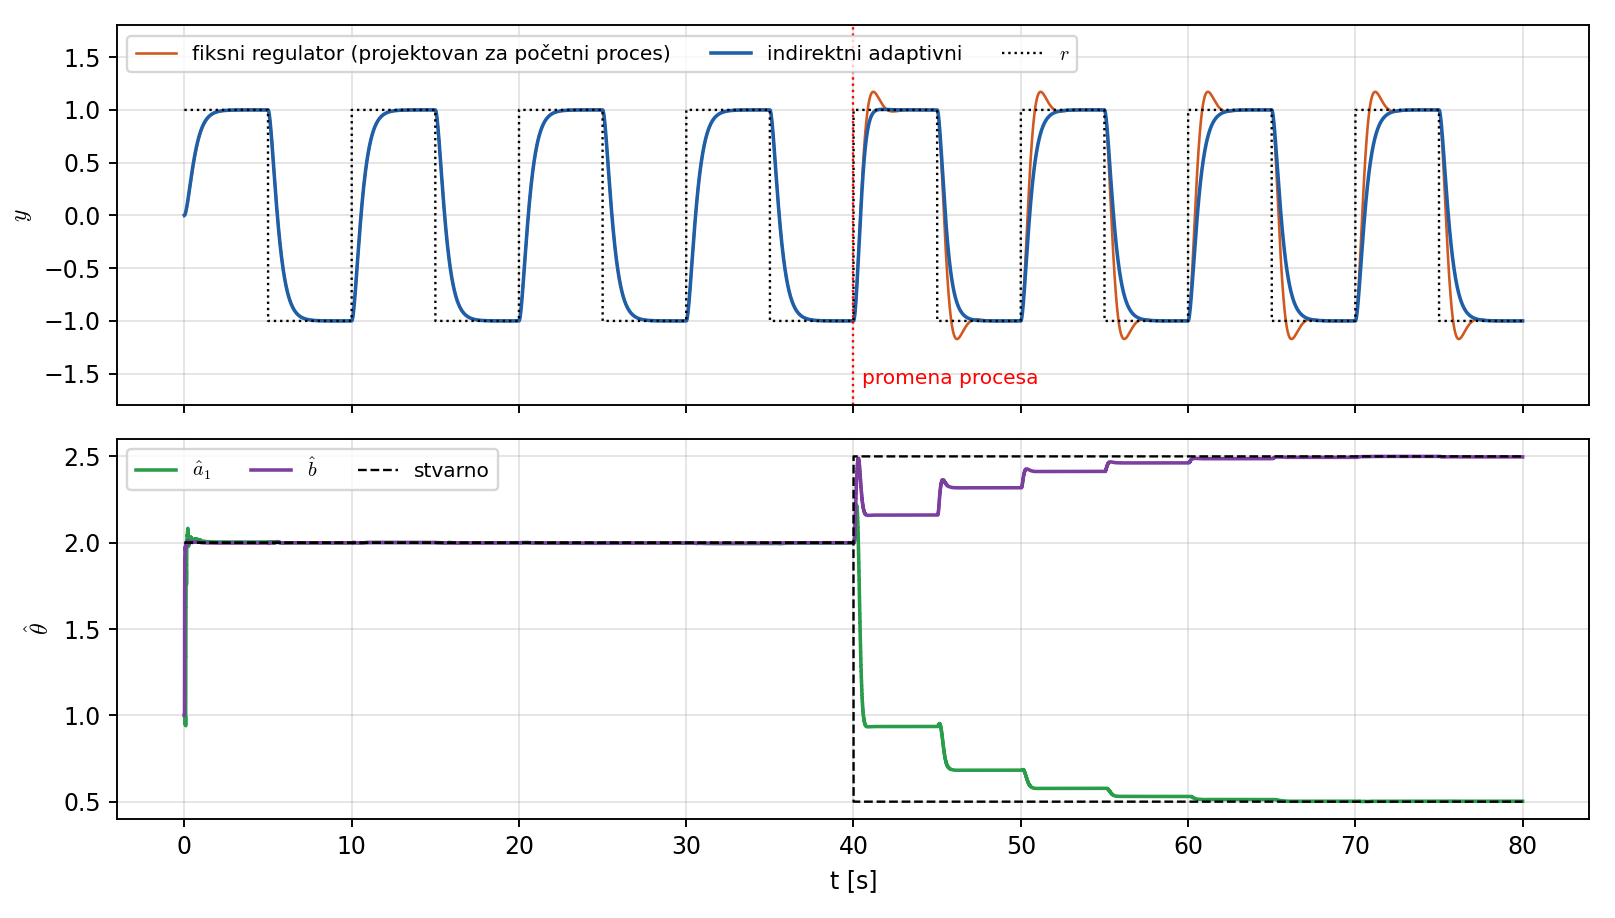
\includegraphics[width=0.95\linewidth,height=\textheight,keepaspectratio,alt={Gore: fiksni regulator (projektovan za početni proces) i indirektni adaptivni. Posle promene procesa fiksni ima preskok (vrh 1,17 pri skoku sa −1 na 1, oko 8 \%), a adaptivni zadržava oblik odziva bez preskoka. Dole: procene â1 i b̂ konvergiraju ka novim vrednostima u stepenicama, na svakom skoku reference}]{figures/projekat_stanja.png}
\caption{Gore: fiksni regulator (projektovan za početni proces) i indirektni adaptivni. Posle promene procesa fiksni ima preskok (vrh 1,17 pri skoku sa −1 na 1, oko 8 \%), a adaptivni zadržava oblik odziva bez preskoka. Dole: procene â1 i b̂ konvergiraju ka novim vrednostima u stepenicama, na svakom skoku reference}
\end{figure}

Šta se vidi i šta treba reći na odbrani:

\begin{itemize}
\item \textbf{Fiksni regulator} ostaje stabilan, ali mu se polovi pomere (dobija se \(-2{,}07 \pm 2{,}66j\) umesto \(-3, -3\)), pa odziv dobije preskok. To je motivacija za adaptivno upravljanje: „polovi koje smo podesili više nisu tamo gde želimo''.
\item \textbf{Adaptivni} vraća polove blizu željenih mesta.
\item Procene se menjaju \textbf{u stepenicama}: samo na skokovima reference ima nove informacije. Između skokova sistem miruje i procena stoji. To je uslov dovoljne pobude uživo. Referenca je istovremeno i pobuda za estimator.
\item Ovo je \textbf{identifikacija u zatvorenoj sprezi}: \(u\) zavisi od \(y\). Radi zato što referenca daje spoljašnju pobudu koja ne zavisi od šuma.
\end{itemize}

\textbf{Kako to sklopiti u Simulinku (varijanta A).}

\begin{enumerate}
\def\labelenumi{\arabic{enumi}.}
\item \emph{Proces:} kontinualni blok (\emph{Transfer Fcn} ili \emph{State-Space}); promena procesa preko \emph{Clock} + \emph{Switch} između dva bloka.
\item \emph{Filtri:} četiri bloka \(\frac{s^m}{(T_fs+1)^2}\) (za \(\ddot y_f\), \(\dot y_f\), \(y_f\), \(u_f\)), kao u poglavlju o MNK. Za \(u\) se uzima isti signal koji ulazi u proces.
\item \emph{RLS:} MATLAB Function sa \emph{Sample time} \(T_s\) (kod iz poglavlja o RLS-u, sa \(\varphi = [-\dot y_f;\ u_f]\)), sa projekcijom \(\hat b \ge b_{min}\) na kraju.
\item \emph{Projektovanje:} MATLAB Function (isti \(T_s\)) koji iz \(\hat\theta\) računa \(K\), \(L\), \(k_r\) po formulama iznad. Formule u zatvorenom obliku su sigurnije od \texttt{acker} u svakom koraku.
\item \emph{Observer stanja i poremećaja:} matrice se menjaju u vremenu, pa ne može blok \emph{State-Space} (on ima fiksne matrice). Umesto toga MATLAB Function računa \(\dot{\hat x}\) i \(\dot{\hat d}\) po jednačinama iznad, a blok \emph{Integrator} (sa 3 stanja) daje \(\hat x\) i \(\hat d\) (referentni skript radi isto za \(\hat x\), Ojlerom). Integrator prekida algebarsku petlju \(\hat x \to u \to \dot{\hat x}\).
\item \emph{Zakon upravljanja:} \(u = -K\hat x - \hat d + k_rr\); referenca iz \emph{Pulse Generator} (\(\pm1\), perioda 10 s); poremećaj \(d\) kao \emph{Step} na ulazu procesa, uključen kasnije u simulaciji.
\item \emph{Prekidač „adaptacija uključena/isključena''} (npr. \emph{Manual Switch} koji zamrzava \(\hat\theta\)): tako se na odbrani lako pokaže fiksni naspram adaptivnog regulatora.
\end{enumerate}

Hijerarhija brzina iz primera: regulator \(3\) \textless{} observer \(12\) \textless{} filter \(1/T_f = 20\) \textless{} odabiranje \(1/T_s = 100\) \textless{} korak solvera \(1/h = 1000\) (sve u rad/s ili 1/s). Svaki sloj treba da bude nekoliko puta brži od prethodnog. Ako menjaš neki broj, proveri da redosled ostane.

\subsection{Varijanta B: diskretni model sa estimatorom poremećaja}

Referentno rešenje projekta (putanja je u mapi domaćih) je potpuno diskretno i ima estimator poremećaja. Njegova struktura, pročitana iz \texttt{projekat.m}, \texttt{update\_\allowbreak{}controller.m}, \texttt{update\_\allowbreak{}estimator.m} i MATLAB Function blokova u \texttt{projekat\_\allowbreak{}model.slx}:

\textbf{Proces i promena.} \(T_s = 1\) ms. Dva kontinualna procesa \(\frac{b_0}{s^2 + a_1s + a_0}\) diskretizovana sa \texttt{c2d}:

\begin{itemize}
\item sistem 1: \(a_0 = 8\), \(a_1 = 7\), \(b_0 = 5\), tj. \(\frac{5}{(s+1)(s+7)}\);
\item sistem 2: \(a_0 = 1\), \(a_1 = 6\), \(b_0 = 3\), tj. \(\frac{3}{s^2 + 6s + 1}\).
\end{itemize}

Switch prebacuje sa sistema 1 na sistem 2 u \(t = 20\) s. Na ulaz procesa dodaje se i odskočni poremećaj.

\textbf{Estimator parametara (RLS).} Diskretna funkcija prenosa drugog reda posle \texttt{c2d} ima oblik \(\frac{b_1z + b_0}{z^2 + a_1z + a_0}\), pa je ARX model

\[y(k) = -a_1y(k-1) - a_0y(k-2) + b_1u(k-1) + b_0u(k-2),\qquad \theta = [a_1\;\; a_0\;\; b_1\;\; b_0]^T .\]

U kodu se ulazi zovu \texttt{ddot\_\allowbreak{}y,\allowbreak{}\ dot\_\allowbreak{}y,\allowbreak{}\ y,\allowbreak{}\ dot\_\allowbreak{}u,\allowbreak{}\ u}, ali po vezama u Simulinku to su \(y_f(k)\), \(y_f(k-1)\), \(y_f(k-2)\), \(u_f(k-1)\), \(u_f(k-2)\) (blokovi \emph{Delay} dužine 1 i 2). Imena su ostala iz kontinualne verzije. Oba signala prolaze kroz isti diskretni filtar \(\frac{1}{\left(\frac{T_f}{T_s}z + 1 - \frac{T_f}{T_s}\right)^2}\) (Ojlerova diskretizacija \(\frac{1}{(T_fs+1)^2}\), \(T_f = 10\) ms, pol u \(z = 0{,}9\)). RLS ima \(\lambda = 0{,}999\) i \(P_0 = 10^9I\), a \(\hat\theta_0 = 0\) (dozvoljeno, jer prva faza radi bez regulatora).

Zašto tako veliko \(P_0\) i tako bogata pobuda? Sa \(T_s = 1\) ms diskretni model procesa \(\frac{5}{(s+1)(s+7)}\) je (\texttt{c2d}, ZOH)

\[G(z) = \frac{2{,}494\cdot10^{-6}z + 2{,}488\cdot10^{-6}}{z^2 - 1{,}99302z + 0{,}99302}.\]

Koeficijenti \(b\) su sitni, a \(a_1\), \(a_0\) su blizu \(-2\) i \(1\), jer se za kratko \(T_s\) signal između dva odbirka skoro ne promeni. Regresor je loše uslovljen, i mala relativna greška u \(\hat a_1\), \(\hat a_0\) pomera polove modela mnogo. Sa \(T_s = 10\) ms bilo bi \(b \approx 2{,}4\cdot10^{-4}\) i \(a_1 \approx -1{,}93\), tj. identifikacija je lakša. Ako praviš svoju diskretnu varijantu, ne biraj \(T_s\) manje nego što traži pravilo \(|p|T_s \approx 0{,}05\) do \(0{,}2\) (pregled na početku).

\textbf{Smenjivanje identifikacije i upravljanja.} Vreme se deli na prozore od 20 s (\texttt{upd\ =\ 20}, \texttt{sw\ =\ 10}):

\begin{itemize}
\item \(\operatorname{mod}(t, 20) \le 10\): \textbf{faza identifikacije}. Proces se pobuđuje u otvorenoj sprezi generatorom \(u = 1 + \sum_{f=1}^{50}\sin(2\pi ft)\), a RLS radi;
\item \(\operatorname{mod}(t, 20) > 10\): \textbf{faza upravljanja}. Regulator je uključen, procena je zamrznuta, a \(P\) se resetuje na \(P_0\), da bi sledeća identifikacija krenula „sveže''.
\end{itemize}

Tako je pobuda uvek bogata, ali proces pola vremena radi bez regulatora. U stvarnom postrojenju to obično nije prihvatljivo. Varijanta A uči istovremeno sa upravljanjem, pa je bliža onome što je rečeno na predavanju („radi u realnom vremenu, \texttt{while(1)}„). Bolje je znati obe i umeti da objasniš razliku.

\textbf{Regulator} (\texttt{update\_\allowbreak{}controller.m}). Model u upravljivoj kanoničnoj formi:

\[A = \begin{bmatrix}0 & 1\\ -\hat a_0 & -\hat a_1\end{bmatrix},\qquad B = \begin{bmatrix}0\\ 1\end{bmatrix},\qquad C = [\hat b_0\;\; \hat b_1],\]

jer je tada \(C(zI - A)^{-1}B = \frac{\hat b_1z + \hat b_0}{z^2 + \hat a_1z + \hat a_0}\). Polovi: \texttt{acker(\allowbreak{}A,\allowbreak{}\ B,\allowbreak{}\ {[}exp(\allowbreak{}-5e-3),\allowbreak{}\ exp(\allowbreak{}-5e-3){]})}, tj. dvostruki pol \(z = e^{-5T_s}\), što odgovara \(s = -5\).

\textbf{\(k_r\) u diskretnom obliku.} \(A - BK = \begin{bmatrix}0 & 1\\ -(\hat a_0 + k_1) & -(\hat a_1 + k_2)\end{bmatrix}\), pa je

\[G_{cl}(z) = \frac{\hat b_1z + \hat b_0}{z^2 + (\hat a_1 + k_2)z + (\hat a_0 + k_1)},\qquad G_{cl}(1) = \frac{\hat b_1 + \hat b_0}{1 + \hat a_1 + \hat a_0 + k_1 + k_2},\]

\[k_r = \frac{1 + \hat a_1 + \hat a_0 + k_1 + k_2}{\hat b_1 + \hat b_0} .\]

Tačno tako piše u bloku „Kontroler'' referentnog rešenja. Upravljanje je \(u = -K\hat x + k_rr\), a na ulaz procesa ide \(u - \hat d\).

\textbf{Observer stanja i poremećaja} (\texttt{update\_\allowbreak{}estimator.m}). Konstantan poremećaj u diskretnom vremenu: \(A_w = 1\), \(C_w = 1\). Prošireni model i pojačanje:

\[\bar A = \begin{bmatrix}A & BC_w\\ 0\;\;0 & A_w\end{bmatrix},\qquad \bar C = [C\;\; 0],\qquad L = \texttt{place}(\bar A', \bar C', p_{est})' .\]

\texttt{place} traži različite polove, zato su izabrani \(e^{-15T_s}\), \(e^{-16T_s}\), \(e^{-17T_s}\) (oko \(s = -15, -16, -17\), tri puta brže od regulatora). Observer je prediktorskog oblika:

\[\hat x(k+1) = (A - L_xC)\hat x(k) + Bu(k) + L_xy(k),\qquad \hat w(k+1) = \hat w(k) + L_w\big(y(k) - C\hat x(k)\big),\qquad \hat d = \hat w .\]

\begin{ispit}
Ako budeš koristio referentno rešenje kao polazište, proveri tri stvari (detalji u spisku otvorenih pitanja): (1) u \texttt{update\_\allowbreak{}estimator.m} prvi pol je \texttt{-exp(\allowbreak{}-15*1e-3)}, sa minusom, tj. \(z \approx -0{,}985\), što je gotovo sigurno greška u kucanju; (2) u bloku „Estimator stanja'' nedostaje član \(B\hat w\), koji prošireni model \(\bar A\) podrazumeva; (3) observer dobija \(u\) \textbf{pre} oduzimanja \(\hat d\). Dosledno je: u observer ide stvarno primenjeno \(u - \hat d\), a jednačina stanja ima \(B(u_{prim} + \hat w)\).
\end{ispit}

\textbf{Poremećaj kvari RLS.} Sa konstantnim \(d\) na ulazu procesa ARX jednačina postaje

\[y(k) = -a_1y(k-1) - a_0y(k-2) + b_1u(k-1) + b_0u(k-2) + (b_1 + b_0)\,d .\]

Poslednji član nije u \(\varphi\), pa ga RLS „objasni'' pogrešnim \(\hat\theta\) (pristrasna procena). Isto važi i za filtrirane signale, jer filter \(\frac{1}{(T_fs+1)^2}\) propušta konstantu. Primer sa predavanja \izvor{P09 snimak, 62.--67. min}: proces je samo pojačanje 3, ulaz 1, a na ulazu je konstantan poremećaj 2; izlaz je \(3(1 + 2) = 9\), pa estimator koji ne zna za \(d\) proceni pojačanje 9 umesto 3.

\textbf{Glavni lek (sa predavanja): propusnik opsega} \izvor{P09 snimak, 77.--87. min}. Signale za identifikaciju (\(u\) i \(y\), isti filter na oba) ne provlačiti samo kroz niskopropusni filter, nego kroz \textbf{propusnik opsega}, npr.

\[F(s) = \frac{T_1s}{(T_1s+1)(T_2s+1)},\qquad T_1 > T_2 .\]

Visokopropusni deo (nula u \(s = 0\)) uklanja konstantu od \(d\), a niskopropusni deo guši šum; u opsegu od \(1/T_1\) do \(1/T_2\) pojačanje je približno 1. Pošto je filter isti za \(u\) i \(y\), odnos \(u \to y\) (dakle \(\theta\)) se ne menja, kao kod filtara u poglavlju o MNK. Pobuda (skokovi reference, dither) mora da pada u propusni opseg. Za kontinualni model sa filtrima \(\frac{s^m}{(T_fs+1)^2}\) dovoljno je svim filtrima dodati isti visokopropusni faktor \(\frac{T_1s}{T_1s+1}\); kolone sa \(m \ge 1\) ionako ne propuštaju konstantu, problem su \(y_f\) i \(u_f\). Posle toga su procene tačne, a sam poremećaj kompenzuje estimator poremećaja u observeru, „i tu je zatvorena cela priča''. (Na predavanju je opseg zadat kao „1--10 Hz'' sa \(T_1 = 1\), \(T_2 = 0{,}1\); te vremenske konstante zapravo daju opseg 1--10 rad/s.)

Alternative:

\begin{enumerate}
\def\labelenumi{\arabic{enumi}.}
\item proširiti \(\varphi\) jedinicom, \(\varphi = [\dots;\ 1]\), pa je poslednji parametar \(\theta_d = (b_1 + b_0)d\) (na predavanju za pojačanje \(b_0\): \(\theta_d = b_0c\), pa je \(\hat c = \hat\theta_d/\hat b_0\)). Tada ne treba observer poremećaja, ali „možda nije najsrećnije'': ako se identifikator isključi (fiksni režim), nema ni integratora ni estimatora poremećaja i ništa ne radi kako treba \izvor{P09 snimak, 68.--78. min};
\item raditi sa razlikama \(\Delta y(k) = y(k) - y(k-1)\) i \(\Delta u(k)\), koje zadovoljavaju istu jednačinu bez \(d\) (razlika je najprostiji diskretni visokopropusni filter, dakle isti princip kao propusnik opsega);
\item identifikovati samo kad poremećaja nema, npr. na početku, pre uključenja regulacije.
\end{enumerate}

Ako se poremećaj u simulaciji uključuje dok RLS radi, pogledaj da li \(\hat\theta\) u tom trenutku skače.

\textbf{Start adaptacije i režimi rada} \izvor{P09 snimak, 75.--78. i 98.--101. min}. Tri načina da estimator na početku dobije dobru pobudu i procenu: (1) ako je proces stabilan, prvo kratka identifikacija u otvorenoj sprezi, pa uključenje regulacije; (2) na konstantnu referencu dodati zbir malih sinusoida koje nisu prebrze (da ih filter ne poništi); (3) početi sa regulatorom sa nominalnim (fiksnim) parametrima, pa preći na adaptivni kad se \(\hat\theta\) ustali. Adaptivni regulator u praksi ima tri režima: ručni, sa fiksnim parametrima (identifikator isključen) i pun adaptivni.

\subsection{Varijanta sa RST regulatorom}

Umesto \(K\), \(L\), \(k_r\) može se u svakom koraku rešiti Diofantova jednačina \(\hat A R + \hat B S = A_{cl}^*\) i izračunati \(T = A_{cl}^*(0)/\hat B(0)\) (poglavlje o RST regulatoru). Integrator u \(R\) tada sam potiskuje konstantni poremećaj, bez posebnog estimatora. Na predavanju je za projekat pominjan regulator po stanjima sa observerom, pa je RST varijanta opcija, ne zahtev.

\subsection{Izbor parametara: kratka lista}

\begin{longtable}[]{@{}
  >{\raggedright\arraybackslash}p{(\linewidth - 4\tabcolsep) * \real{0.2632}}
  >{\raggedright\arraybackslash}p{(\linewidth - 4\tabcolsep) * \real{0.3684}}
  >{\raggedright\arraybackslash}p{(\linewidth - 4\tabcolsep) * \real{0.3684}}@{}}
\caption{Preporučene vrednosti za projekat}\tabularnewline
\toprule\noalign{}
\begin{minipage}[b]{\linewidth}\raggedright
Parametar
\end{minipage} & \begin{minipage}[b]{\linewidth}\raggedright
Preporuka
\end{minipage} & \begin{minipage}[b]{\linewidth}\raggedright
Zašto
\end{minipage} \\
\midrule\noalign{}
\endfirsthead
\toprule\noalign{}
\begin{minipage}[b]{\linewidth}\raggedright
Parametar
\end{minipage} & \begin{minipage}[b]{\linewidth}\raggedright
Preporuka
\end{minipage} & \begin{minipage}[b]{\linewidth}\raggedright
Zašto
\end{minipage} \\
\midrule\noalign{}
\endhead
\bottomrule\noalign{}
\endlastfoot
broj parametara u \(\theta\) & samo nepoznati; poznatu strukturu (integrator) ne procenjivati & manje nepoznatih, manje pobude \\
\(\lambda\) & 0,99 do 0,999; memorija \(T_s/(1-\lambda)\) oko nekoliko sekundi & brzina praćenja naspram šuma \\
\(P_0\) & \(\alpha I\), \(\alpha \gg 1\) (predavanje); \(10^2\) do \(10^4\) za signale reda 1, loše uslovljen diskretni ARX traži više (referentni projekat \(10^9\)) & brz početak; \(\alpha\lVert\varphi\rVert^2 \gg 1\) je standardna praksa, nije rečeno na predavanju \\
\(\hat\theta_0\) & nominalni model, ne nula (osim ako regulator na početku ne radi) & \(\hat b = 0\) daje neupravljiv model \\
\(T_f\) & \(1/T_f\) brže od polova observera, a \(T_f\) nekoliko puta veće od \(T_s\) & izvodi bez previše šuma, filter ne kasni za petljom \\
\(T_s\) & na predavanju oko 0,1 s za sisteme sa kursa; \(\lvert p\rvert T_s \approx 0{,}05\) do \(0{,}2\) za najbrži pol petlje (standardna praksa, nije rečeno na predavanju) & dovoljno odbiraka, a diskretni model ne postane loše uslovljen \\
polovi regulatora & istog reda kao polovi procesa, do oko 3 puta brži (standardna praksa, nije rečeno na predavanju) & veliki \(K\) znači veliko \(u\) i osetljivost na grešku modela \\
polovi observera (i poremećaja) & bar 4 puta brži od regulatora (potvrđeno na predavanju) & separacija, regulator radi sa dobrom procenom \\
referenca & pravougaona, ili dodati mali dither (potvrđeno na predavanju) & pobuda za estimator \\
projekcija & \(\hat b \ge b_{min} > 0\) & model mora ostati upravljiv \\
filter za identifikaciju & propusnik opsega, isti za \(u\) i \(y\) (sa predavanja) & konstantni \(d\) ne kvari procenu \\
\end{longtable}

\subsection{Šta pokazati na odbrani}

\begin{enumerate}
\def\labelenumi{\arabic{enumi}.}
\item Šemu i ulogu svakog bloka (tabela gore).
\item Grafik \(\hat\theta(t)\) sa stvarnim vrednostima: konvergencija na početku i posle promene procesa.
\item Grafik \(y\), \(r\) (i \(u\)): fiksni regulator naspram adaptivnog posle promene procesa.
\item Uticaj \(\lambda\) ili \(\Gamma\) na brzinu praćenja i na šum (dve simulacije).
\item Šta se desi bez pobude (konstantna referenca): procena stoji, \(P\) raste.
\item Estimator poremećaja (deo zadatka po P09): \(d\) i \(\hat d\), i izlaz bez trajne greške; uz to \(\hat\theta\) sa i bez propusnika opsega posle uključenja \(d\).
\item Prekidač adaptacije: isti poremećaj ili promena procesa sa zamrznutim i sa aktivnim \(\hat\theta\).
\end{enumerate}

Kako izgleda „radi'':

\begin{itemize}
\item \(\hat\theta\) stigne na tačne vrednosti (na nekoliko procenata) posle nekoliko perioda reference, i posle promene procesa ponovo za vreme reda memorije \(T_s/(1-\lambda)\);
\item posle konvergencije \(y\) ima oblik koji daju zadati polovi (za dvostruki pol u \(-3\): bez preskoka, smirenje za oko \(5{,}8/3 \approx 2\) s), i pre i posle promene procesa; fiksni regulator posle promene odstupa;
\item \(\hat y = C\hat x\) prati \(y\) (kod varijante B stanja nisu fizička, pa se porede samo izlazi);
\item kontrola na kraju simulacije: sopstvene vrednosti cele petlje sa \textbf{stvarnim} procesom i poslednjim \(K\), \(L\) treba da budu blizu zadatih polova regulatora i observera. Referentni skript to računa sa \texttt{eig} nad matricom \(\begin{bmatrix}A & -BK\\ LC & \hat A - \hat BK - LC\end{bmatrix}\) (stanja \(x\) i \(\hat x\));
\item \(u\) nema ogromne skokove pri promeni procesa. Ako ima, \(\hat b\) je verovatno prošlo blizu nule (proveri projekciju).
\end{itemize}

\begin{ispit}
Tipična pitanja: zašto „indirektno'' (procenjuju se parametri procesa, pa se regulator računa iz njih), šta je certainty equivalence, zašto se \(k_r\) preračunava zajedno sa \(K\), zašto je observer brži, zašto je referenca pravougaona, šta se desi kad \(\hat b \to 0\), kako \(\lambda\) utiče na odziv posle promene procesa, da li estimator radi u otvorenoj ili zatvorenoj sprezi, zašto poremećaj pokvari procenu i kako to rešava propusnik opsega, i zašto se \(\hat d\) procenjuje u observeru, a ne jedinicom u \(\varphi\) (radi i kad je identifikator isključen).
\end{ispit}

\section{Mapa domaćih zadataka i projekta}

\subsection{Kako čitati ovu mapu}

Zvaničan tekst domaćih kod prof. Rapajića nije među materijalima. Tekstovi ispod su \textbf{diktirani na predavanjima}: P01--P06 i audio snimci drži prof. Mirna Radović, a P07--P09 predavačica iz njenog tima (verovatno asistentkinja). To je dakle verzija zadataka prof. Radović; ako prof. Rapajić zada drugačije, važe njegovi tekstovi. Tabela je rekonstruisana iz tih tekstova i iz foldera sa rešenjima: tvojih (\texttt{Domaci/\allowbreak{}Domaci1–6}) i dva referentna skupa: \textbf{ref. 1} (\texttt{NenadDomaci/\allowbreak{}.../\allowbreak{}Napredno\ upravljanje/\allowbreak{}Domaci/\allowbreak{}domaci1–6}, novija generacija) i \textbf{ref. 2} (\texttt{AnjaMaterijali/\allowbreak{}domaci/\allowbreak{}matlab/\allowbreak{}adaptivno}, generacija kod prof. Radović, drugačija numeracija). Kolona „Poglavlje'' pokazuje gde je teorija u ovim beleškama.

\begin{longtable}[]{@{}
  >{\raggedright\arraybackslash}p{(\linewidth - 10\tabcolsep) * \real{0.1420}}
  >{\raggedright\arraybackslash}p{(\linewidth - 10\tabcolsep) * \real{0.3479}}
  >{\raggedright\arraybackslash}p{(\linewidth - 10\tabcolsep) * \real{0.1775}}
  >{\raggedright\arraybackslash}p{(\linewidth - 10\tabcolsep) * \real{0.1207}}
  >{\raggedright\arraybackslash}p{(\linewidth - 10\tabcolsep) * \real{0.1110}}
  >{\raggedright\arraybackslash}p{(\linewidth - 10\tabcolsep) * \real{0.1009}}@{}}
\caption{Domaći zadaci, teorija i postojeća rešenja}\tabularnewline
\toprule\noalign{}
\begin{minipage}[b]{\linewidth}\raggedright
Tvoj domaći
\end{minipage} & \begin{minipage}[b]{\linewidth}\raggedright
Tema
\end{minipage} & \begin{minipage}[b]{\linewidth}\raggedright
Poglavlje
\end{minipage} & \begin{minipage}[b]{\linewidth}\raggedright
Tvoje rešenje
\end{minipage} & \begin{minipage}[b]{\linewidth}\raggedright
Ref. 1
\end{minipage} & \begin{minipage}[b]{\linewidth}\raggedright
Ref. 2
\end{minipage} \\
\midrule\noalign{}
\endfirsthead
\toprule\noalign{}
\begin{minipage}[b]{\linewidth}\raggedright
Tvoj domaći
\end{minipage} & \begin{minipage}[b]{\linewidth}\raggedright
Tema
\end{minipage} & \begin{minipage}[b]{\linewidth}\raggedright
Poglavlje
\end{minipage} & \begin{minipage}[b]{\linewidth}\raggedright
Tvoje rešenje
\end{minipage} & \begin{minipage}[b]{\linewidth}\raggedright
Ref. 1
\end{minipage} & \begin{minipage}[b]{\linewidth}\raggedright
Ref. 2
\end{minipage} \\
\midrule\noalign{}
\endhead
\bottomrule\noalign{}
\endlastfoot
1 & statički/dinamički, linearnost, Bode & Modelovanje & \texttt{Domaci1/\allowbreak{}zad1..3} & \texttt{domaci1} & \texttt{zad1} \\
2 & identifikacija, MNK (kontinualno i diskretno) & MNK & \texttt{Domaci2} & \texttt{domaci6/\allowbreak{}domaci6\_\allowbreak{}1.m} & \texttt{zad2} \\
3 & regulator po stanjima, \(k_r\) & Regulator po stanjima & \texttt{Domaci3} & \texttt{domaci2} & --- \\
4 & observer, regulator po izlazima & Observer & \texttt{Domaci4} & \texttt{domaci3} & --- \\
5 & estimator poremećaja & Poremećaji & \texttt{Domaci5} & \texttt{domaci4} & --- \\
6 & RST, potiskivanje poremećaja & RST & \texttt{Domaci6} & \texttt{domaci5} & \texttt{zad3a–c} \\
zadat na P08/P09 & RLS, faktor zaboravljanja, propusnik opsega & RLS & --- & \texttt{domaci6/\allowbreak{}domaci6\_\allowbreak{}2.m} & \texttt{zad4} \\
zadat na P08 & gradijentni algoritam & Gradijent & --- & \texttt{domaci6/\allowbreak{}domaci6\_\allowbreak{}3.m} & \texttt{zad5} \\
projekat & indirektno adaptivno upravljanje & Projekat & --- & \texttt{projekat/} & \texttt{zad6} \\
\end{longtable}

Na predavanju P07 je RST domaći nazvan „domaći 5'' (tvoja numeracija ima ga kao 6); RLS i gradijent su takođe zadati kao domaći (tekstovi ispod).

Ref. 2 ima i beleške „šta reći na odbrani'' (\texttt{AnjaMaterijali/\allowbreak{}domaci/\allowbreak{}beleske\ -\ adaptivno/\allowbreak{}Beleske\ 1–6}), a zbirni opis sa rezultatima je u \texttt{DZ\ -\ Adaptivno\ upravljanje.md}.

\subsection{Tekstovi zadataka sa predavanja}

\textbf{D1 (modelovanje) → poglavlje Modelovanje} \izvor{P01 snimak, 83.--90. min}.

\begin{enumerate}
\def\labelenumi{\arabic{enumi}.}
\item Uzeti jedan statički (npr. \(y = 4u + 3\)) i jedan dinamički sistem (npr. \(\frac{1}{s^2+s+1}\), „koji god hoćete''), simulirati proizvoljan ulaz (beli šum, slučajan signal), pa \textbf{zaboraviti model} i samo iz snimljenih \(u\), \(y\) odrediti da li je sistem statički ili dinamički.
\item Za jedan linearan i jedan nelinearan sistem (npr. sa proizvodom ili kvadratom signala) proveriti linearnost preko novih harmonika. Preporuka: ulaz kao zbir sinusoida poznatih učestanosti, da se zna šta treba videti u FFT-u.
\item Za izmišljeni linearan sistem proceniti funkciju prenosa iz Bodeovog dijagrama.
\end{enumerate}

Može i u paru: jedan generiše podatke, drugi „provaljuje'' sistem.

\textbf{D2 (MNK) → poglavlje MNK} \izvor{P02 snimak, 67.--81. i 104.--106. min}. Proces \textbf{drugog reda sa 4 parametra}, \(G(s) = \frac{b_1s + b_0}{s^2 + a_1s + a_0}\) (brojeve izabrati sam):

\begin{enumerate}
\def\labelenumi{\arabic{enumi}.}
\item zapisati \(\eta = \ddot y\), \(\varphi = [-\dot y\;\; -y\;\; \dot u\;\; u]^T\), \(\theta = [a_1\;\; a_0\;\; b_1\;\; b_0]^T\);
\item na ulaz dovesti zbir \textbf{bar 4 sinusoide} različitih učestanosti;
\item \(u\) i \(y\) provući kroz iste filtre \(\frac{s^m}{(T_fs+1)^2}\), \(m = 0, 1, 2\), tako da filter ne odseče ulazne učestanosti;
\item \(\theta\) izračunati pseudoinverzijom (\texttt{pinv} ili \texttt{Phi\textbackslash{}eta}), \textbf{bez i sa mernim šumom}, uz menjanje \(T_f\);
\item isto uraditi za \textbf{diskretni} sistem (pomereni odbirci umesto izvoda, opcioni filter \(\frac{1-\alpha}{z-\alpha}\)).
\end{enumerate}

\textbf{D3/D4 (servo motor) → poglavlje Regulator po stanjima i observer} \izvor{P03 snimak, 122.--124. min; P04 snimak, 20.--30. min}. Na motoru \(\frac{K}{s(Ts+1)}\) sa sopstvenim \(K\) i \(T\): (1) P regulator; (2) PD regulator, npr. \textbf{PD sa filtrom}; (3) regulator po stanjima; (4) estimator stanja; zatim regulator po izlazima. Tvoj motor \(A = \begin{bmatrix}0 & 1\\ 0 & -2\end{bmatrix}\), \(B = \begin{bmatrix}0\\ 4\end{bmatrix}\) odgovara \(K = 2\), \(T = 0{,}5\). Tekst domaćeg za estimator poremećaja nije snimljen (P06 je posle 23. min nečujan).

\textbf{RST → poglavlje RST} {[}P07 snimak, 83.--87. min; snimak Mirna pred snimak1\_2, 15.--17. min{]}. Za „vaš'' motor \(\frac{K}{s(Ts+1)}\) napraviti RST sa potiskivanjem \textbf{konstantnog + sinusnog} poremećaja (i odvojeno i kao zbir), parametre rešiti u MATLAB-u, proveriti simulacijom; zatim isto za \textbf{diskretni} sistem (proces sa \texttt{c2d}, ZOH). Opciono („ko želi bolje''): \textbf{periodični} poremećaj u diskretnom slučaju (\(z^N - 1\) u \(R\)).

\textbf{RLS sa \(\lambda\) → poglavlje RLS} {[}P08 snimak, 111.--129. min; P09 snimak, 34.--35. i 97.--99. min{]}. RLS kao MATLAB Function (\texttt{persistent} \(\hat\theta\) i \(P\)) za proces drugog reda iz D2, pa: (1) dodati \(\lambda\) i uslovno ažuriranje (\textbf{preskakanje ažuriranja} kad je \(\varphi^TP\varphi\) ispod praga); (2) promena parametra procesa u toku simulacije, poređenje \(\lambda = 1\) i \(\lambda < 1\); (3) dodati konstantan \textbf{poremećaj} i pokazati pogrešnu procenu; (4) signale za identifikaciju filtrirati \textbf{propusnikom opsega} i pokazati da je procena ponovo tačna.

\textbf{Gradijent → poglavlje Ljapunov i gradijent} \izvor{P08 snimak, 59.--62. min}. U Simulinku, kontinualno (sa integratorima): (1) proceniti \(\theta\) za \(y = 3u\) (jedan parametar); (2) proceniti parametre procesa \textbf{prvog reda} (dva parametra). U ranijoj generaciji: običan naspram integralnog gradijenta na primeru sa dva parametra.

\textbf{Projekat → poglavlje Projekat} \izvor{P09 snimak, 87.--101. min}. Sve iz prethodnih domaćih u jednoj šemi: procena parametara → \(\hat A\), \(\hat B\), \(\hat C\) → dva \texttt{acker} → observer stanja i poremećaja → \(u = -K\hat x - \hat d + k_rr\). Minimum Simulink, „top'' jedna diskretna MATLAB funkcija (\(r\), \(y\) → \(u\)); sklapati korak po korak.

\subsection{Po zadacima: šta tražiti i na šta paziti}

\textbf{Domaći 1 (modelovanje).} Ref. 1: statički sistem \(3u + 7\), isti sa kašnjenjem, dinamički \(\dot x = -3x + 2u\) (petlja \(y(u)\)) i harmonici. Tvoje: \texttt{zad1\_\allowbreak{}staticki\_\allowbreak{}dinamicki.m} (odskočni test), \texttt{zad2\_\allowbreak{}linearan\_\allowbreak{}nelinearan.m} (superpozicija i FFT), \texttt{zad3\_\allowbreak{}identifikacija\_\allowbreak{}strukture.m} (Bode iz zbira sinusa). Proveri: u \texttt{zad3} je teorijska kriva nacrtana sa \texttt{20*log(\allowbreak{}ampl)}, a treba \texttt{20*log10}; u \texttt{linearan\_\allowbreak{}sistem\_\allowbreak{}bode.m} je simuliran \(\ddot x = -2x + 3u\) (bez prigušenja), a upoređuje se sa \(\frac{1}{s^3 + 6s^2 + 11s + 6}\). Uskladi sistem koji simuliraš i onaj sa kojim porediš. Takođe, u \texttt{zad3} je \(T_s = 0{,}1\) s (Nikvistova učestanost 5 Hz), a \texttt{sin\_\allowbreak{}generator(\allowbreak{}1000,\allowbreak{}\ 0.1,\allowbreak{}\ t)} pravi sinusoide od 0,1 do 100 Hz: sve iznad 5 Hz se preslika (aliasing). Učestanosti su i logaritamski raspoređene, pa ne padaju na mrežu \(k/T_w\) FFT-a (leakage). Uzmi manje \(T_s\) ili samo učestanosti ispod \(1/(5T_s)\), i to celobrojne umnoške \(1/T_w\) (poglavlje o modelovanju).

\textbf{Domaći 2 (MNK).} Tvoje: \texttt{kontinualan\_\allowbreak{}sistem.m} (\(1/(s+2)\) sa filtrima prvog reda) i \texttt{diskretan\_\allowbreak{}sistem.m} (\(y(k) = bu(k) + ay(k-1)\)). To je pojednostavljenje: zadatak sa predavanja je \textbf{drugi red sa 4 parametra}, bez i sa šumom (tekst gore), i njemu odgovara ref. 1. U kontinualnom proveri znak \texttt{b\_\allowbreak{}hat\ =\ -Theta(\allowbreak{}1)} (poglavlje o MNK). Ref. 1 \texttt{domaci6\_\allowbreak{}1.m} radi \(\frac{s+4}{s^2+5s+6}\) sa četiri parametra i diskretni \(\frac{z - 0{,}2}{z^2 - 0{,}4z + 0{,}03}\). Ref. 2 \texttt{zad2} pokazuje rang pri konstantnom ulazu i pristrasnost.

\textbf{Domaći 3 i 4 (stanja, observer).} Tvoje i sa vežbi: motor \(A = \begin{bmatrix}0 & 1\\ 0 & -2\end{bmatrix}\), \(B = \begin{bmatrix}0\\ 4\end{bmatrix}\), \texttt{acker}, \texttt{kr\ =\ 1/\allowbreak{}dcgain(\allowbreak{}...)}, observer kao \emph{State-Space} blok (\(A_o\), \(B_o\), \(C_o = I\)). Tvoj \texttt{Domaci3/\allowbreak{}reg\_\allowbreak{}po\_\allowbreak{}stanjima.m} koristi \(A = \begin{bmatrix}0 & -1\\ 1 & 1\end{bmatrix}\) iz primera sa predavanja. Ref. 1 \texttt{domaci2} proverava i \texttt{rank(\allowbreak{}ctrb(\allowbreak{}A,\allowbreak{}B))}.

\textbf{Domaći 5 (poremećaj).} Proveri \(AA\) i \(CC\) (poglavlje o poremećajima): za poremećaj na ulazu \(AA = \begin{bmatrix}A & BC_w\\ 0 & A_w\end{bmatrix}\), \(CC = [C\;\; 0]\). Tvoj \texttt{estimator\_\allowbreak{}poremecaja\_\allowbreak{}kombinovano.m} ima \(AA = \begin{bmatrix}A & 0\\ 0 & A_w\end{bmatrix}\) i \(CC = [C\;\; C_w]\) (model izlaznog poremećaja), a u \texttt{Vezbe3} je \(CC = [1\;\; 0]\), pa dimenzija ne odgovara matrici \(3\times 3\) (treba \([1\;\; 0\;\; 0]\)). Ref. 1 \texttt{domaci4.m} je dosledan i može da posluži za poređenje. U \texttt{estimator\_\allowbreak{}poremecaja.m} je \texttt{kr\ =\ d/\allowbreak{}dcgain(\allowbreak{}G)}; \(k_r\) ne zavisi od \(d\), pa treba \texttt{1/\allowbreak{}dcgain(\allowbreak{}G)} (radi samo zato što je \(d = 1\)).

\textbf{Domaći 6 (RST).} Tvoj \texttt{rst.m} rešava \(AR + BS = (s+10)^n\) simbolički. Proveri: (1) na početku je \texttt{A\ =\ s*(\allowbreak{}s-1)}, a zadatak sa predavanja je \(\frac{1}{s(s+1)}\); ručno zapisan \(f_{cl}\) u delu sa sinusom odgovara \(s(s+1)\), pa dva dela skripte ne koriste isti proces; (2) \texttt{R\ =\ (\allowbreak{}s\^{}2+w\^{}2)/\allowbreak{}w*(\allowbreak{}s+sigma)} deli sa \(\omega\), pa \(R\) više nije moni, a ručni \(f_{cl}\) pretpostavlja da jeste. Ref. 1 \texttt{domaci5} ima kontinualni i diskretni slučaj (konstanta i sinus) i napomenu kako da se \(G_{ff}\) i \(G_{fb}\) implementiraju kad \(R\) ima korene na jediničnom krugu.

\textbf{RLS i gradijent.} Na predavanjima su zadati kao domaći (tekstovi gore), a potrebni su i za projekat. Ref. 1 \texttt{model6\_2} ima RLS (\(\lambda = 0{,}999\), \(P_0 = 10^4I\), 4 parametra), a \texttt{model6\_3} običan gradijent sa \(\Gamma = 0{,}1I\), \(I\), \(15I\) (poređenje brzine). Ref. 2 \texttt{zad4} i \texttt{zad5} imaju poređenje \(\lambda\) i poređenje običnog i integralnog gradijenta sa šumom.

\textbf{Projekat.} Dve gotove varijante za poređenje: ref. 2 \texttt{zad6} (kontinualno, RLS, motor, bez poremećaja; po P09 mu nedostaje estimator poremećaja) i ref. 1 \texttt{projekat/} (diskretno, smenjivanje identifikacije i upravljanja, estimator poremećaja). Obe su opisane u poglavlju o projektu, zajedno sa mestima koja treba proveriti.

\begin{ispit}
Referentna rešenja služe za proveru, ne za predaju. Na odbrani se pita \textbf{zašto} je nešto urađeno: odakle \(\eta\) i \(\varphi\), zašto baš ti polovi, zašto je observer brži, šta znači \(\lambda\). Za svaki domaći pripremi po jednu rečenicu za svaku jednačinu iz skripte i po jedan grafik koji pokazuje da metoda radi.
\end{ispit}

\end{document}
